\chapter{Angry Real Analysis that will be eventually omitted}



\section[Baby Rudin]{Baby Rudin Independent Study... I need an A and More}
This is the crux of what is meant to be taught and gained. 

\section{Chapter 1 Baby Rudin}


\newpage

\subsection{Pset 1}


\subsubsection*{Problem 1:} \\ 
If r is rational $(r \neq 0)$ and x is irrational, prove that r+x and rx are irrational. \\ 




This is a proof by contradition: \\


Proof: 
\\
Suppose r is rational and $r=\frac{m}{n}$ where m and n are in the set of integers.   \\
Case 1: 
Assume r+x is rational. \\ 
Let r+ x = $\frac{p}{q}$ where p and q are in the set of relatively prime integers.\\ 
Then $x= \frac{p}{q}-r.$ \\ 
$x=\frac{p}{q}-\frac{m}{n}.$ \\ 
$x= \frac{pn-qm}{qn}.$ \\ 
Thus, x is rational, hence a contradiction. \\
Therefore, r+ x is irrational.  \\ 

Case 2: 
Next, assume rx is rational. 
Then $rx =\frac{p}{q}$ where p and q are in the set of integers. \\ 
Then, $x=\frac{p}{rq}.$ \\ 
So, $x= \frac{p}{\frac{m}{n}q}.$ \\ 
$x=\frac{np}{mq}.$ \\ 
Thus, x is rational, hence a contradiction. 
\\ Therefore, rx is irrational. \\ 


\\
Thus, if r is rational and x is irrational, then r+x and rx are irrational. 

\begin{figure}[h]\begin{center}\includegraphics[angle=, origin=c,width=5 in]{Figures/IMG_1052.JPG}
\caption{Placeholder for my proofs} \label{fig:Euler_pic}\end{center}\end{figure} 


\newpage
\subsubsection*{Problem 2:} \\ 
Prove that there is no rational number whose square is 12. \\ 
Proof by contradiction:\\ 
Since $\sqrt{12}=\sqrt{4} \sqrt{3}= 2 \sqrt{3}$,  and from above then $\sqrt{3}$ is irrational. \\ 
Assume that if m and n are integers and have no common factors. \\ 
Since $m^2$ is divisible by 3, then m is divisible by 3. \\  
So $m^2 = 3n^2.$ \\  Let m =3k. \\ 
Then $m^2= 9k^2,$ and we have $3k^2= n^2.$ \\ 
Therefore n is divisible by 3. \\ 
So m and n have no common factor and n is divisible by 3, hence a contradiction.  
\\
Thus, there is no rational number whose square is 12.

\begin{figure}[h]\begin{center}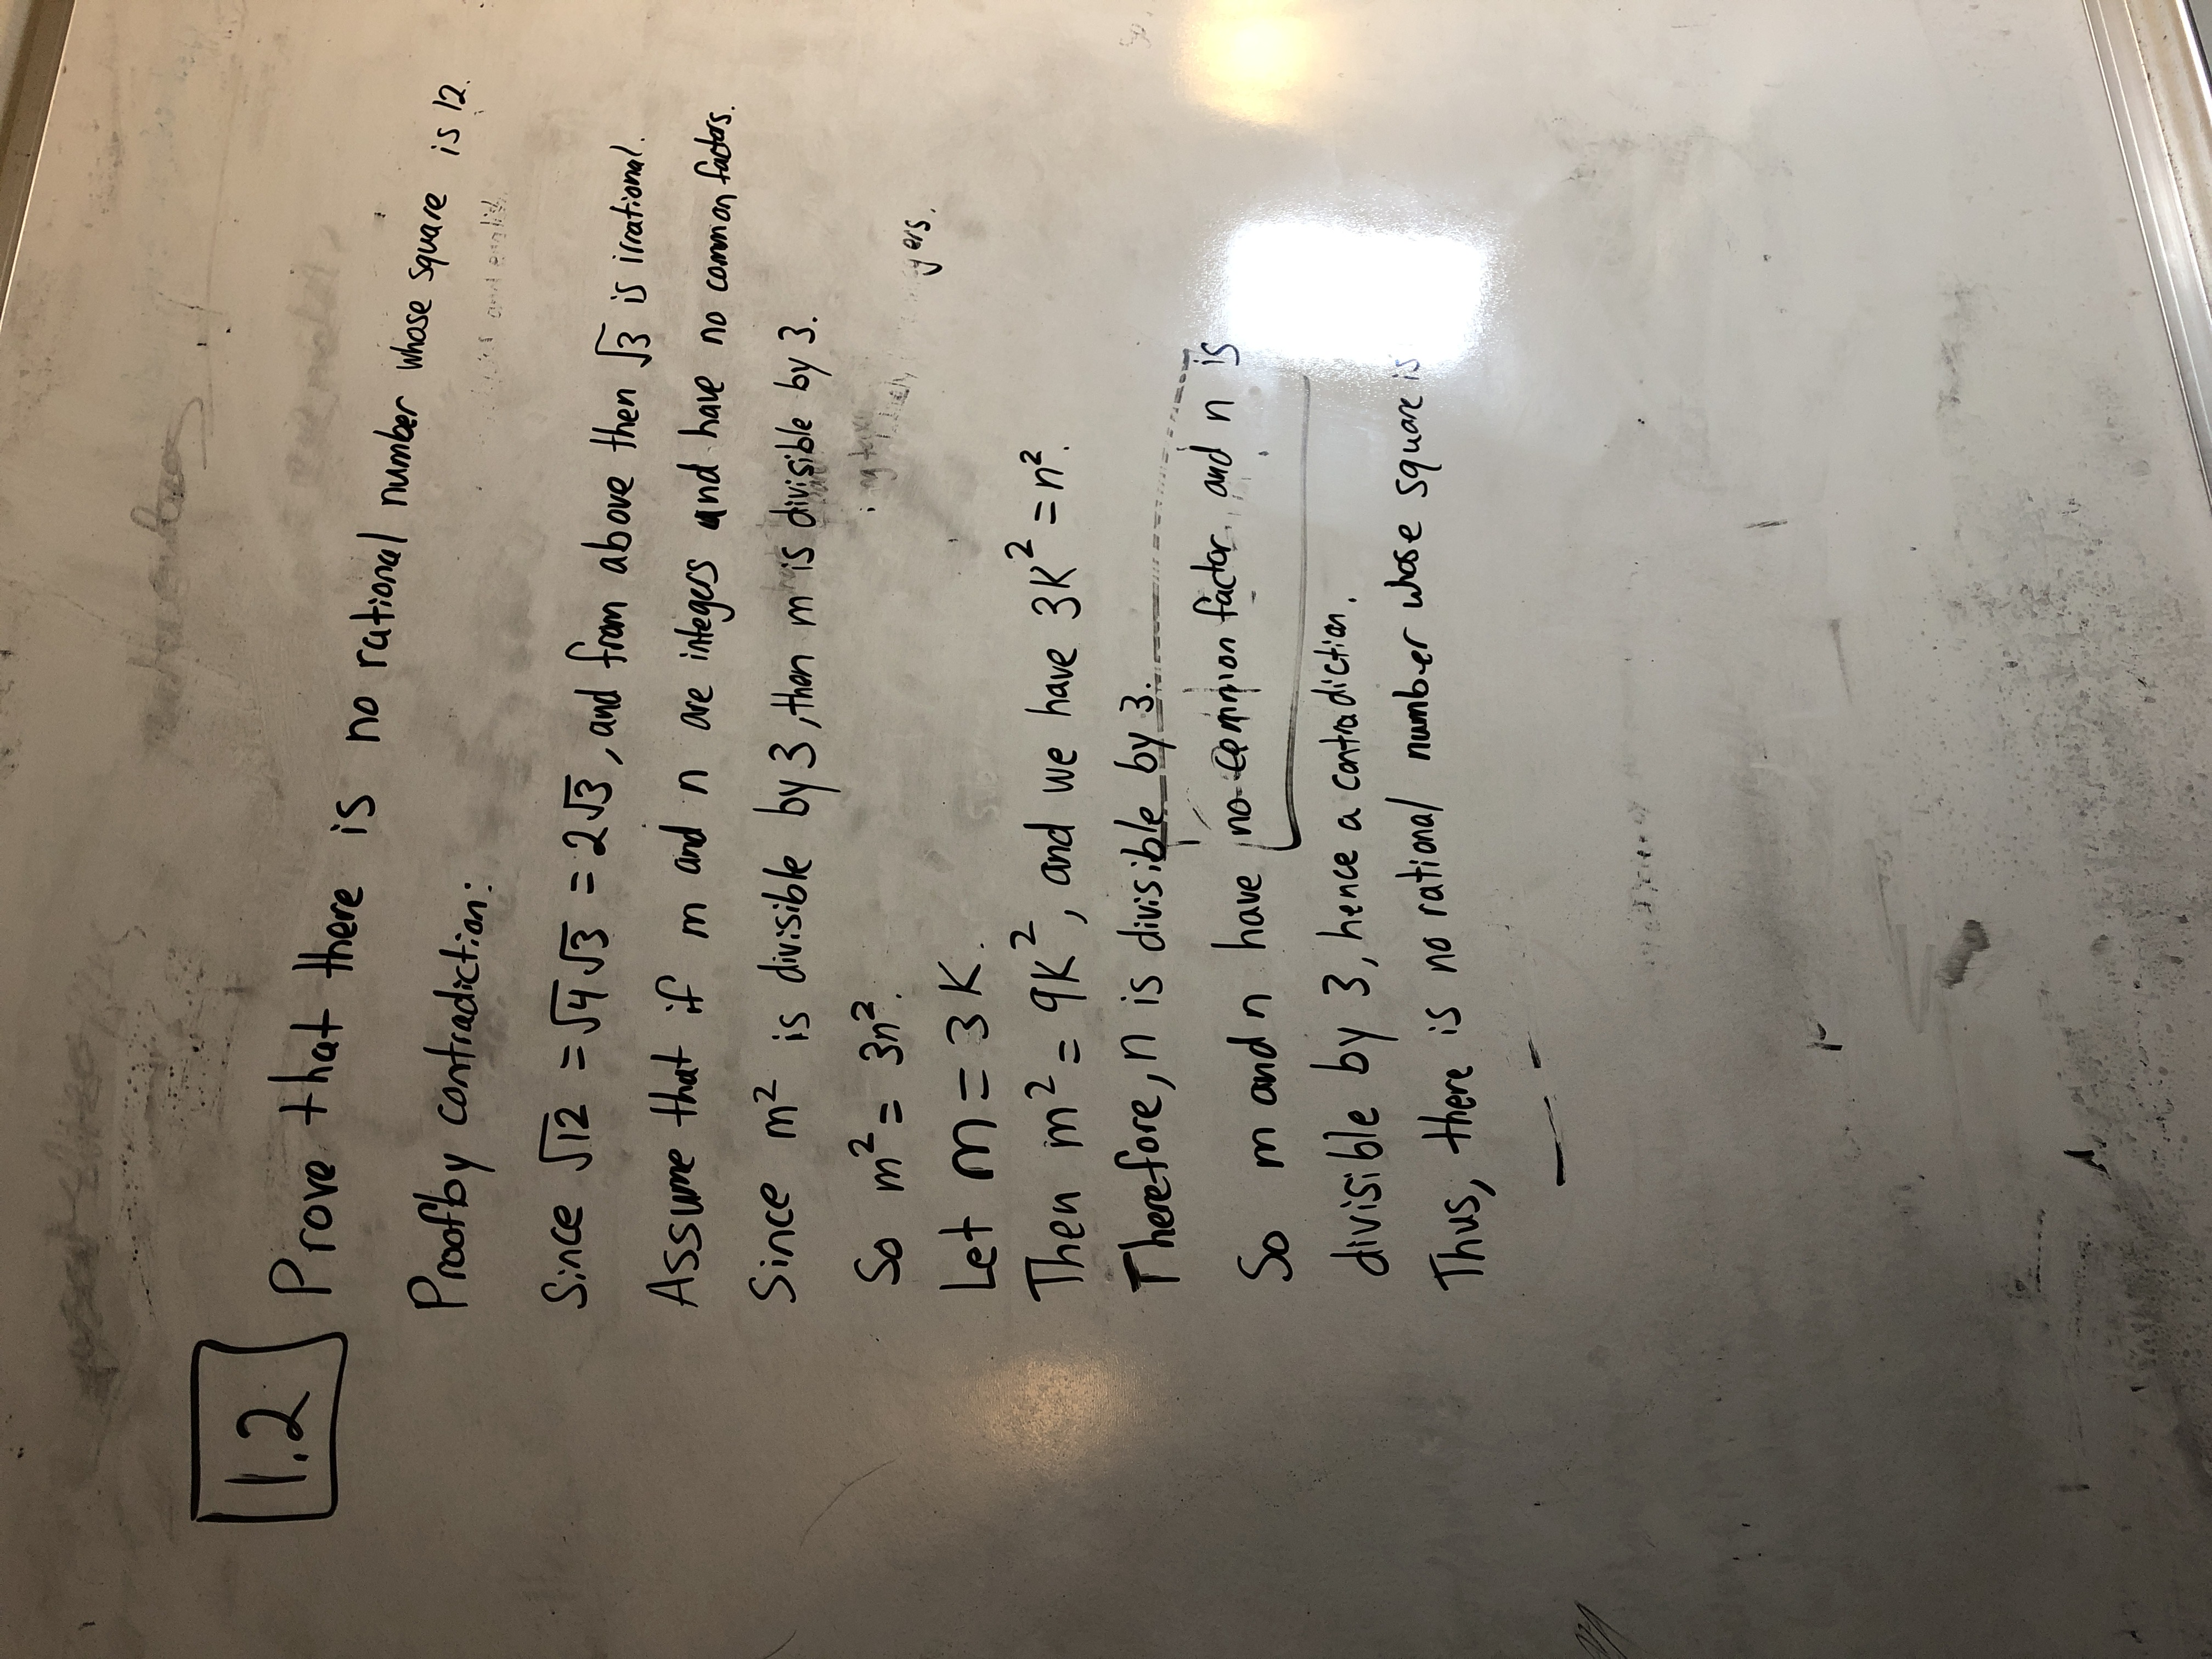
\includegraphics[angle=, origin=c,width=5 in]{Figures/IMG_1077.JPG}
\caption{Placeholder for my proofs} \label{fig:Euler_pic}\end{center}\end{figure} 

\subsection*{Baby Rudin Independent Study: Problem 10}
Suppose $z= a+bi$, $w=u+iv,$ and $a= \left(\frac{|w|+u}{2} \right)^\frac{1}{2}, b= \left(\frac{|w|-u}{2} \right)^\frac{1}{2}.$ \\ 
Prove that $z^2 =w$ if $v\geq 0$ and that $(\bar{z})^2=w$ if $v \leq 0.$ Conclude that every complex number (with one exception!) has two complex square roots. \\ 
Proof: \\ 
$z^2= (a+bi)^2= (a^2-b^2)+2abi.$\\
So, $a^2-b^2= \frac{|w|+u}{2}- \frac{|w|-u}{2}=u.$\\
Since $(xy)^\frac{1}{2}= x^\frac{1}{2} y^\frac{1}{2},$ ,$2ab= 2 \left( \frac{|w|+u}{2} \frac{|w|-u}{2}\right)^\frac{1}{2}= 2 \left( \frac{|w|^2 -u^2}{4}\right)^\frac{1}{2}.$\\
Therefore, $2ab = 2 \left( \left(\frac{v}{2} \right)^2 \right)^\frac{1}{2}.$ \\ 
So, $(x^2)^\frac{1}{2} =x$ if $x \geq 0$ and $(x^2)^\frac{1}{2}= -x$ if $x \leq 0.$ 
\\Thus, 2ab=v if $v \geq 0$ and $2ab= -v$ if $v \leq 0.$ \\ 
Hence $z^2 =w$ if $v \geq 0.$ \\ 
Then plugging in b with -b, we find that $( \bar{z})^2=w$ if $v \leq 0.$ \\ 
Then plugging in b with -b , we find that $(\bar{z})^2=w $ if $v \leq 0. $ \\ 
Thus, every non-zero complex number has (at least) two complex square roots. Hence it is proved. 


\subsection*{Baby Rudin: Independent Study Problem 12}

Here as follows is a proof setting up for Cauchy Schwartz inequality. Ideally, I would like to type set theorem 1.33 for reference. 
\section*{Problem 12}
If $z_1,...,z_n$ are complex, prove that \\
\\$|z_1 +z_2 + ... +z_n| \leq |z_1| + |z_2| + ... +|z_n|.$ \\ 
Proof by induction: \\ 
Base case:
Since in Theorem 1.33, $|z+w| \leq |z|+|w|.$ \\ 
Then when n=2 $|z_1+z_2| \leq |z_1|+|z_2|$.
\\ 
Inductive Step:
\\ 
$|z_1+z_2 + ... +z_n|= |(z_1 +z_2 + ... + z_{n-1}) +z_n|.$ \\ 
$|z_1+z_2 + ... +z_n|\leq |z_1 +z_2 + ... + z_{n-1} +z_n|.$ \\ 
Hence, $|z_1+z_2 + ... +z_n| \leq |z_1| +|z_2| + ... + |z_{n-1}| +|z_n|$ is proved by induction. \\ 
\begin{figure}[ht]\begin{center}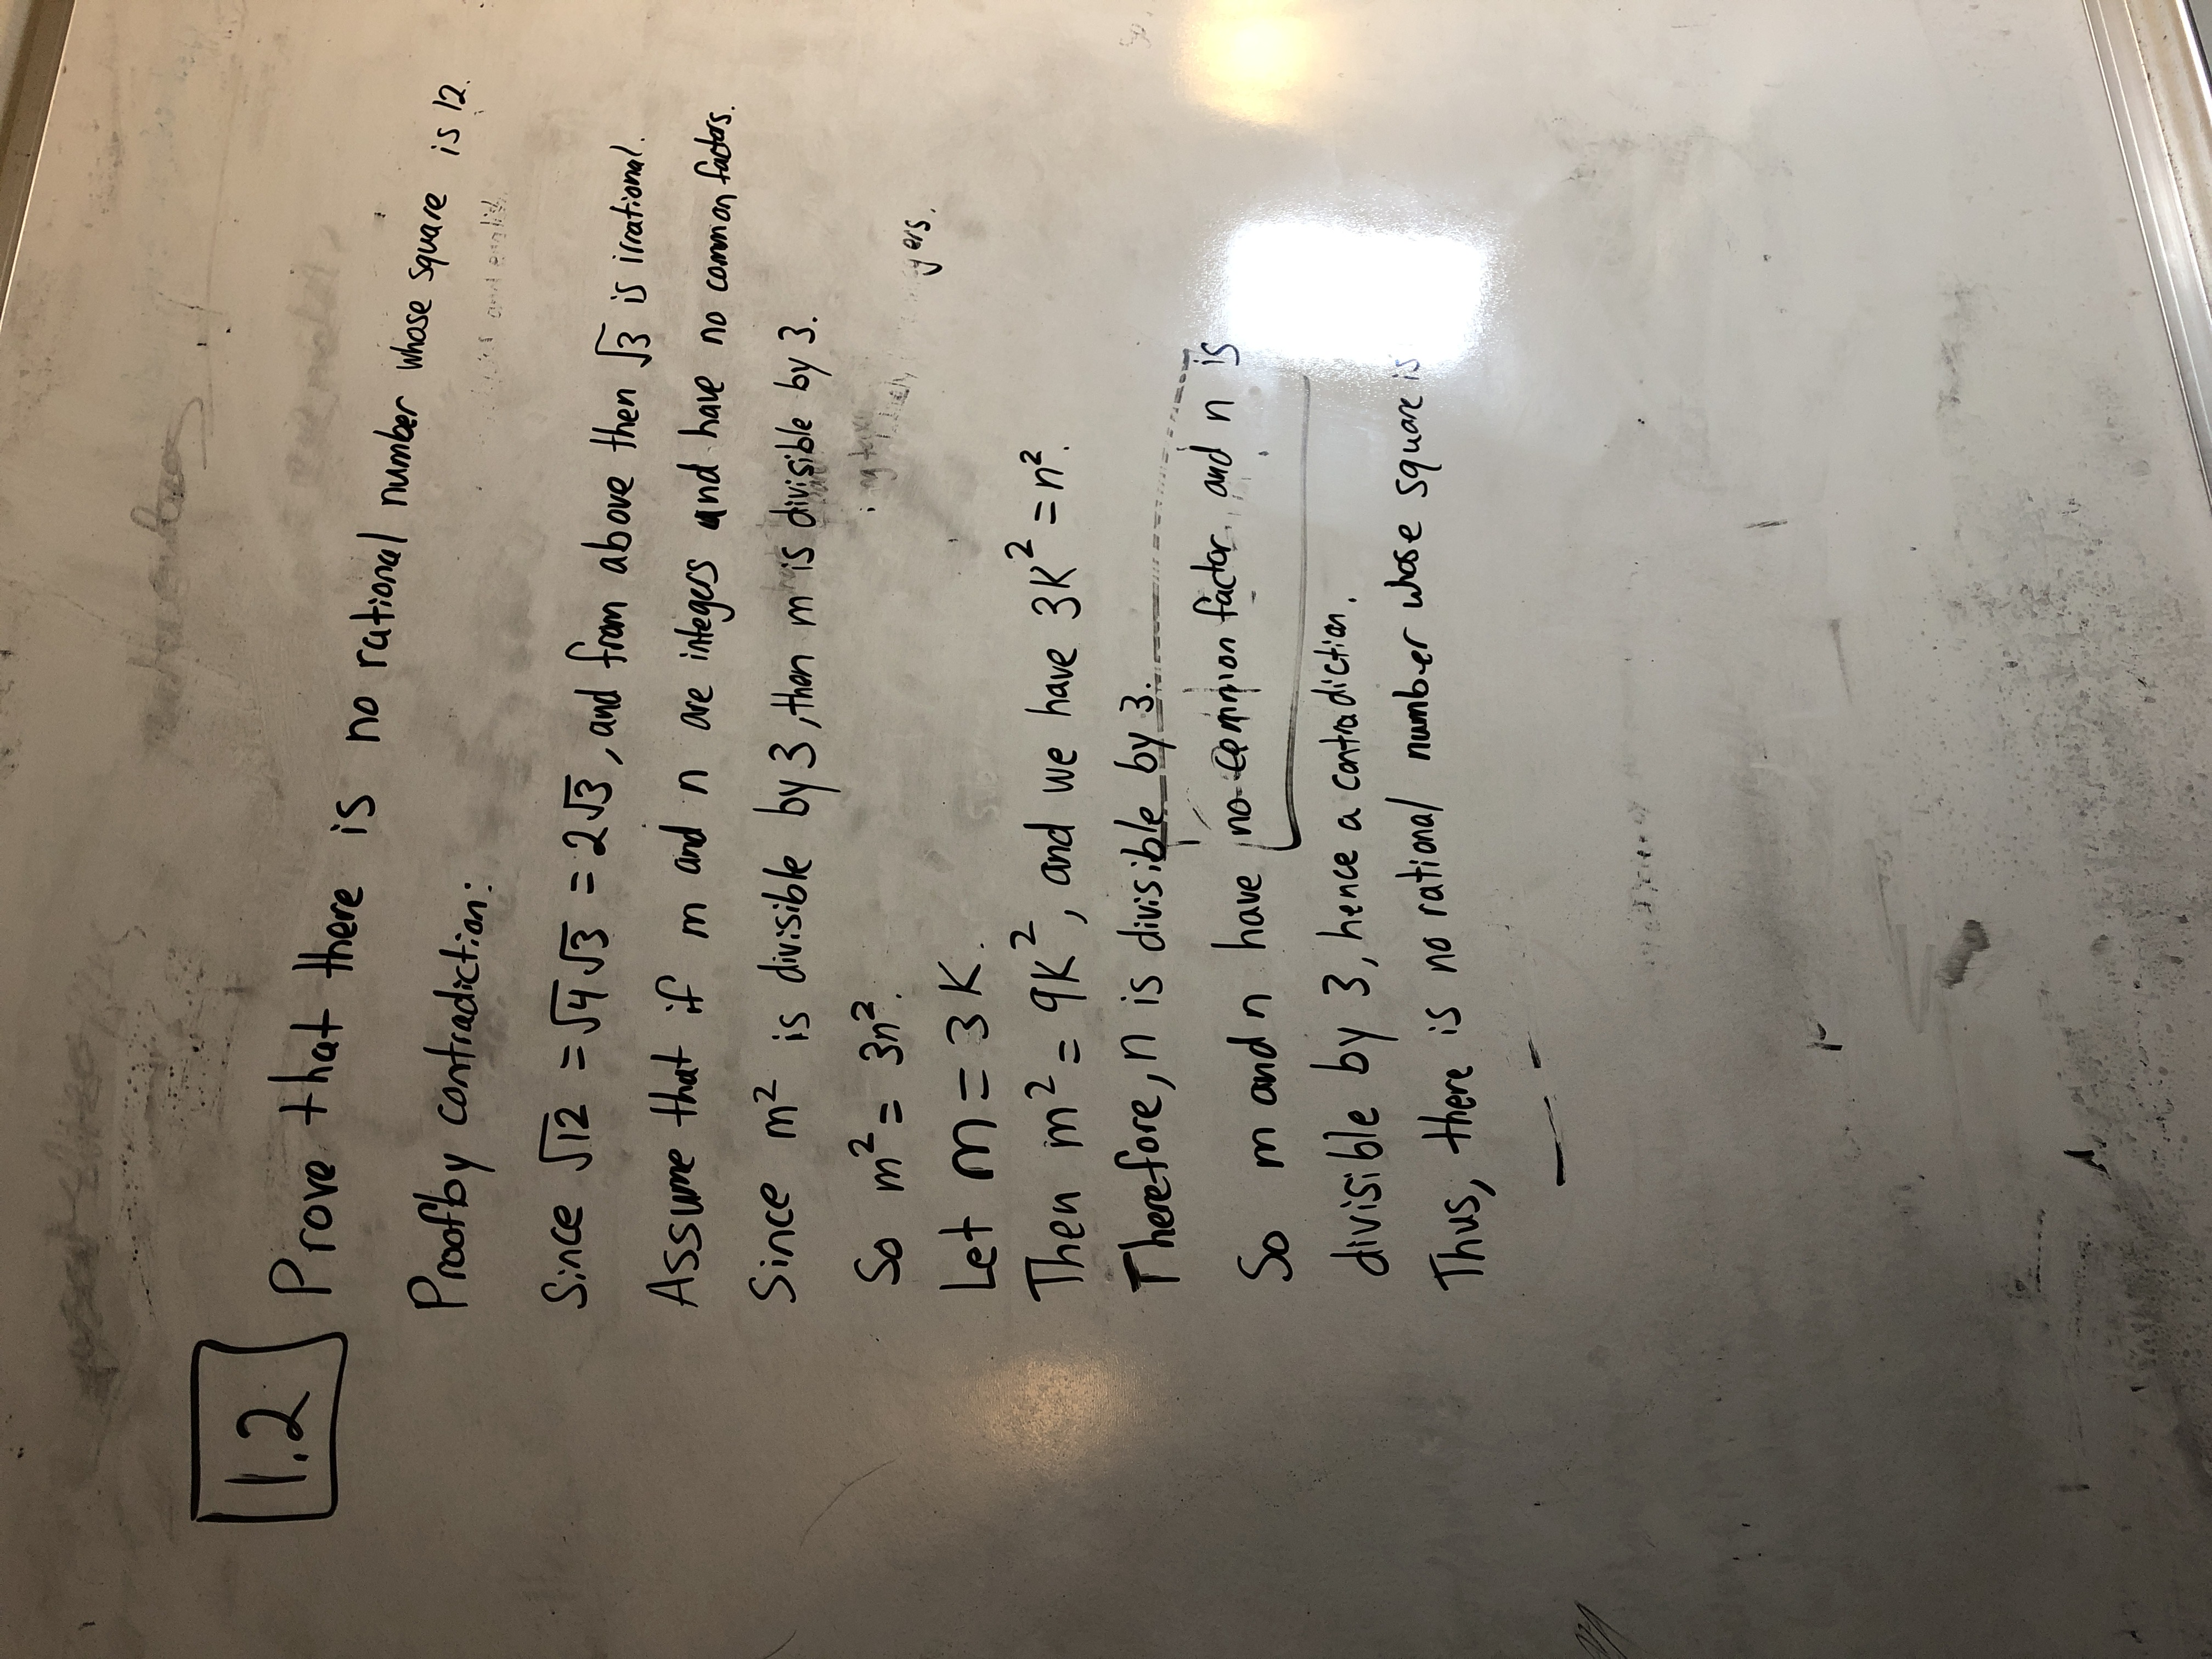
\includegraphics[angle=, origin=c,width=5 in]{Figures/IMG_1077.JPG}
\caption{Placeholder for my proofs} \label{fig:Euler_pic}\end{center}\end{figure} 

\newpage 
\subsection*{Baby Rudin Independent Study: Problem 13}
If x,y are complex, prove that $||x|-|y|| \leq|x-y|.$ \\
Proof: \\ 
Since x= x-y+y, by definition of the triangle inequality $|x| \leq |x-y|+y$, so $|x|-|y| \leq |x-y|.$ \\ 
So $|y|-|x| \leq |x-y|$. \\ 
Since $|x| - |y|$ is in the set of real numbers, then $||x|-|y|$ or $||x|-|y||= |y|-|x|.$ \\
Thus, $||x|-|y|| \leq |x-y|$. Hence it is proved. 
\begin{figure}[ht]\begin{center}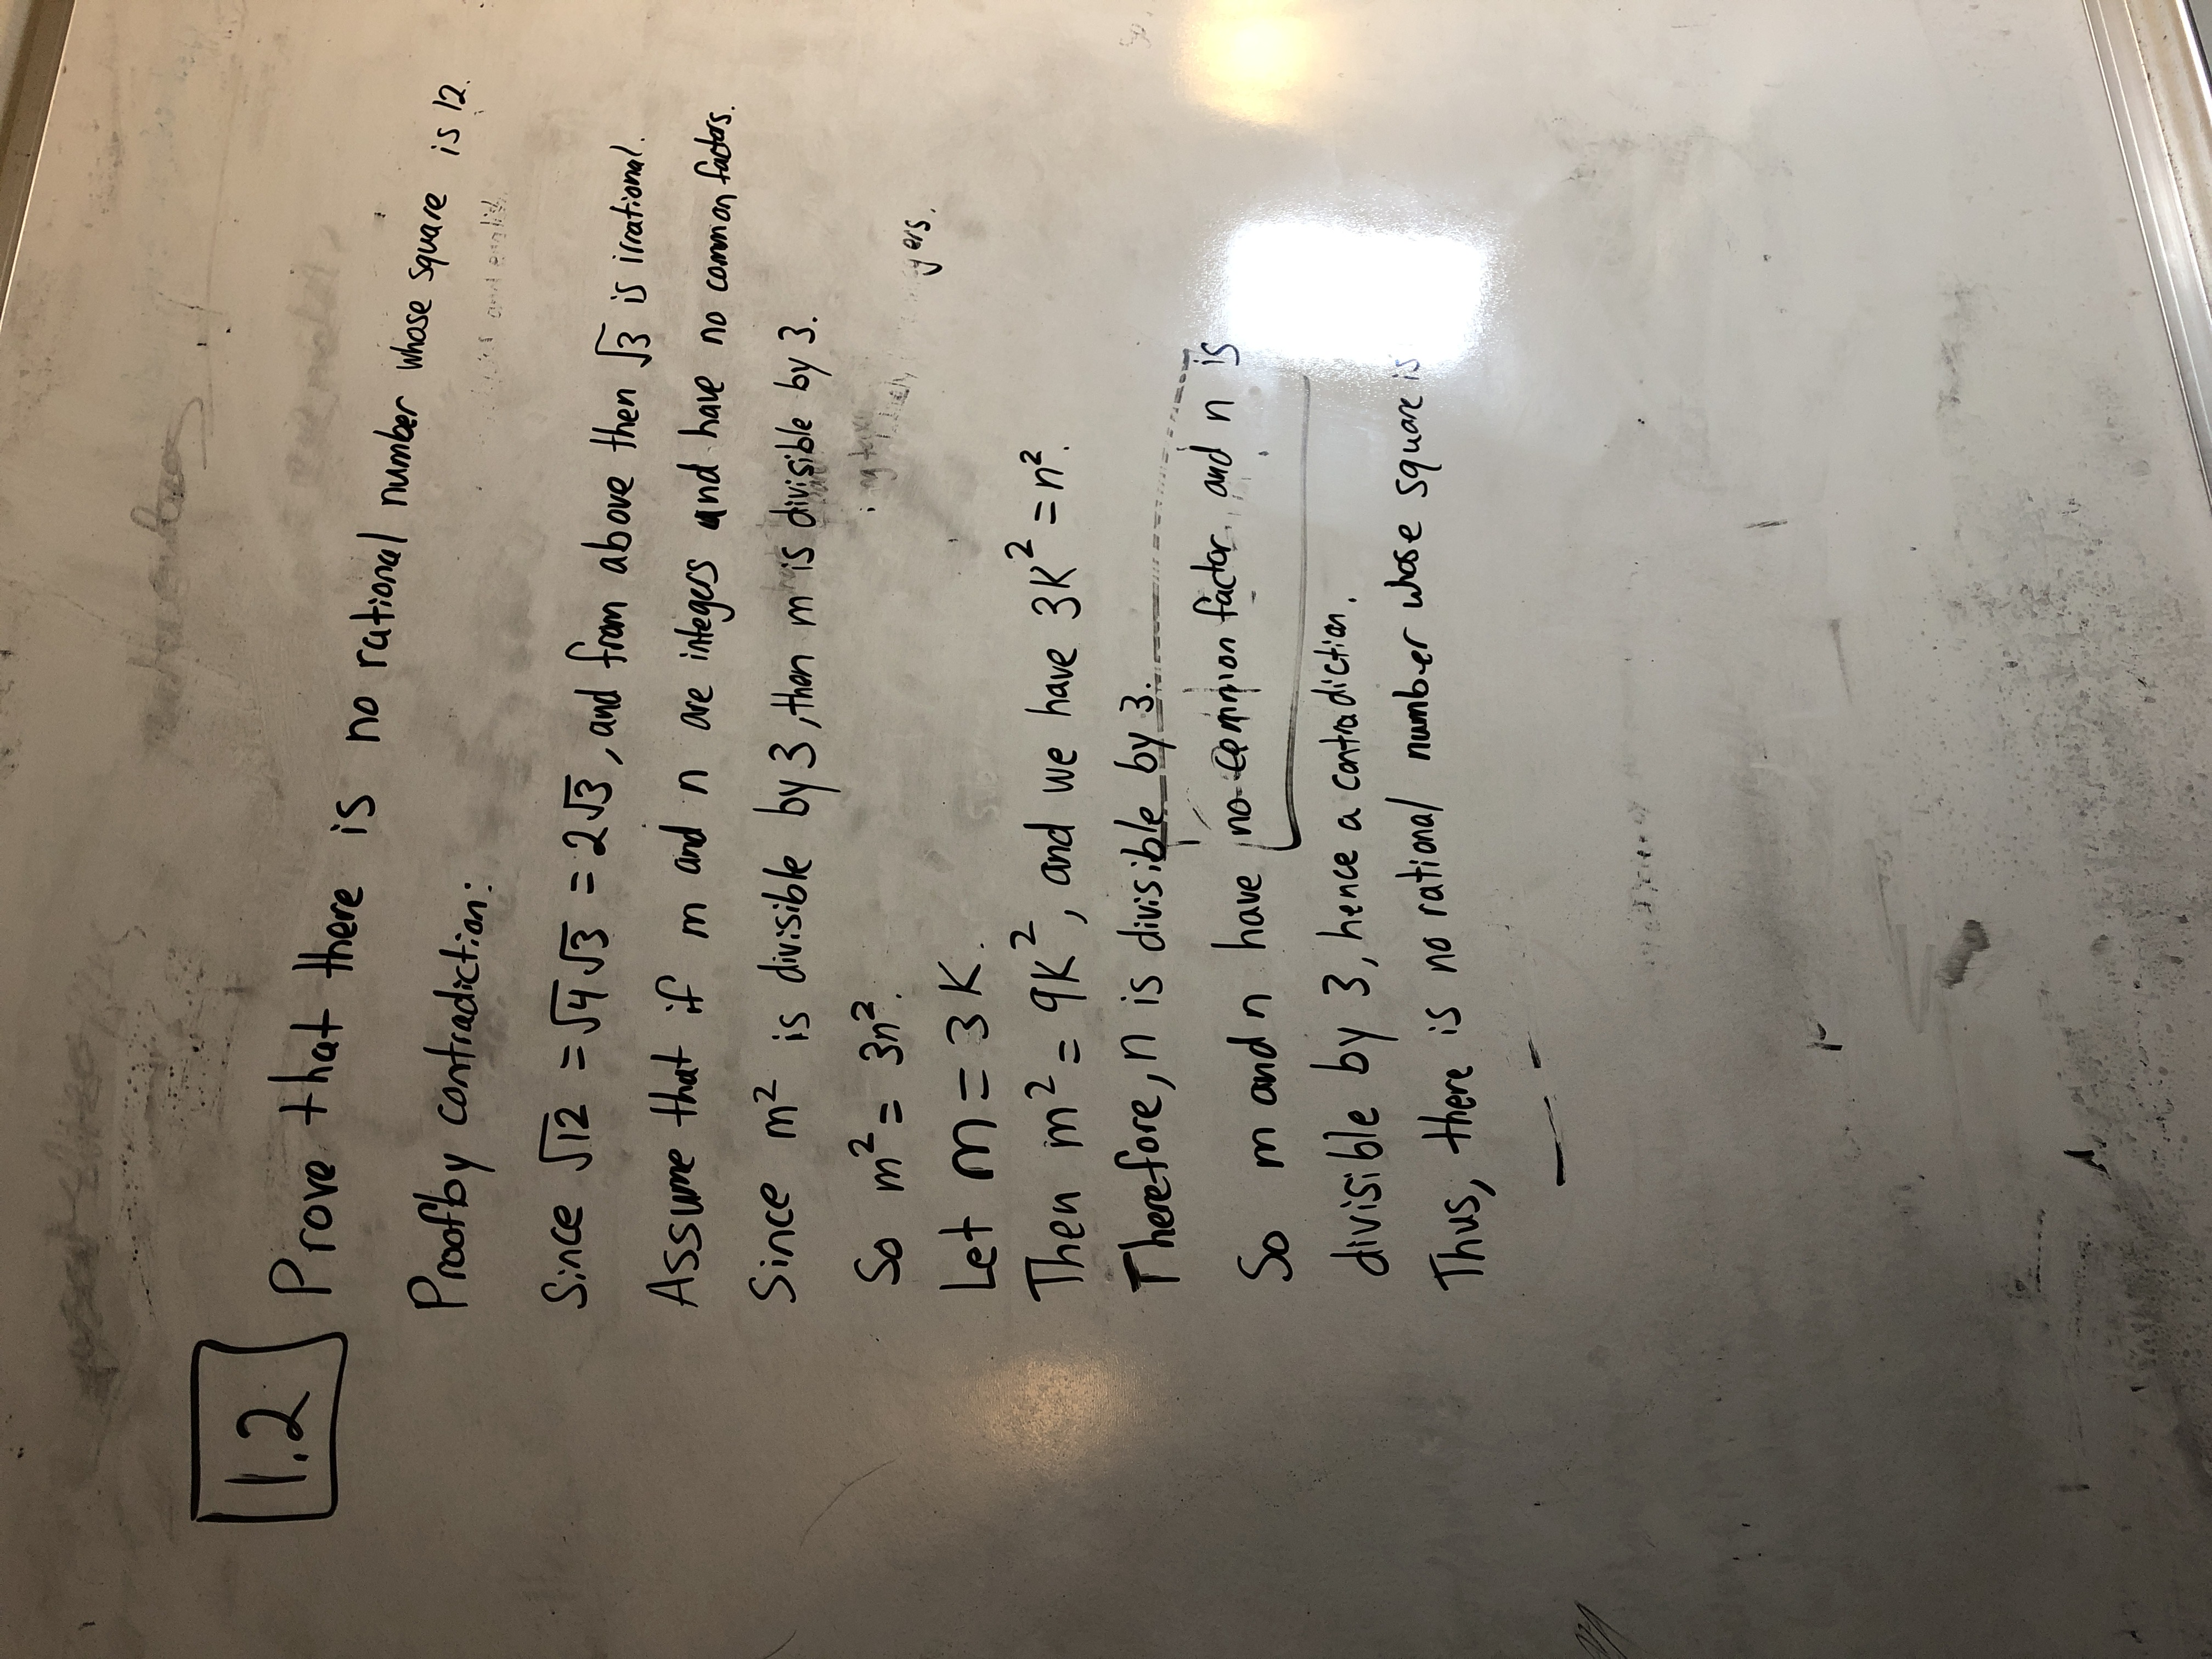
\includegraphics[angle=, origin=c,width=5 in]{Figures/IMG_1077.JPG}
\caption{Placeholder for my proofs} \label{fig:Euler_pic}\end{center}\end{figure} 
\newpage
Grade Problem 2.1 and 2.3.  
\subsection*{Problem 1.16}
Suppose $k \geq 3, x,y,\in R^k, |x-y|=d>0,$ and $r>0.$ \\ Prove: 
(a)If $2r>d$, there are infinitely many z $\in R^k$ such that $|z-x|=|z-y|=r.$ \\ 
(b) If $2r = d,$ there is exactly one such z. \\ 
(c) If $2r < d,$ there is no such z. \\ 
How must these statements be modified if k is 2 or 1? \\ 
Proof: \\ 
(a) Let w be any vector where: \\ 
$w \cdot (x-y)=0,$ \\ 
$|w|^2 = r^2 - \frac{d^2}{4}.$ \\ 
%From linear algebra it is known that all but one of the components of a solution w of the first equation can be arbitrary. \\
%The remaining component is then uniquely determined.Also, if w is any non-zero solution of the first equation, there is a unique positive number t such that tw satisfies both equations. (For example, if $\x_1 \neq y_1, $ the first equation is satisfied whenever $z_1 =\frac{z_2(x_2-y_2)+ \dots + z_k(x_k-y_k)}{y_1-x_1}.$ \\ 
%If $(z_1, z_2, \dots, z_k)$ satisfies this equation, so does $(tz_1, tz_2, \dots tz_k)$ for any real number t.) Since at least two of these components can vary independently, we can find a solution with these components having any prescribed ratio. This ratio does not change when we multiply by the positive number t to obtain a solution of both equations. 
Since there are infinitely many ratios, there are infinitely many distinct solutions. For each such solution w the vector z= $\frac{1}{2}x + \frac{1}{2}y + w$ is a solution of the required equation. For \\
$|z-x|^2= |\frac{y-x}{2}+w|^2$ \\ 
$|z-x|^2= |\frac{y-x}{2}|^2 +2w \cdot \frac{x-y}{2}+|w|^2$ \\ 
$|z-x|^2= \frac{d^2}{4}+0 +r^2 -\frac{d^2}{4}$ \\ 
$|z-x|^2 = r^2,$ \\
$|z-y|^2=r^2.$ \\ 
(b) The triangle inequality proof demonstrates that $2r=d$ only is true if it is equal in the Schwartz inequality.\\ Then one of the two vectors is a scalar multiple of the other one.\\ Furthermore, the scalar must be nonnegative. 
\\Next, $|x-y|=d=|x-z|+|z-y|.$ \\ 
Hence, there is a nonnegative scalar t such that $x-z =t(z-y).$ \\ 
So, the above equation leads to t=1. \\ 
So z is uniquely determined as $z= \frac{x+y}{2}.$ \\ 
(c) The triangle inequality is contradicted if z=$2r<d$. Then we would have $|x-y|=d>2r =|x-z|+|z-y|.$ When k=2, there are exactly 2 solutions when $2r>d$. When k=1, there are no solutions when $2r>d$. \\ 

\begin{figure}[ht]\begin{center}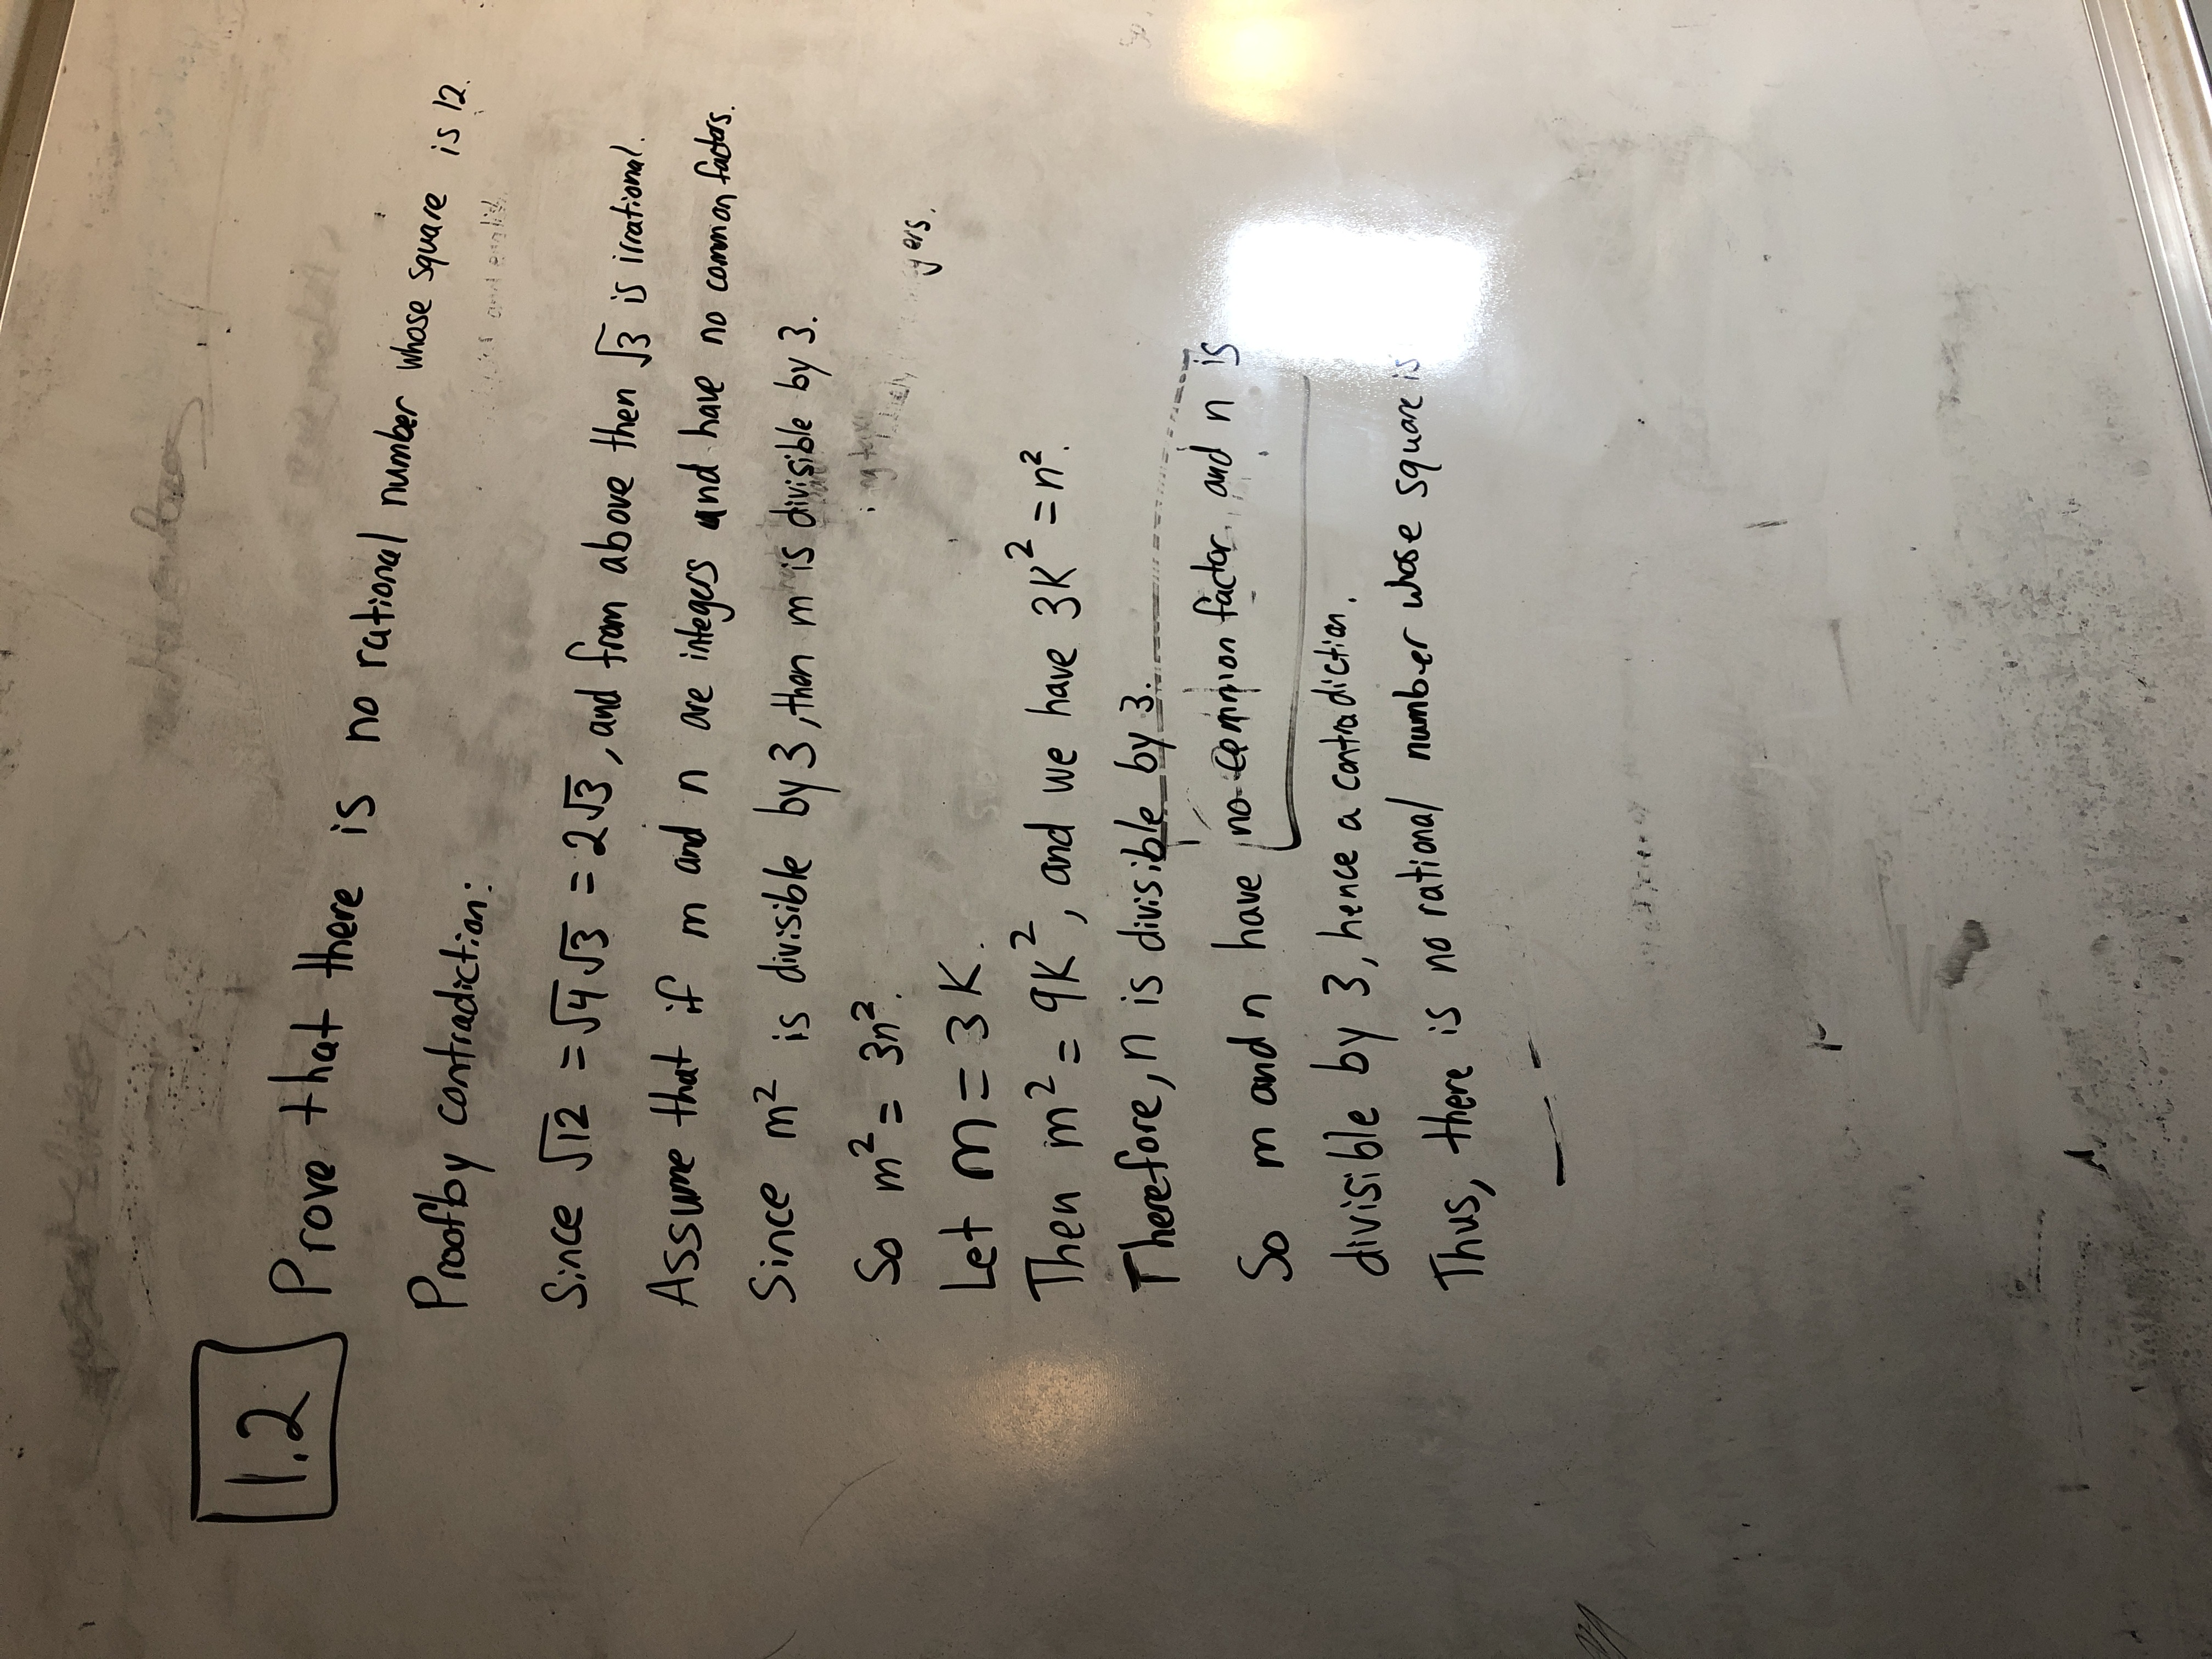
\includegraphics[angle=, origin=c,width=5 in]{Figures/IMG_1077.JPG}
\caption{Placeholder for my proofs} \label{fig:Euler_pic}\end{center}\end{figure} 
\newpage
\subsection{Problem 1.18}
If $k \geq 2$ and $x \in R^k,$ prove that there exists $y \in R^k$ such that $y \neq 0$ but $x \cdot y =0.$ Is this also true if k=1? \\ 
Proof: \\ 
If x has any components equal to 0, then y can be taken to have the corresponding components equal to 1 and all others equal to 0.\\
If all the components of x are nonzero, y can be taken as $-x_2,x_1,0, \dots,0).$ \\
Since the product of two nonzero real numbers is nonzero then this is not true when k=1, \\ 
\\
\begin{figure}[ht]\begin{center}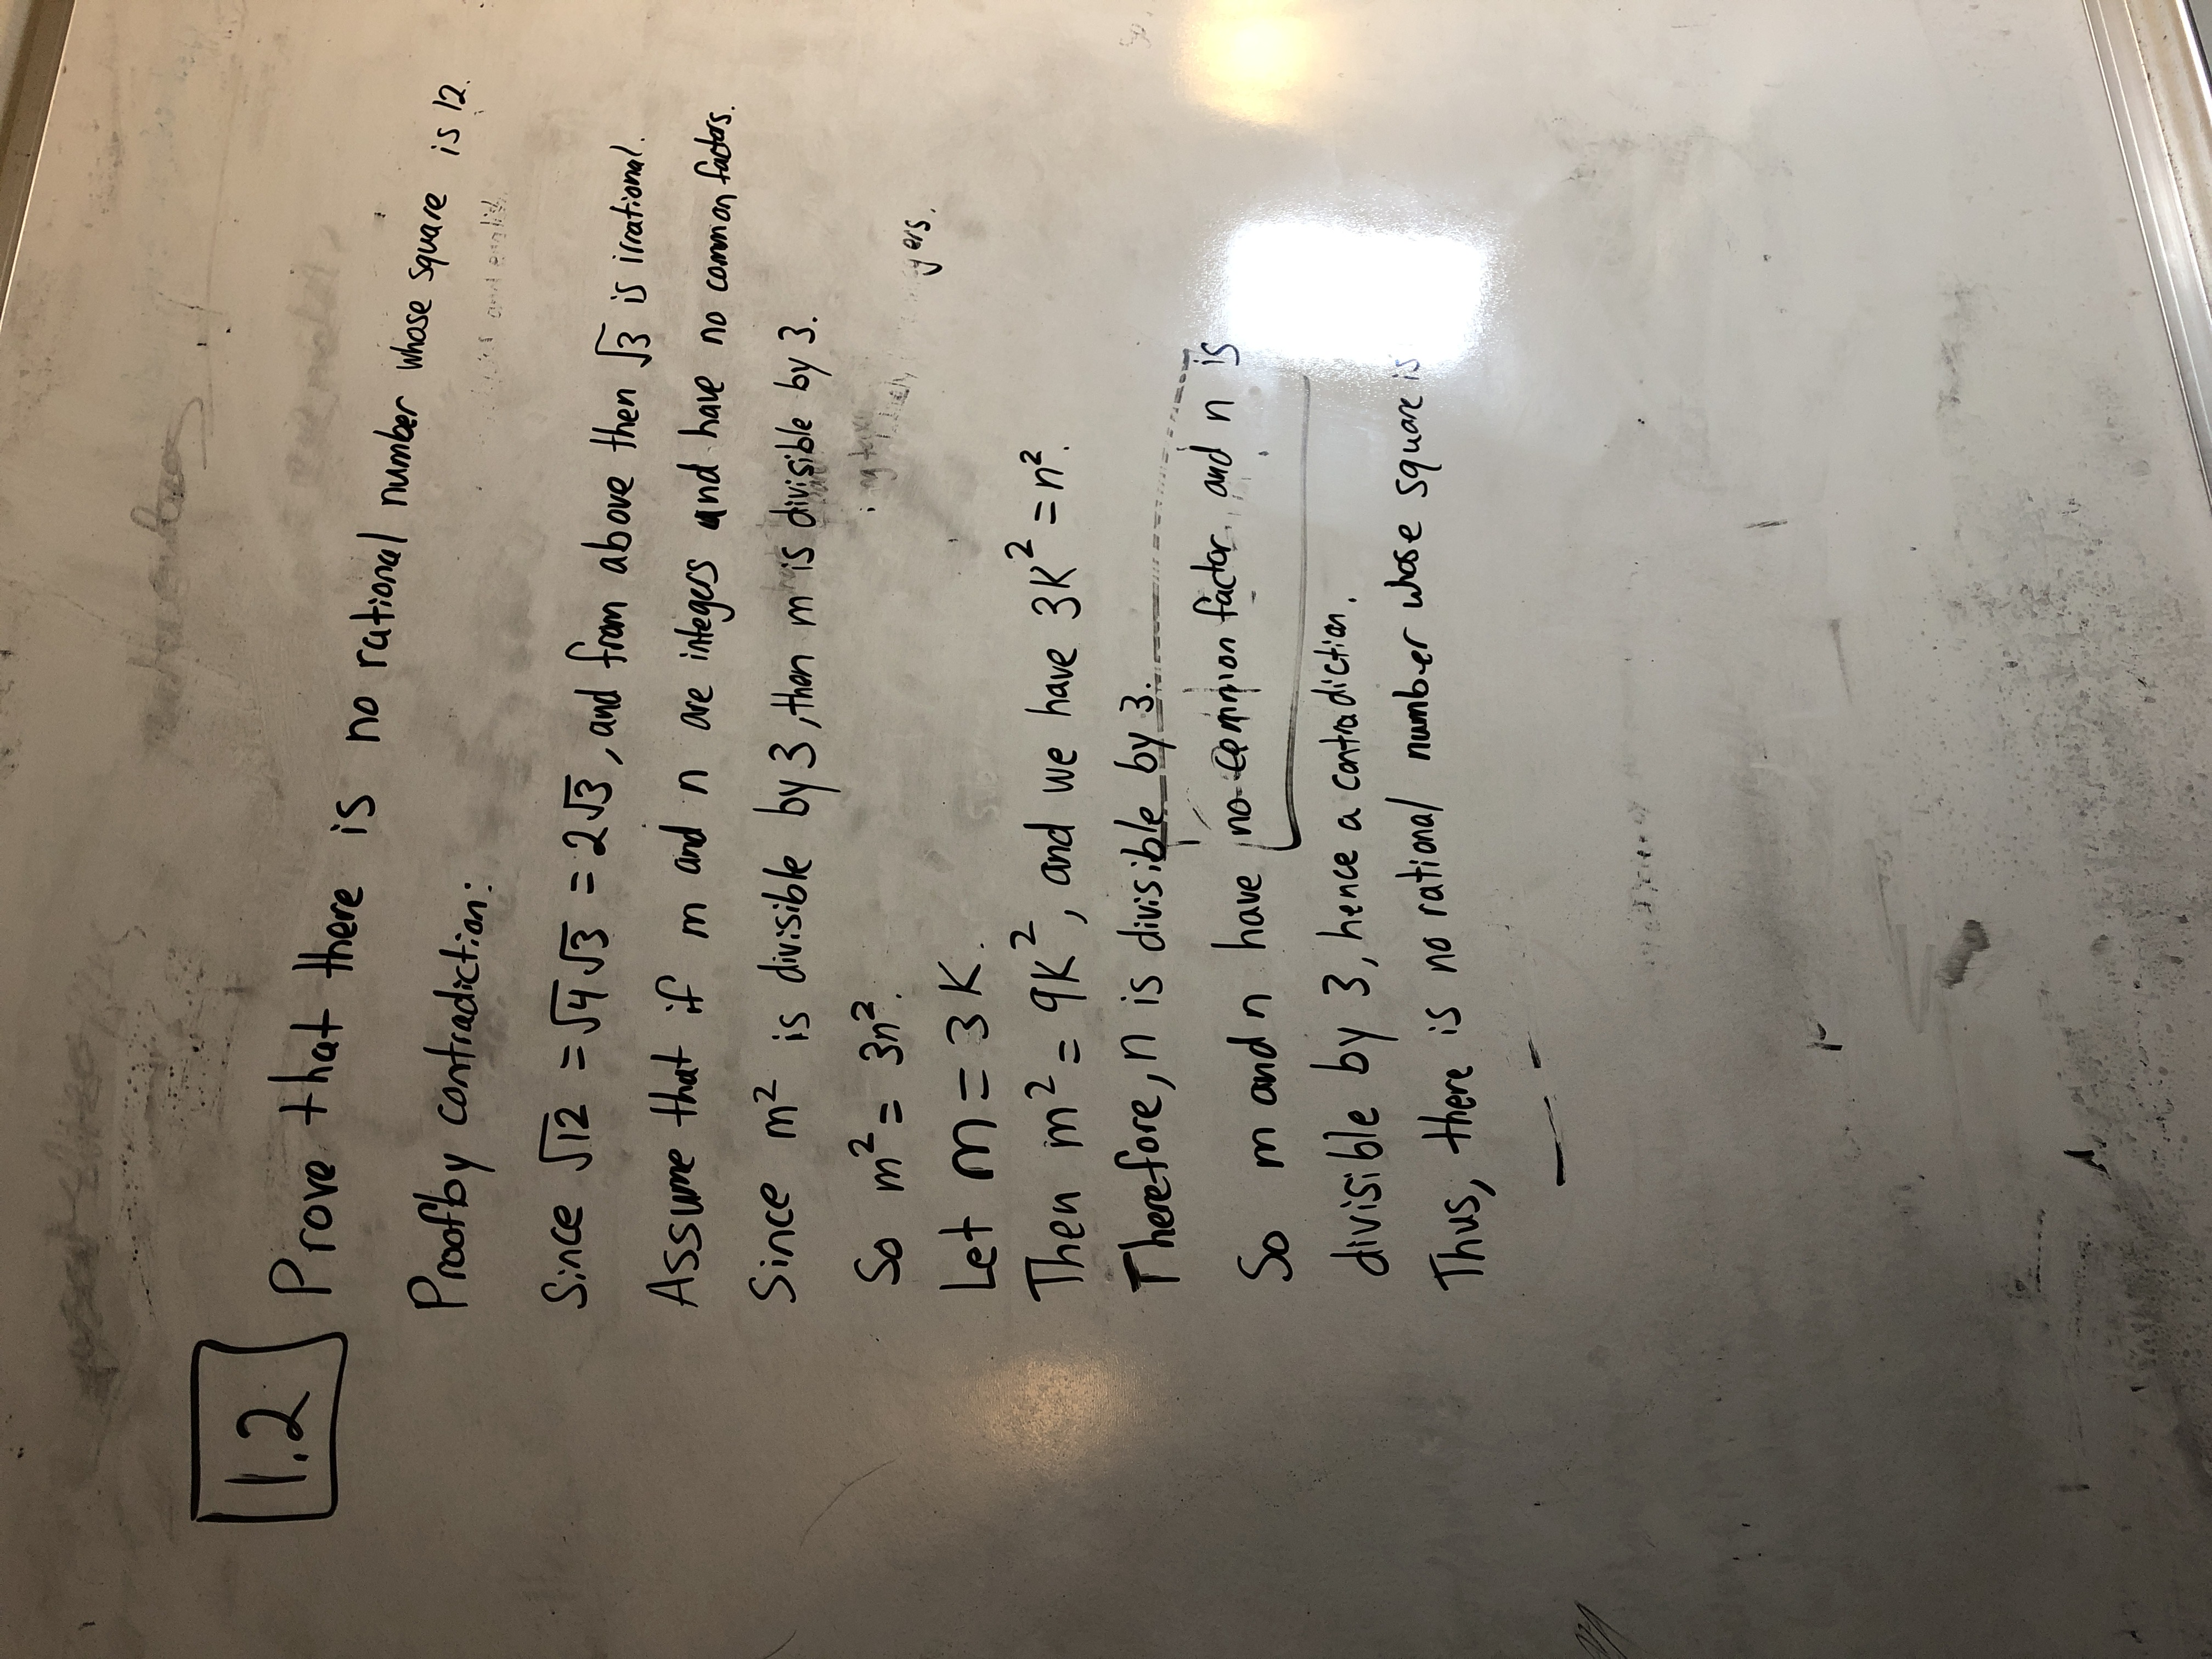
\includegraphics[angle=, origin=c,width=5 in]{Figures/IMG_1077.JPG}
\caption{Placeholder for my proofs} \label{fig:Euler_pic}\end{center}\end{figure} 



\section{Problem 2.1}
Prove that the empty set is a subset of every set. 
\\
Proof:\\ 
Let $\emptyset$ be the empty set. \\ 
Let E be every set. \\ 
Suppose $x \in \emptyset.$ \\ 
Then $x \in E.$ \\ 
Since $\emptyset$ cannot contain any elements, $x \in \emptyset$ is false. \\ 
So, $x \in E$ is true. \\ 
Thus, $\emptyset \subset E.$
\\

\begin{figure}[h]\begin{center}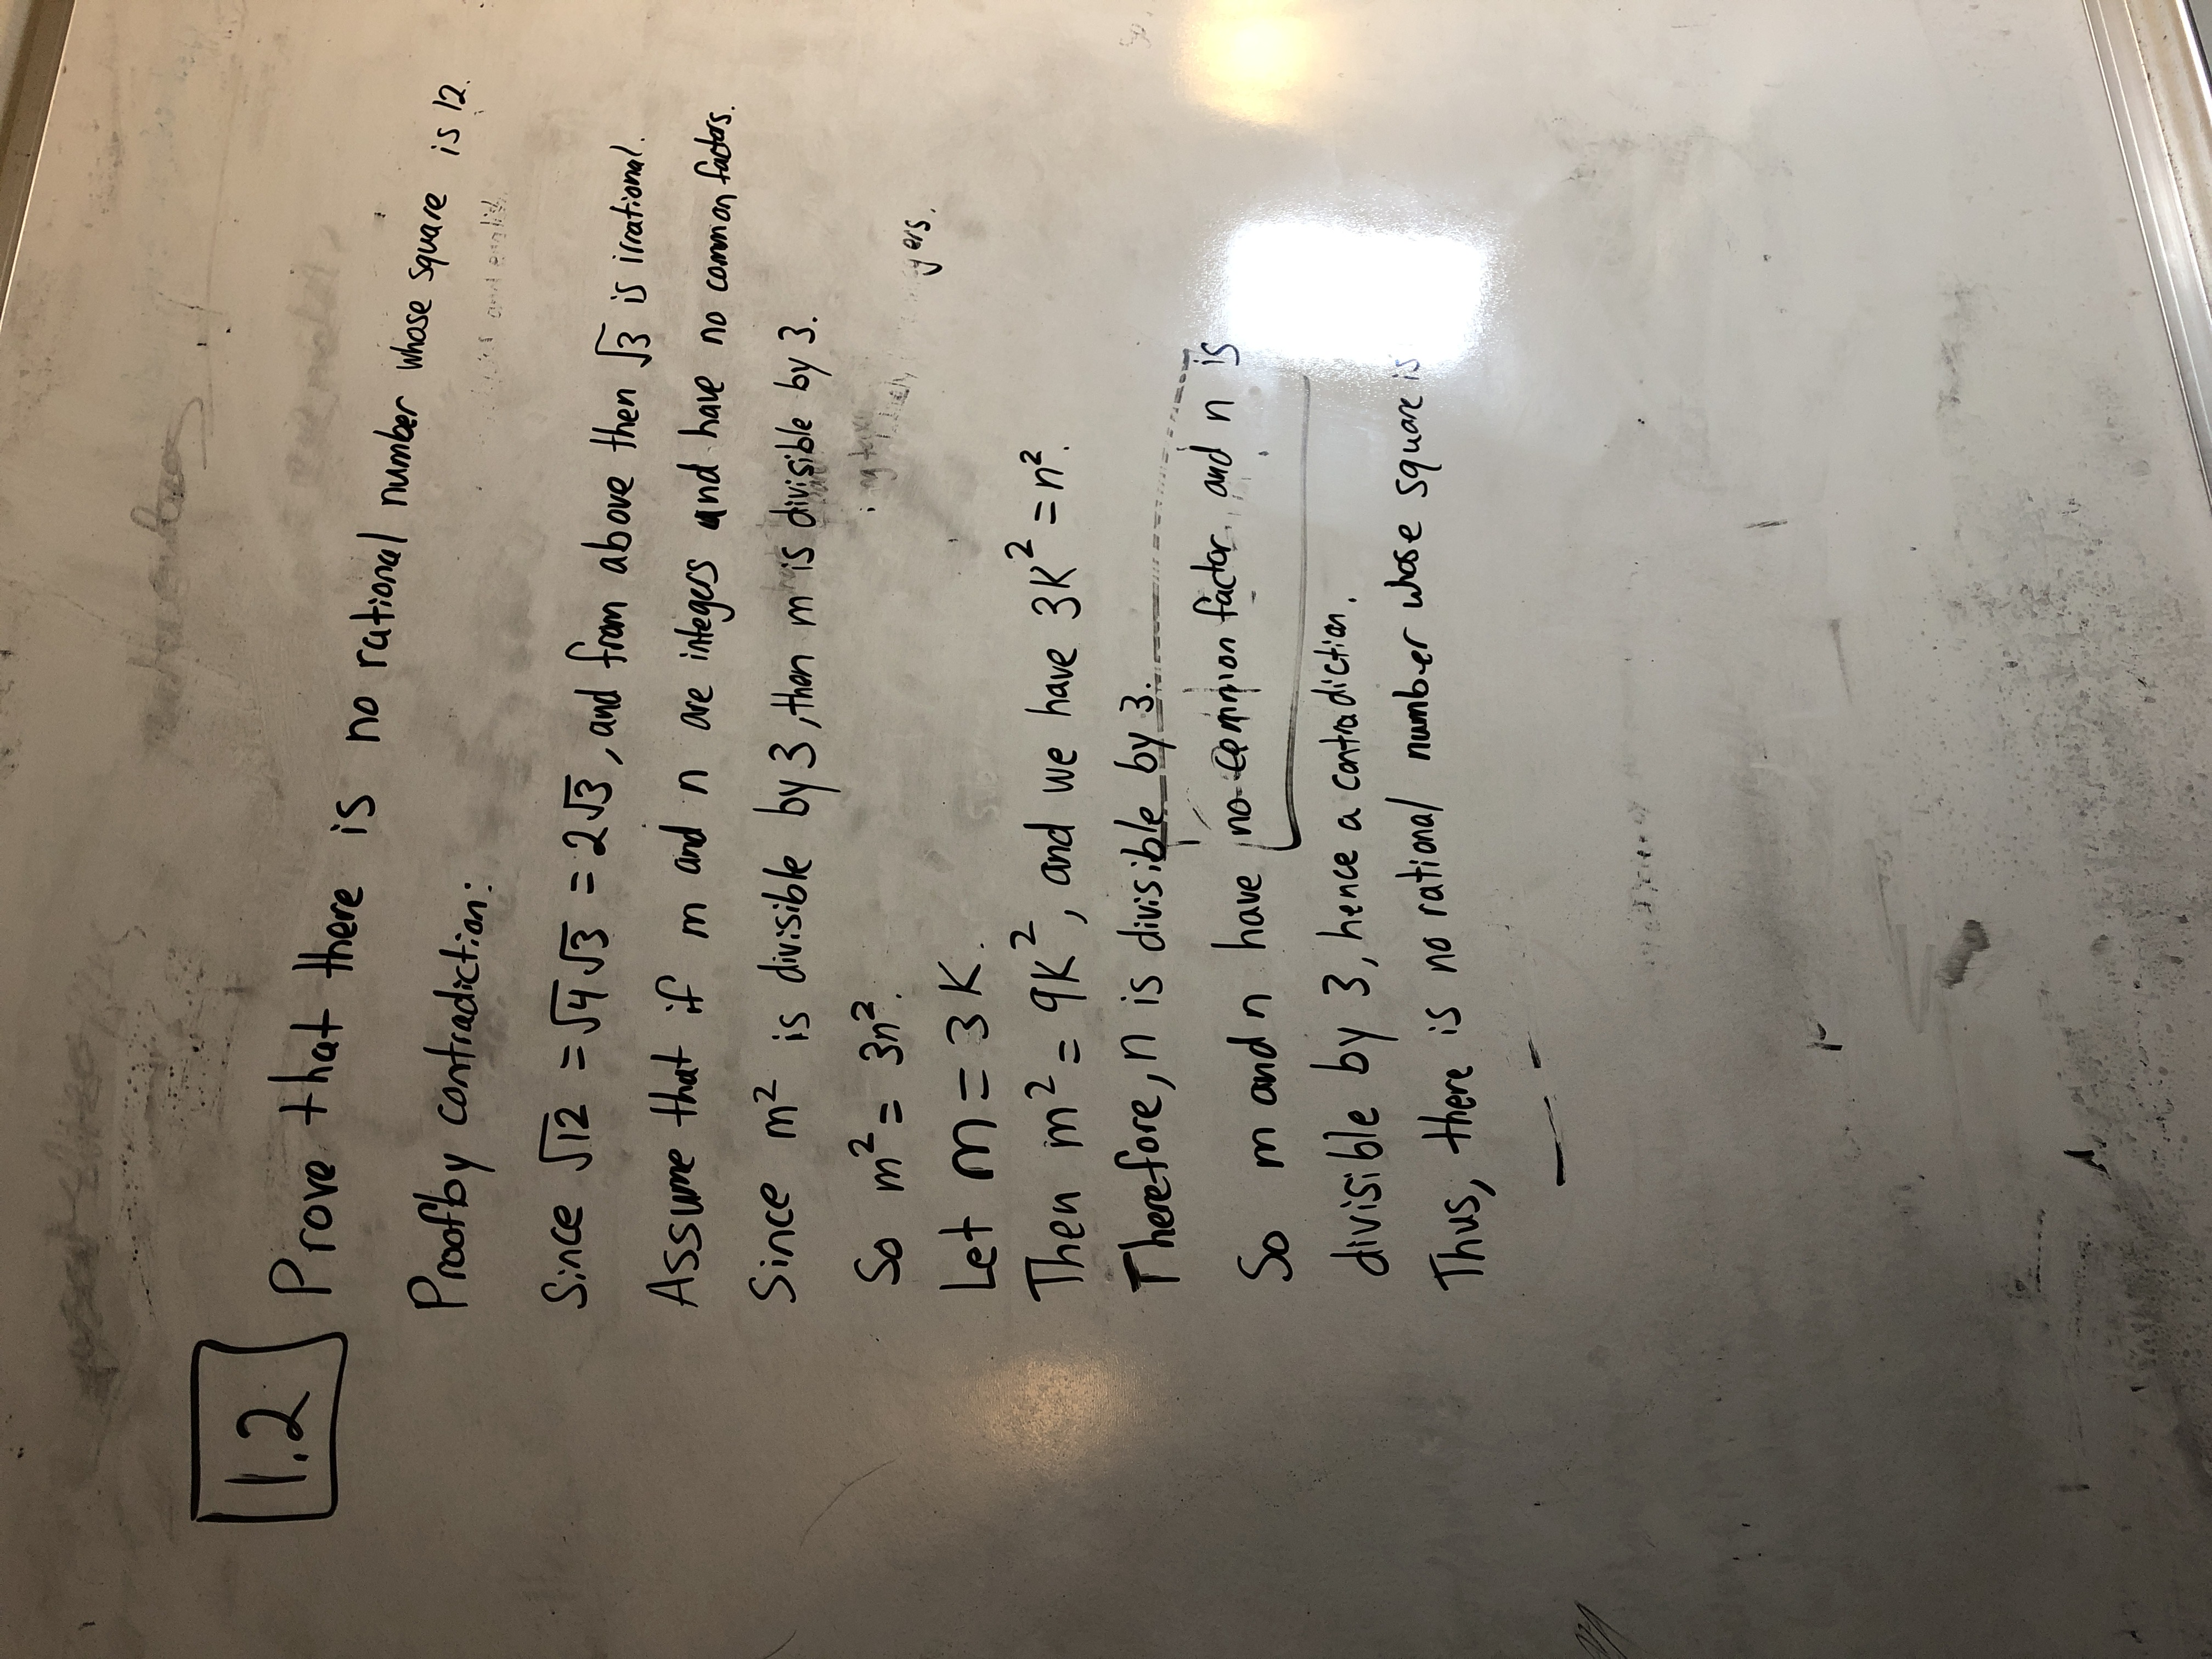
\includegraphics[angle=, origin=c,width=5 in]{Figures/IMG_1077.JPG}
\caption{Placeholder for my proofs} \label{fig:Euler_pic}\end{center}\end{figure} 
\newpage
\subsection{Problem 2.2}
A complex number z is said to be algebraic if there are integers $a_0, \dots, a_n,$ not all zero, such that $a_0 z^n + a_1 z^{n-1}+ \dots + a_n=0.$ \\ 
\\
Prove that the set of all algebraic numbers is countable. Hint: For every positive integer N there are only finitely many equations with $n+|a_0|+|a_1| + \dots |a_n|= N.$\\ 
\\
Proof:\\ 
Let $A_n$ be the set of integers $a_0 z^n + a_1 z^(n-1)+ \dots + a_n=0.$ \\ 
Each equation has finitely many equations that satisfy this condition. \\ 
By Theorem 2.12's Corollary, Suppose A is at most countable, and, for every $\alpha \in A, B_\alpha$is at most countable. Put T= $ \cup_{\alpha \in A}B_\alpha.$ Then T is at most countable. For T is equivalent to a subset of S=$\cup_{n=1}^\infty E_n$ then the set of algebraic numbers, $\cup_{n=2}^\infty A_N$, is at most countable. \\ 
Since the entirety of the rational numbers, Q, are algebraic, then the set of all algebraic numbers is countable. 


\begin{figure}[ht]\begin{center}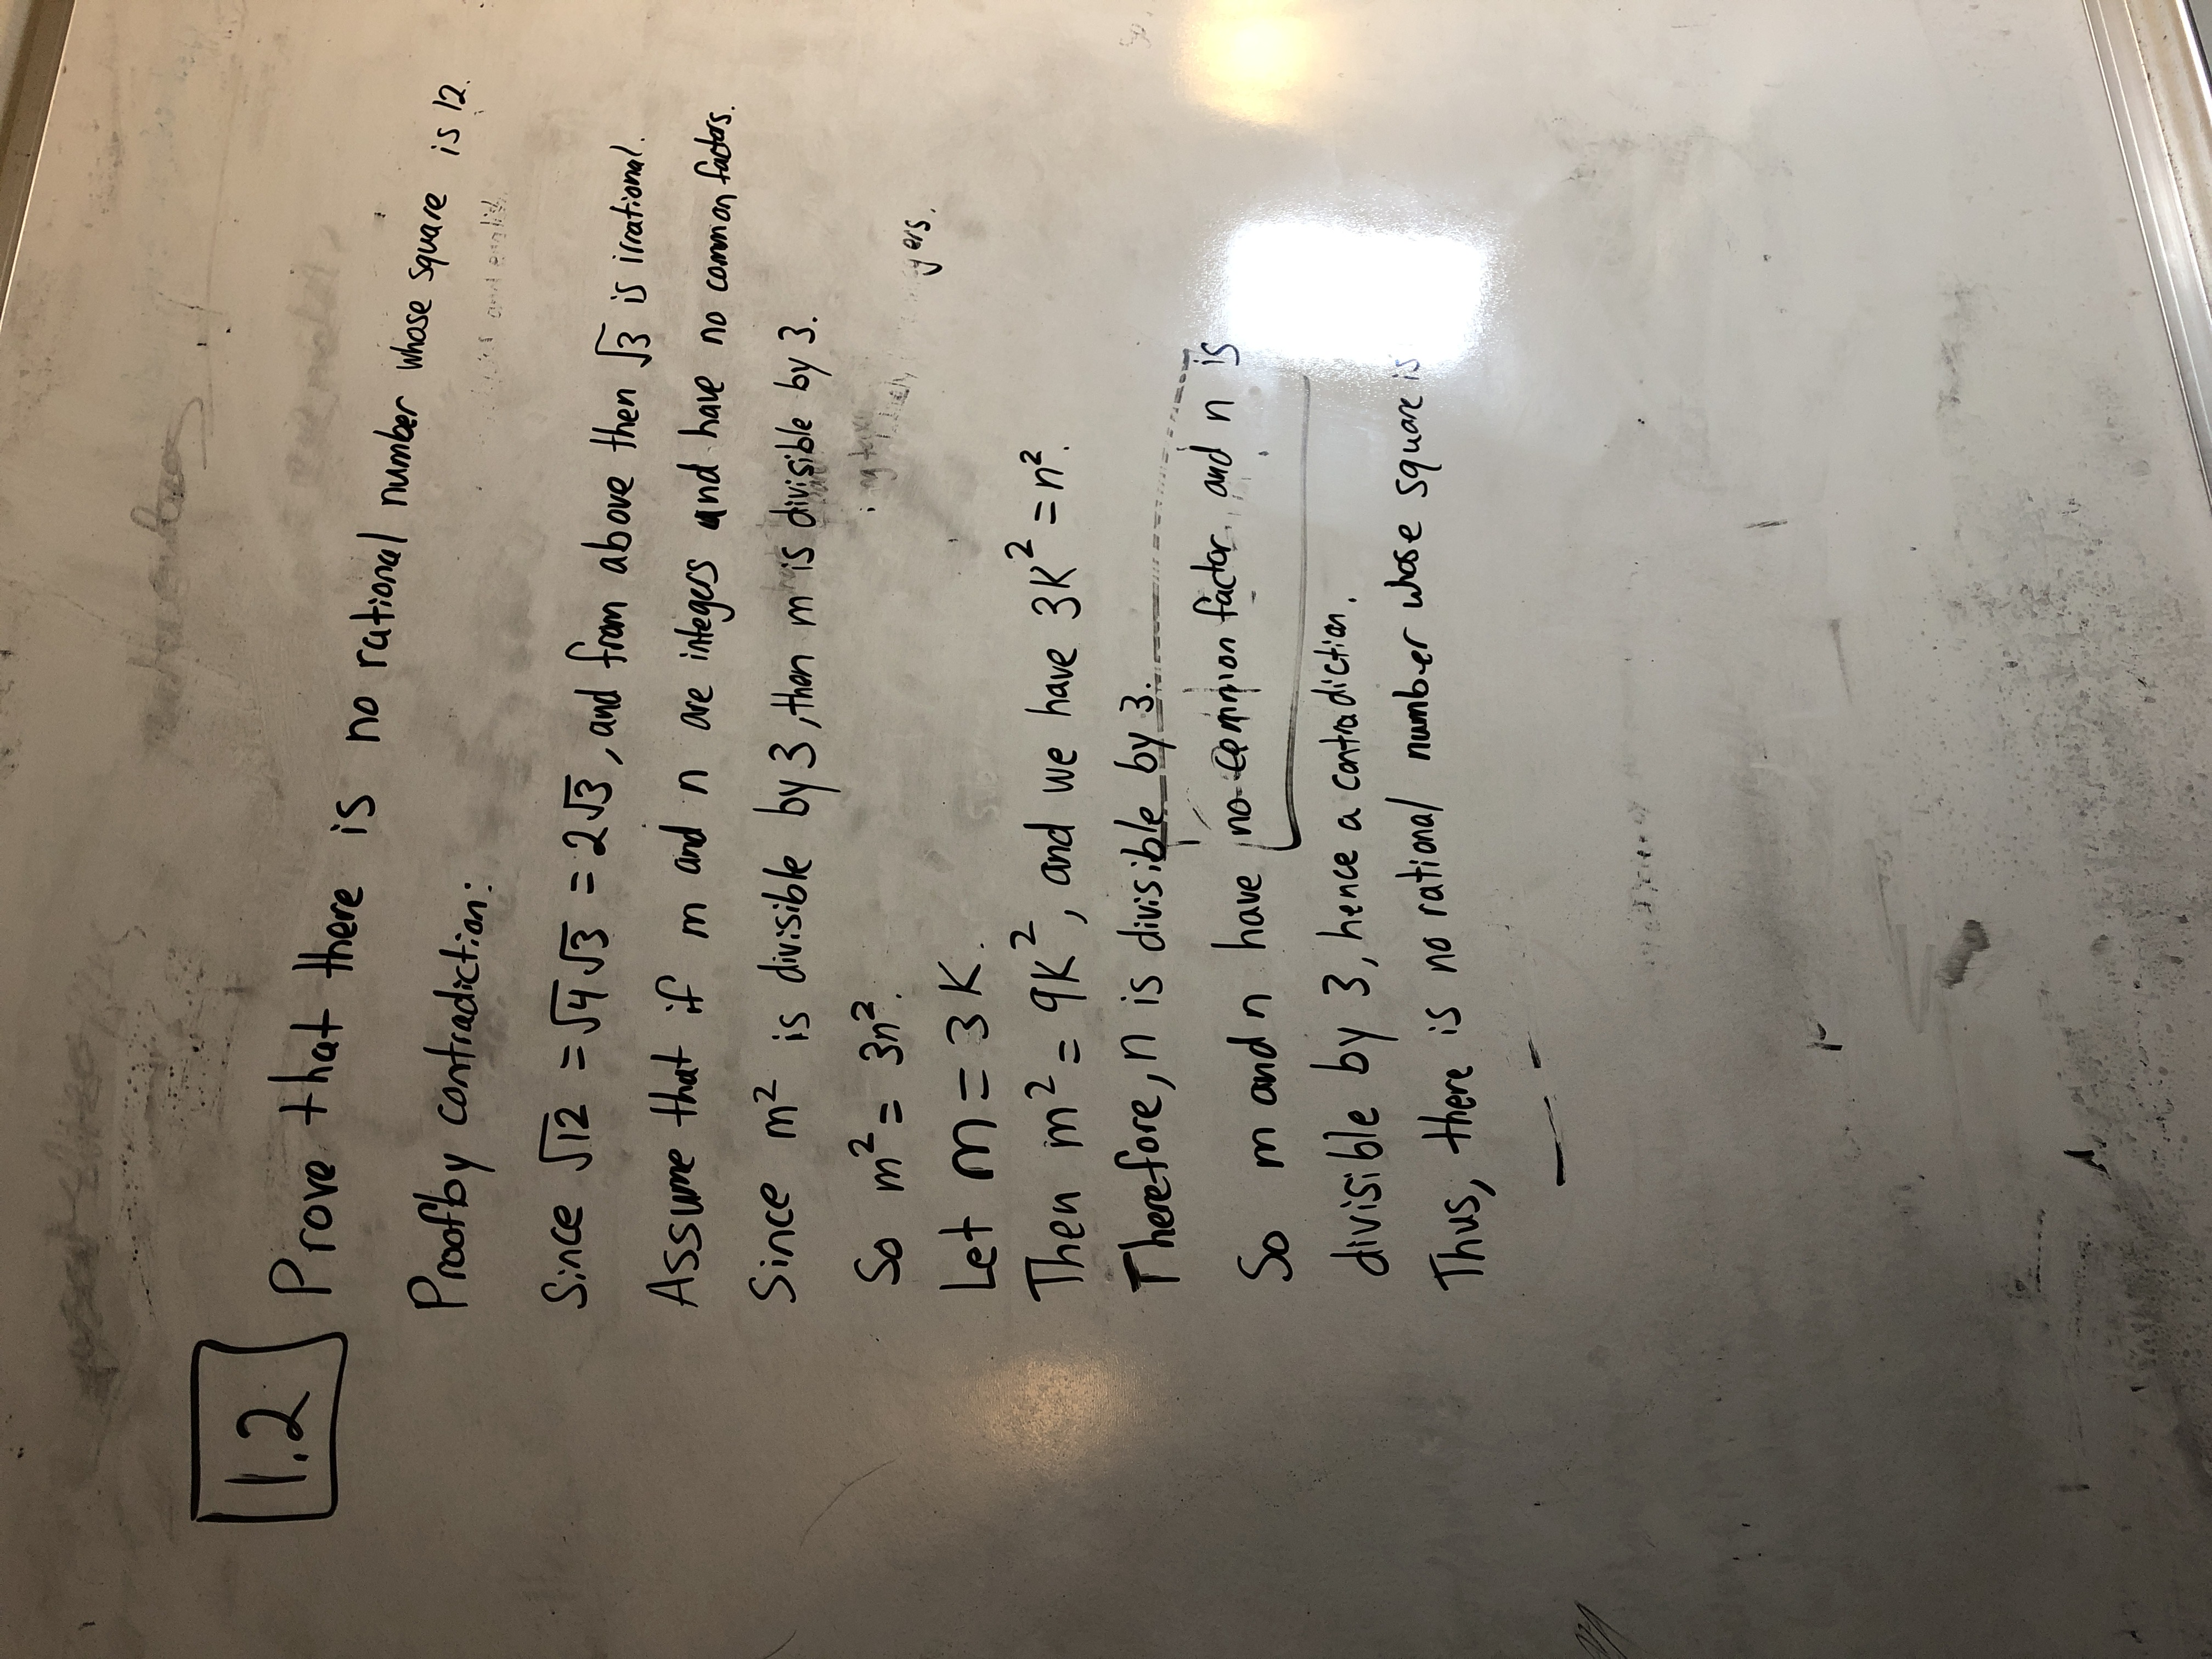
\includegraphics[angle=, origin=c,width=5 in]{Figures/IMG_1077.JPG}
\caption{Placeholder for my proofs} \label{fig:Euler_pic}\end{center}\end{figure} 
\subsection*{Problem 2.3}
Prove that there exist real numbers which are not algebraic. \\ 
\\
Proof:\\ 
As proved above in Problem 2.2, the set of algebraic numbers in the the set of the Real numbers is countable. \\ 
If every real number is algebraic, then the whole set of the real numbers is countable. \\
This is a contradiction, due to "the binary representation of the real numbers (base 2 instead of 10) will notice that Theorem 2.14 implies that the set of all real numbers in uncountable." \\
Thus, there exist real numbers which are not algebraic. 
\begin{figure}[ht]\begin{center}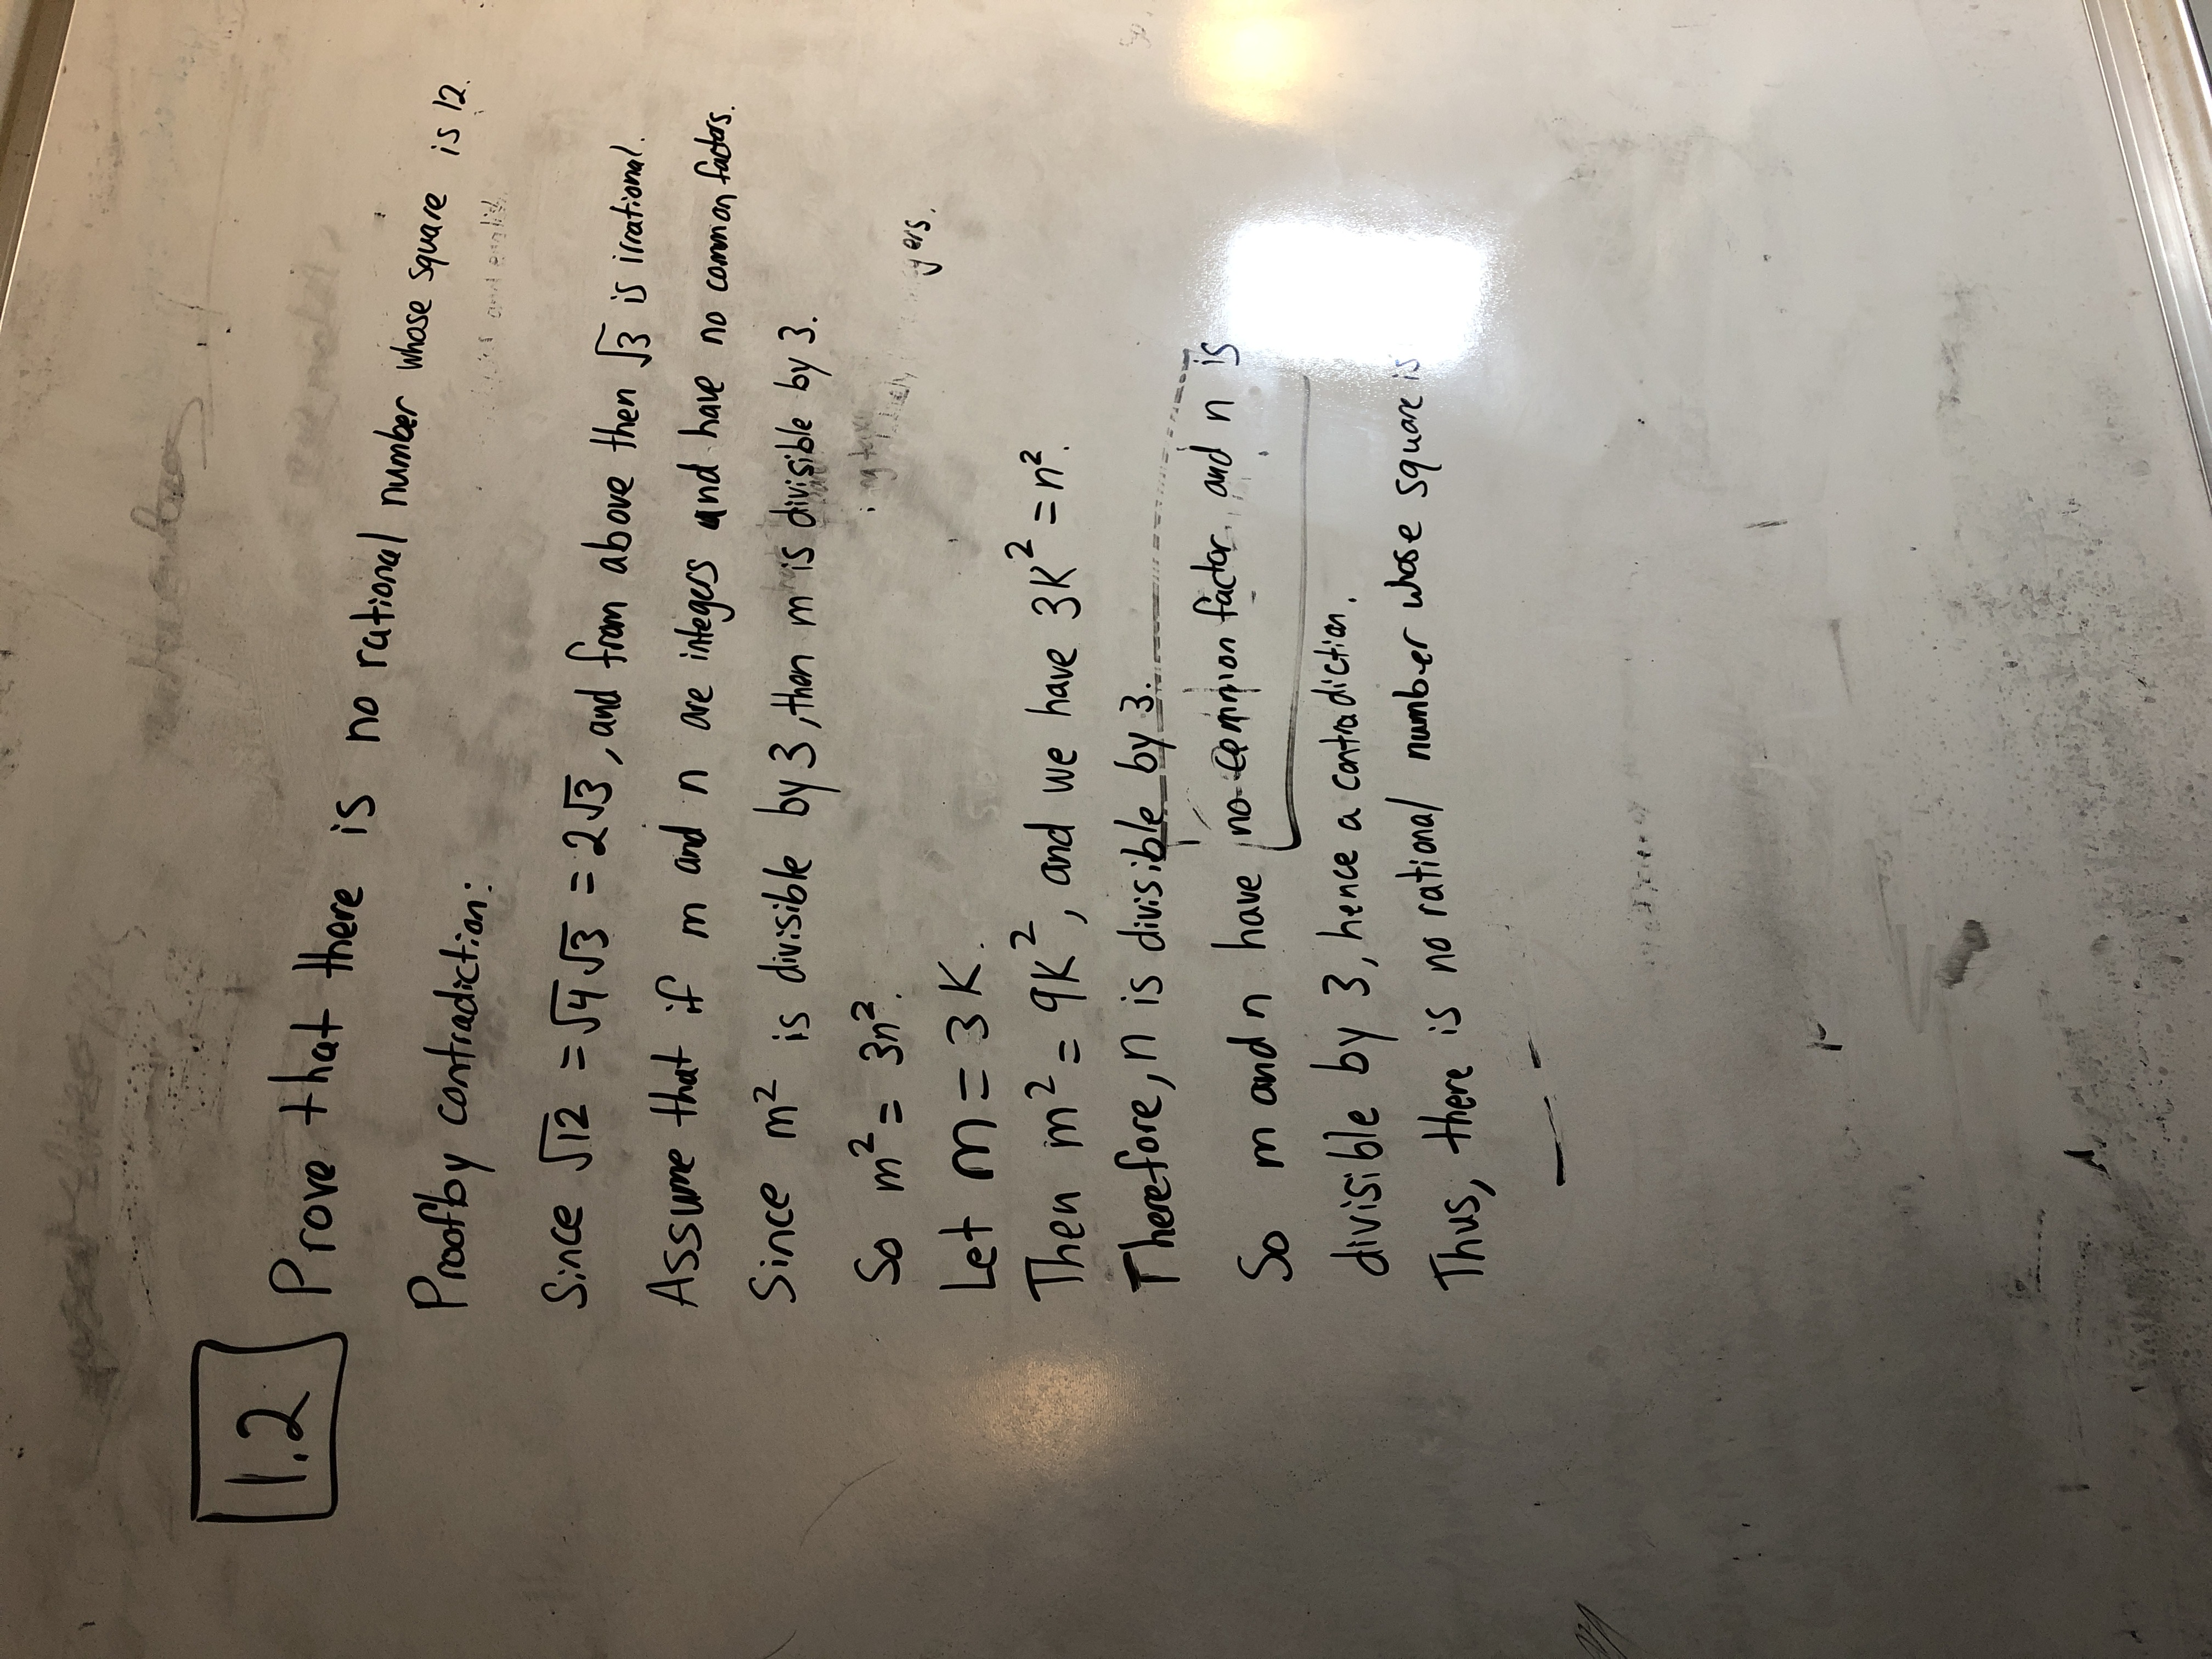
\includegraphics[angle=, origin=c,width=5 in]{Figures/IMG_1077.JPG}
\caption{Placeholder for my proofs} \label{fig:Euler_pic}\end{center}\end{figure} 
\\
\newpage
\subsection*{Problem 2.4}
Is the set of irrational real numbers countable? \\ 
No\\ 
Proof:\\ 
Since the set of real numbers, which is the union of the rational and irrational numbers, is not countable. \\ 
Thus, the set of real irrational numbers is not countable. 
\begin{figure}[ht]\begin{center}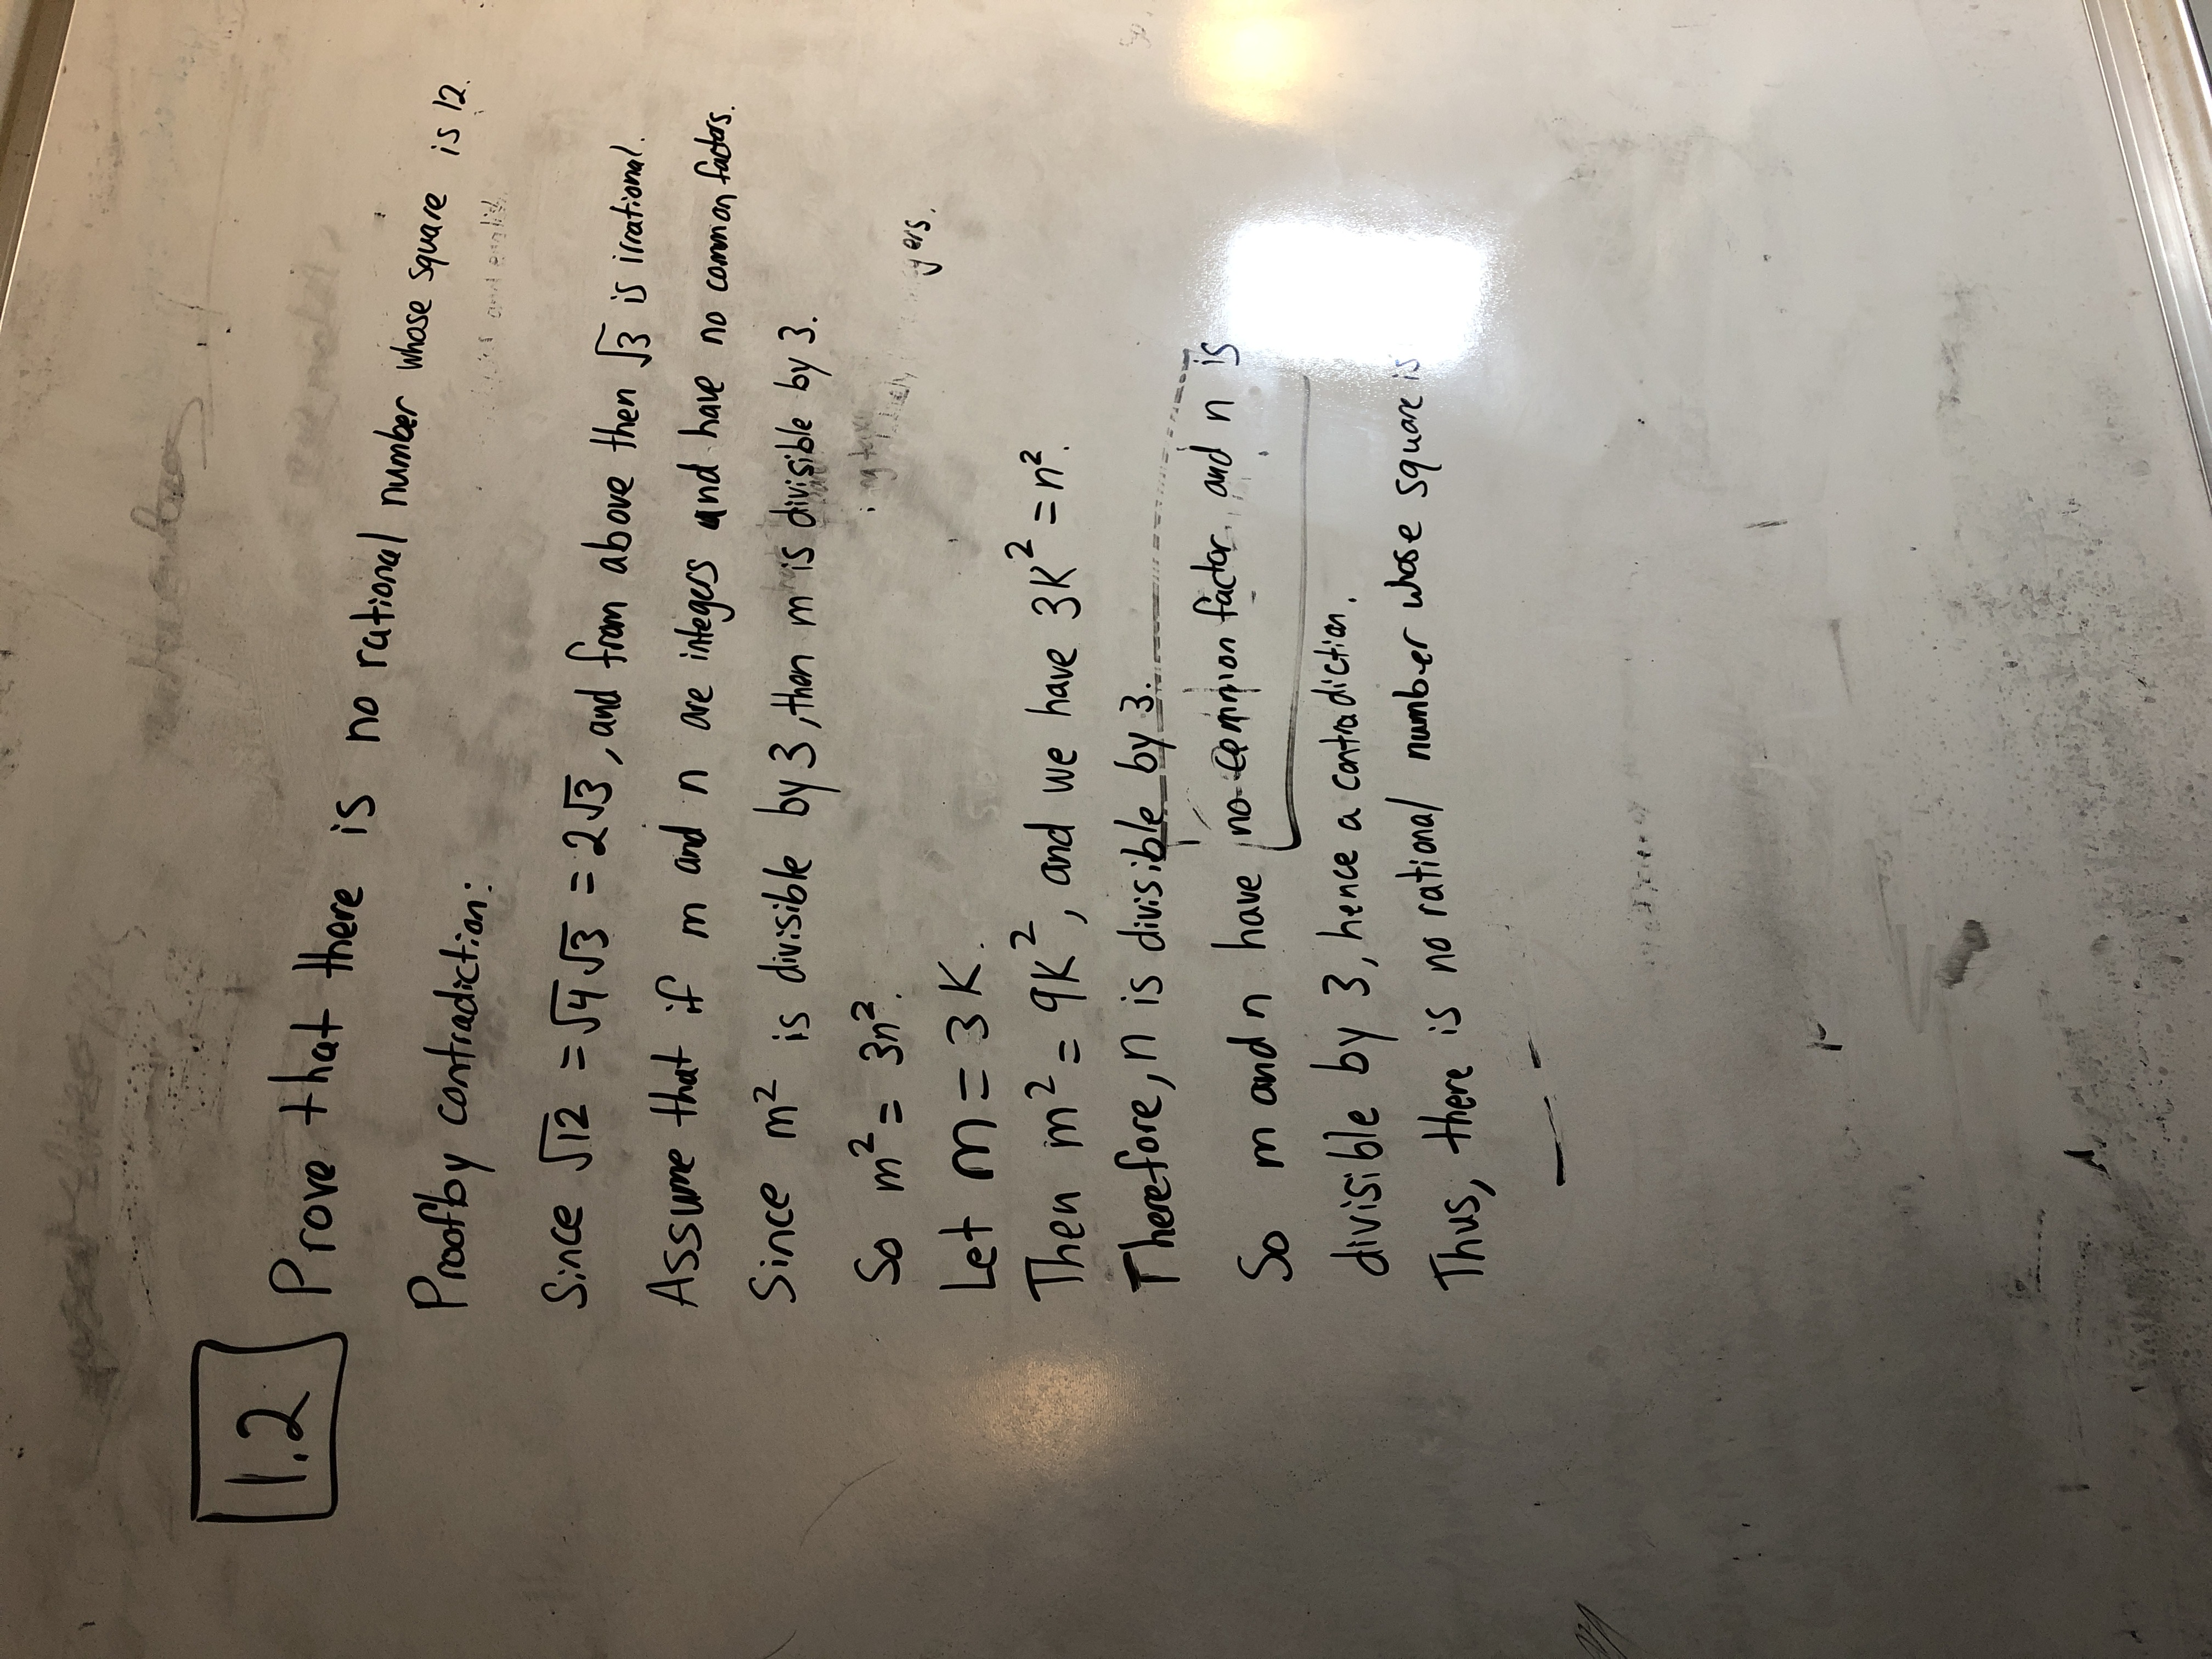
\includegraphics[angle=, origin=c,width=5 in]{Figures/IMG_1077.JPG}
\caption{Placeholder for my proofs} \label{fig:Euler_pic}\end{center}\end{figure} 
\\
\newpage 
\section{Problem 2.5}
Construct a bounded set of real numbers with exactly three limit points. \\
Proof:\\ 
Let E be the set of numbers in $a+ \frac{1}{n},$ where $a \in \{1,2,3\}$ and $n \in \{2,3,4,5, \dots\}.$\\
So, $\{1,2,3\} \subset E^'$, as every deleted neighborhood of 1,2, or 3 contains a point in E.\\
 Let $\delta =$ min ${|x-1|,|x-2|,|x-3|}.$\\
 If $x \notin \{1,2,3\}$, then the set U of y such that $|x-y|< \frac{\delta}{2}$ contains at most a finite number of points of E, since the set $V=(1,1+\frac{\delta}{2}) \cup (2,2+\frac{\delta}{2} \cup (3,3+\frac{\delta}{2})$ is disjoint from U, and V contains all the points of the set E except possibly the finite set of points $a + \frac{1}{n}$ for which $n \leq \frac{2}{\delta}.$ \\
 If $p_1, \dots, p_r$ are the points of E in U, let $N$ be the minimum of $\frac{\delta}{2}$ and the $|x-p_n|$ for which $x \neq p_n.$ \\
 Then the set W of points y such that $|y-x|< N$ contains no points of E except possibly x. \\
 Hence $x \in E^'.$ \\
 Thus $E^{'}=\{1,2,3\}.$


\begin{figure}[ht]\begin{center}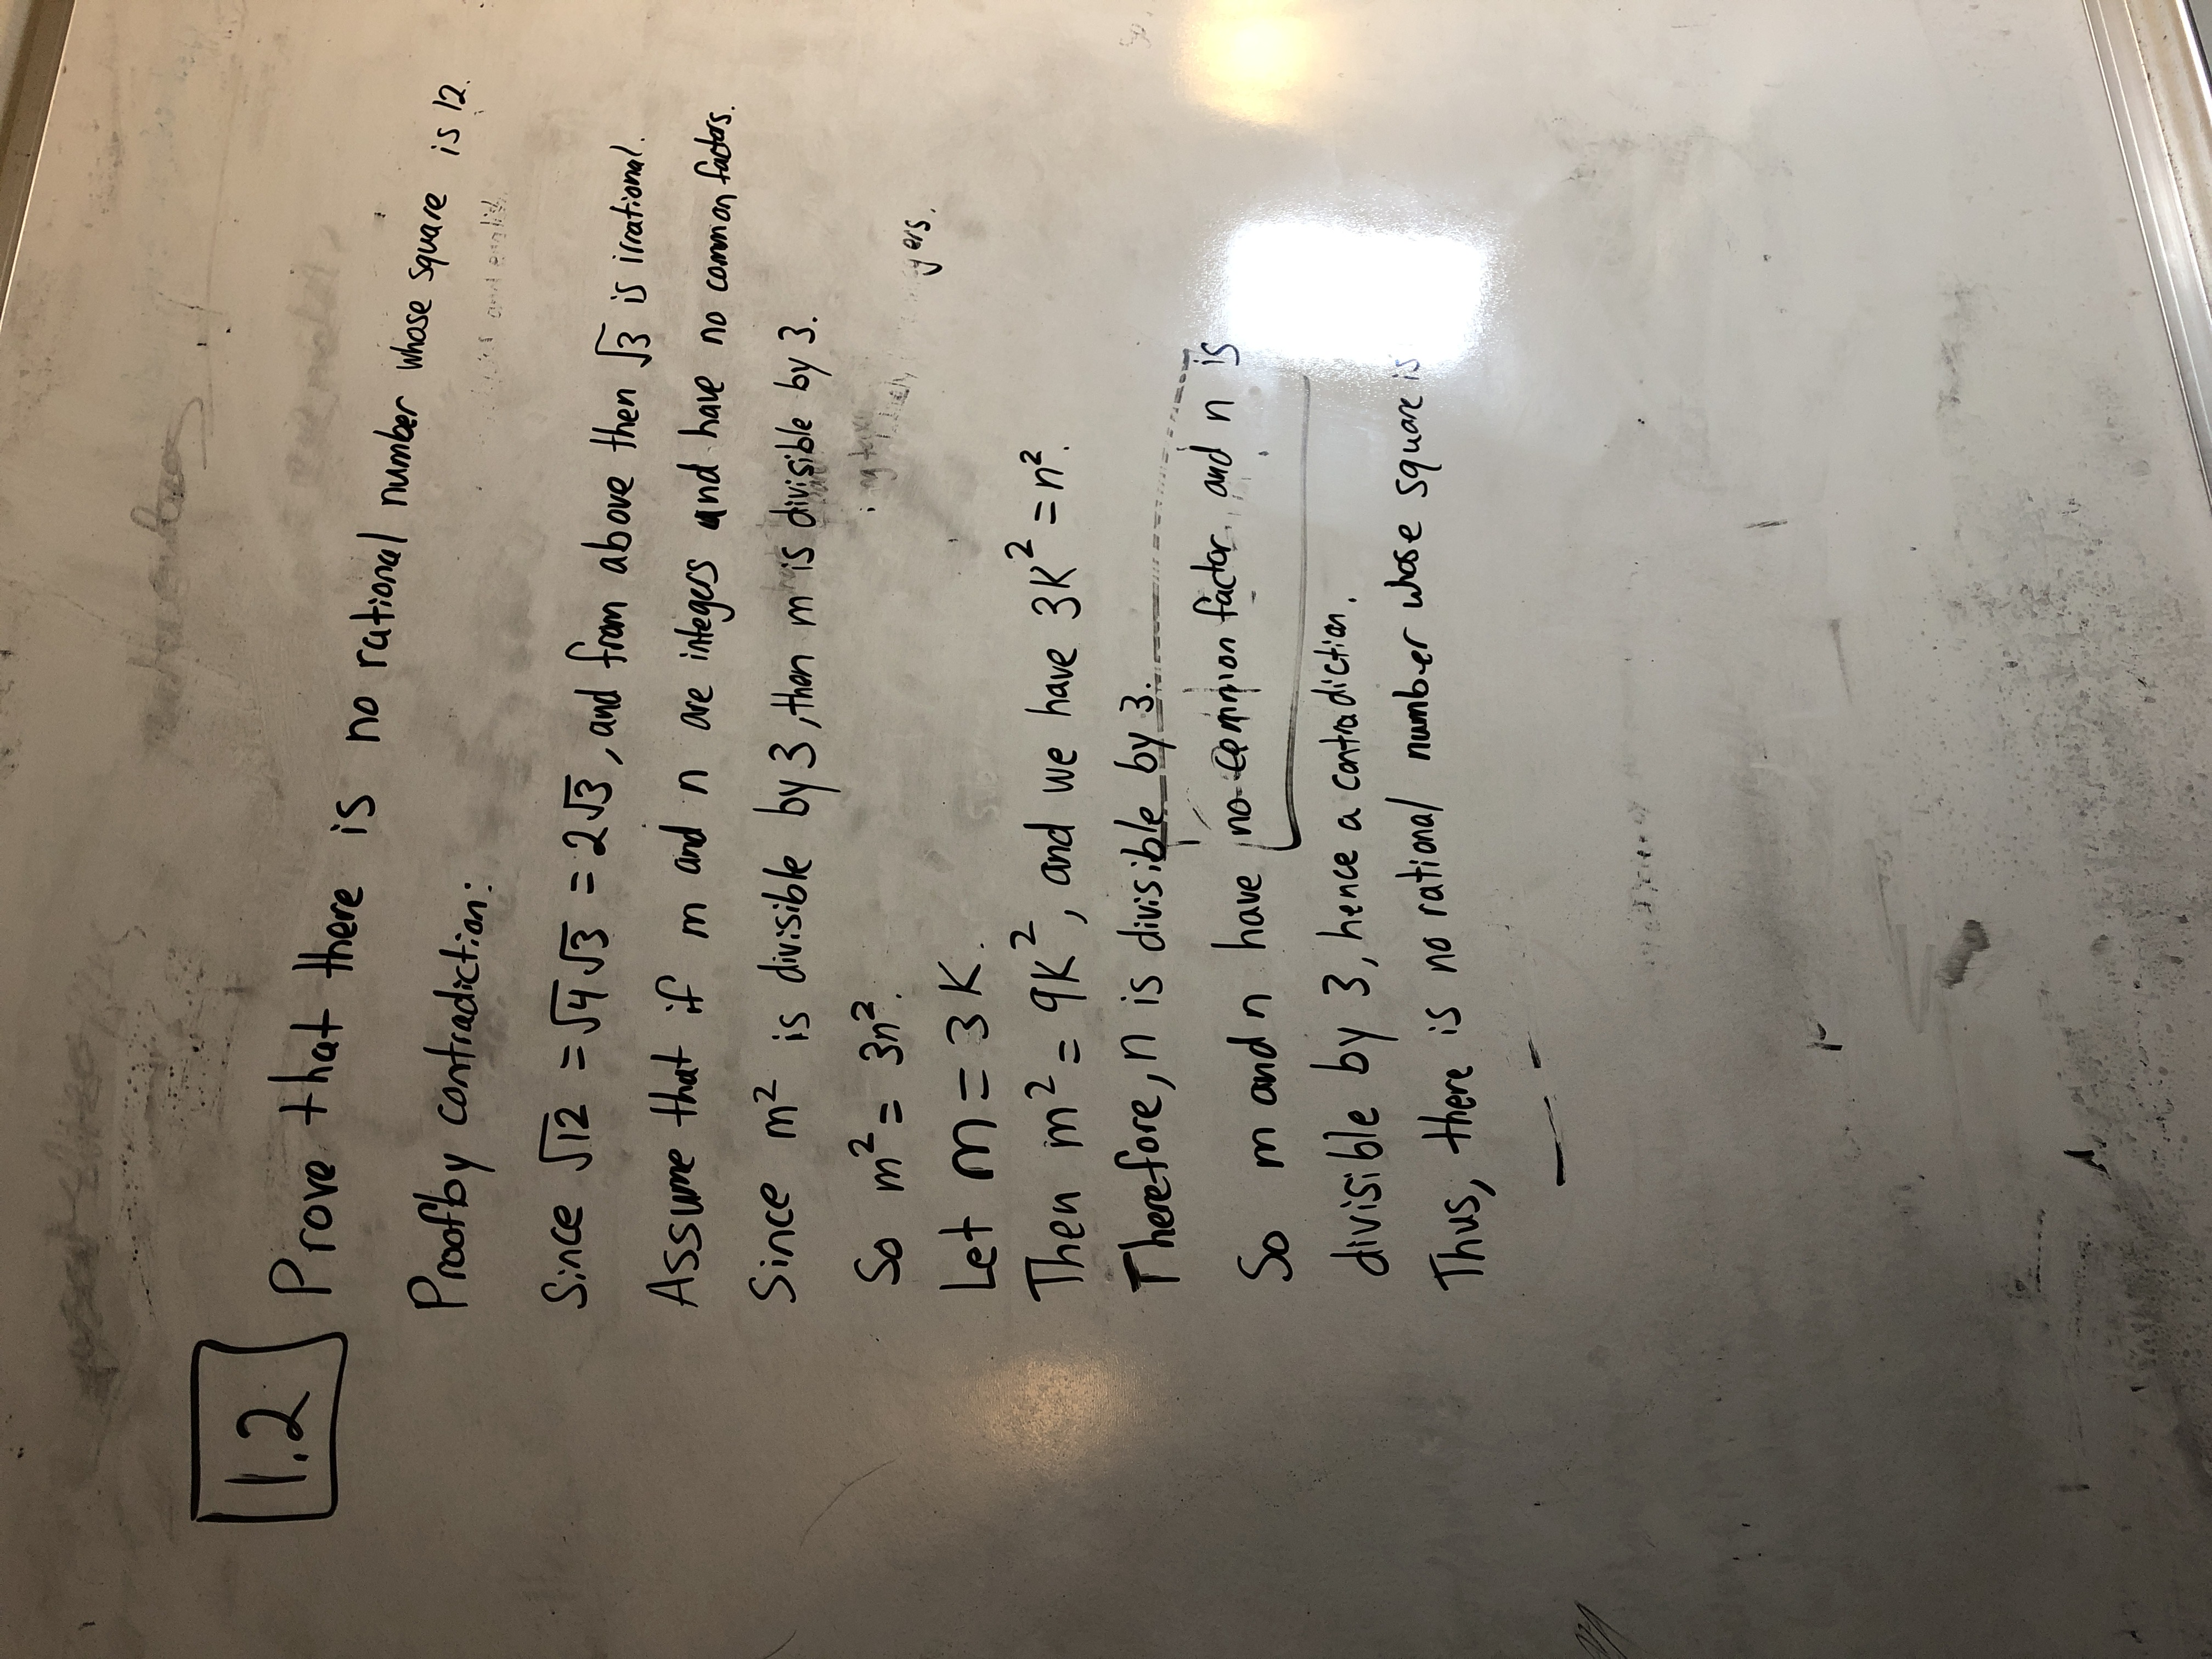
\includegraphics[angle=, origin=c,width=5 in]{Figures/IMG_1077.JPG}
\caption{Placeholder for my proofs} \label{fig:Euler_pic}\end{center}\end{figure} 
\\
\section{Problem 2.6}
Let $E^'$ be the set of all limit points of a set E. Prove that $E^'$ is closed. Prove that E and $\bar{E}$ have the same limit points. (Recall that $\bar{E}=E \union E^'.$) Do E and $E^'$ always have the same limit points?\\ 
Proof:\\ 
Let $x \in (\bar{E})^'.$ \\ 
Let $r>0.$\\ 
There is a point y of $\bar{E}$ such that $0<d(y,x)<r.$ \\ 
If $y \in E^',$ then z=y. \\ 
If $y \notin E$, then $y \in E^'.$ \\ 
Let $s=min(d(x,y)),r-d(x,y)),$ where $s>0.$ \\ 
Since $y \in E^',$ there exists $z \in E$ with $0<d(x,z)<s.$ \\ 
So $d(z,x) \geq d(x,y)-d(x,z)>0$ and $d(z,x) \leq d(x,y)+d(y,z)<d(x,y)+r -d(x,y)=r.$ \\ 
Next, demonstrate that E and $\bar{E}$ have the same limit points. \\ 
Suppose $x \in E^'.$ \\ 
Since every deleted neighborhood of x contains a point of E, then furthermore every deleted neighborhood of x contains a point of $\bar{E}.$ \\ 
Thus, $E^{'} \subseteq (\bar{E})^'.$ \\ 
So, E and $E^'$ may have different sets of limit points. \\ 
So one case would be if $E=\{0,1,\frac{1}{2},\frac{1}{3}, \dots, \frac{1}{n}, \dots\},$ then $E^{'}={0},$ while $(E^{'})^{'}= \emptyset.$

\begin{figure}[ht]\begin{center}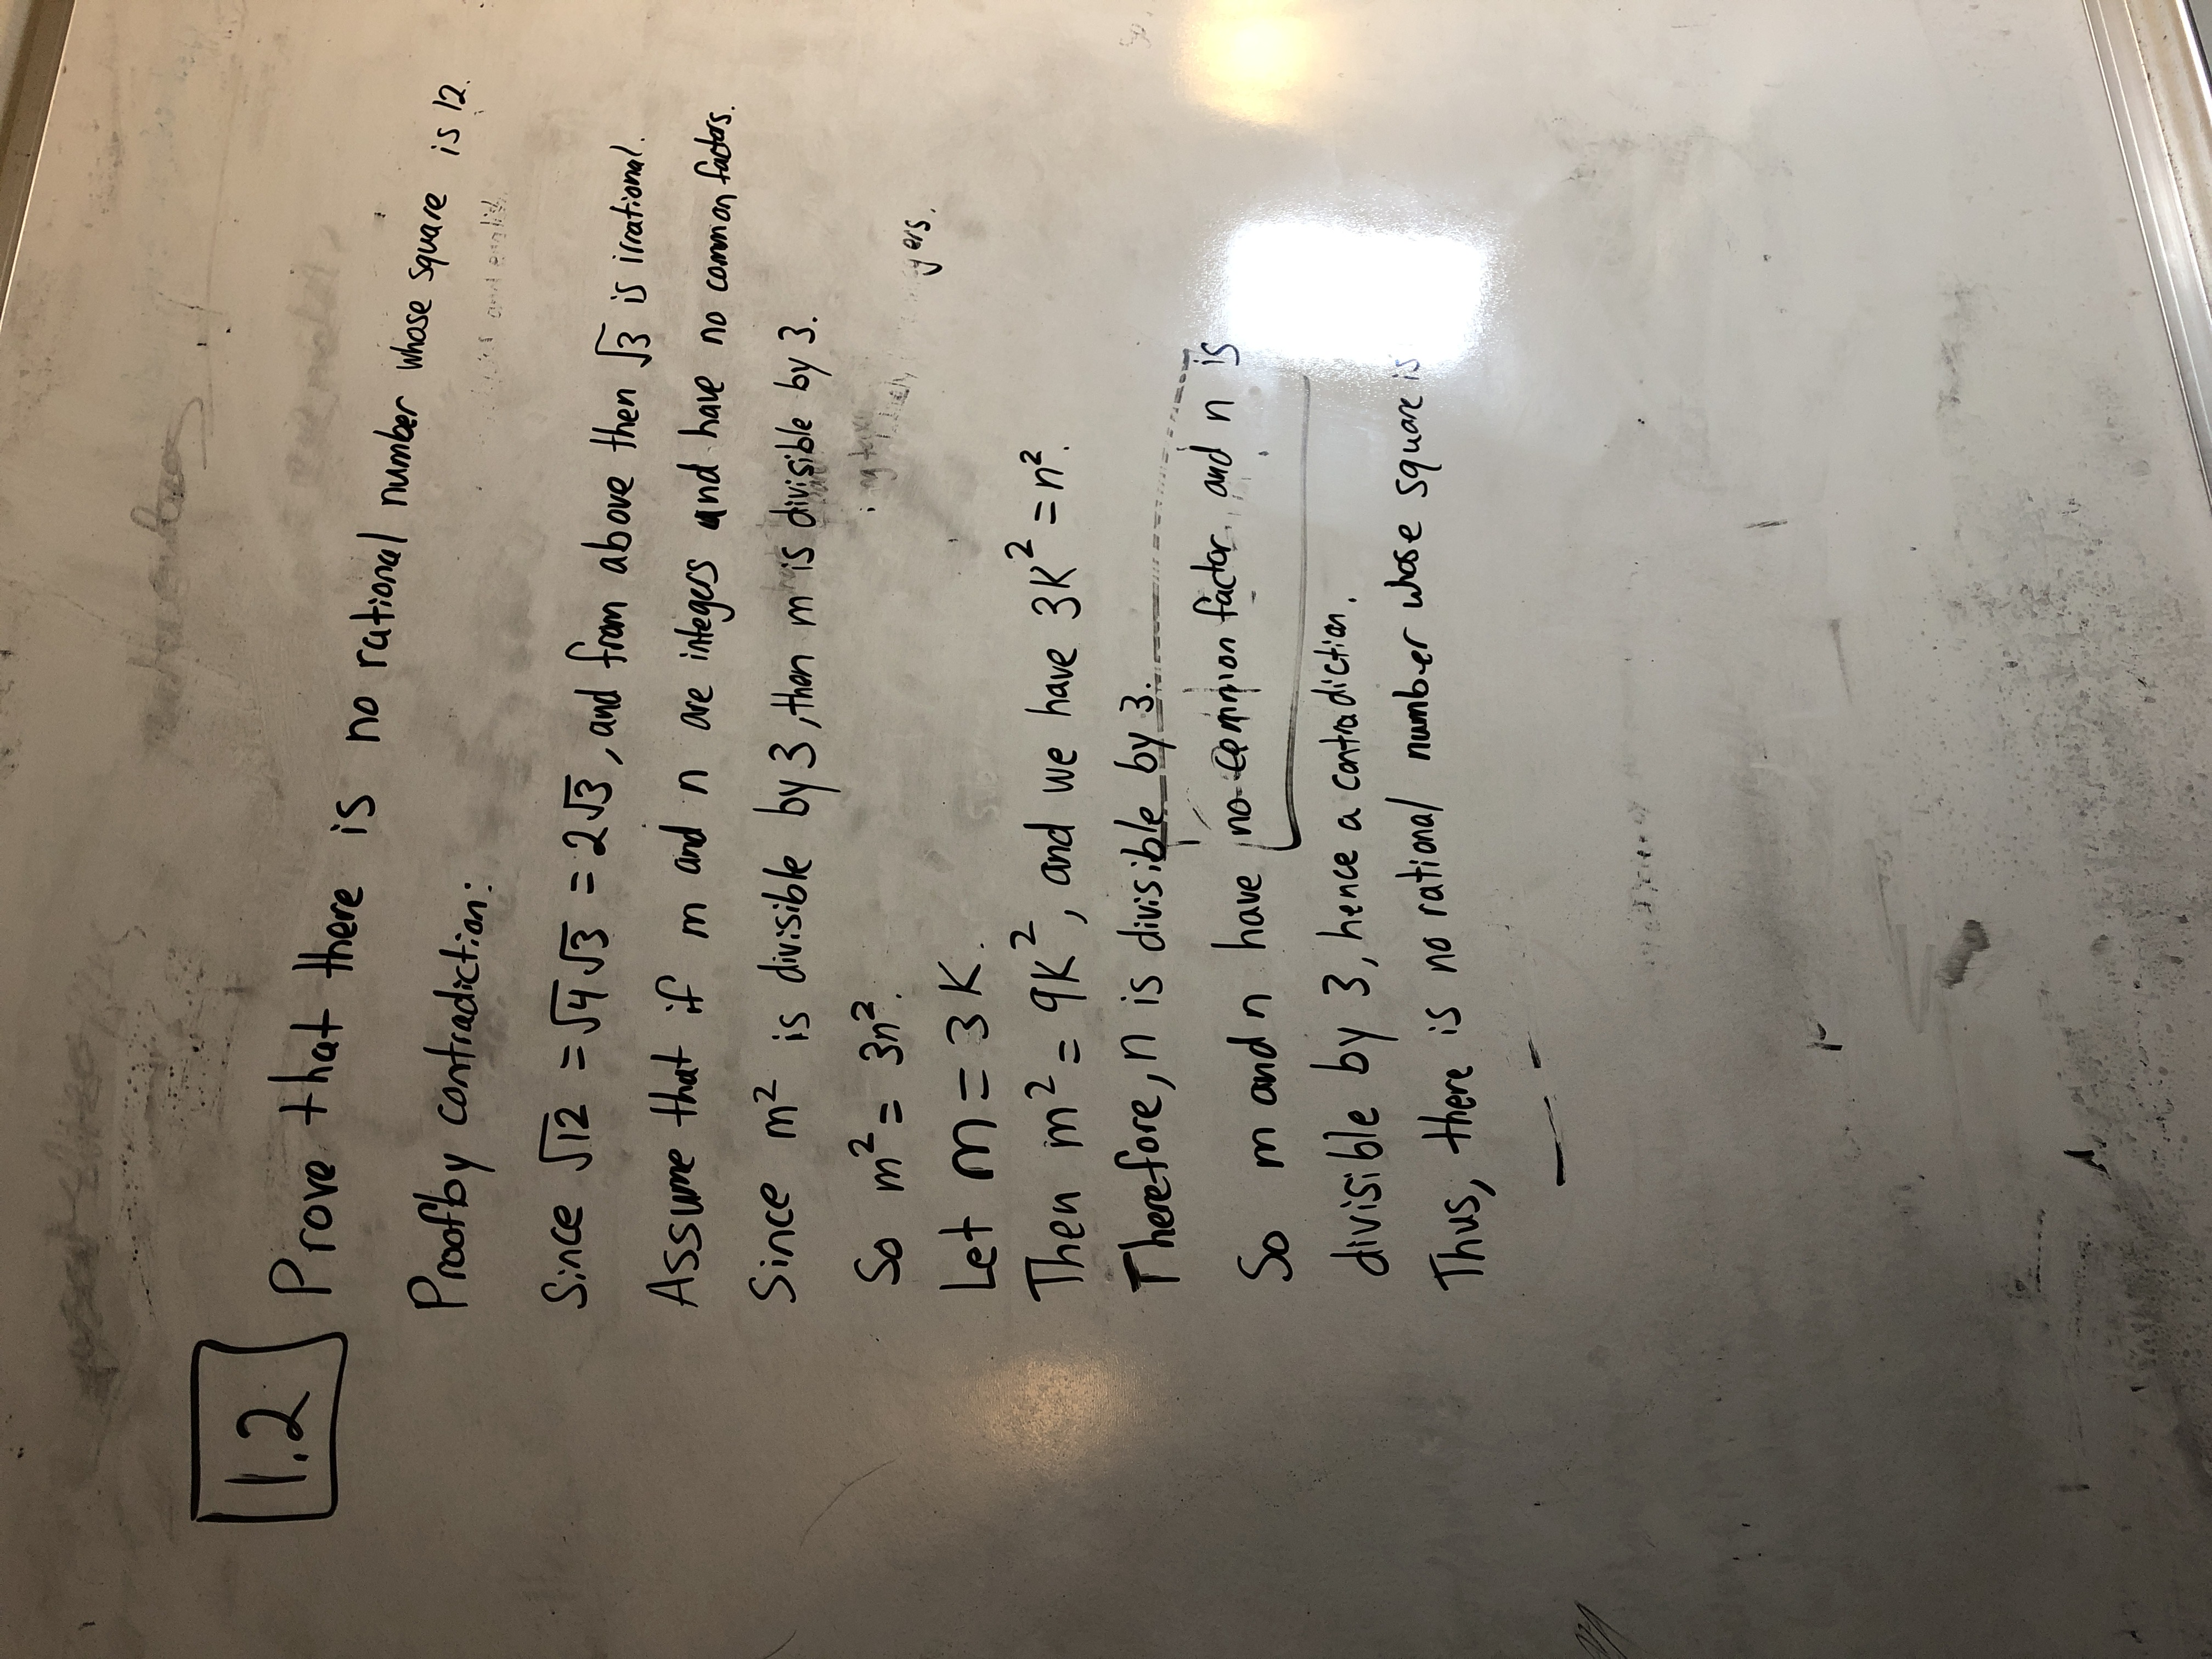
\includegraphics[angle=, origin=c,width=5 in]{Figures/IMG_1077.JPG}
\caption{Placeholder for my proofs} \label{fig:Euler_pic}\end{center}\end{figure} 












\newpage

\section{The First Compilation}

\section*{Me Pontificating}

\section*{Questions to pay attention to and ask Dr. Ross about This is Due by Monday}
\section*{What to talk to Dr. O'Shaugnessy about}
Random walks and what not 
\section*{Finite, Countable, Uncountable Sets}
For each of the following sets, determine whether the set is finite, countable, or uncountable. Prove your claims. \\
\subsection*{The real numbers that can be expressed as infinite sums}

\subsection*{The set of all possible Soduku Puzzles}


\subsection*{The real numbers that can be expressed as infinite sums something something binary numbers}


\subsection*{All of the pages in all of the books that have ever been printed}

\subsection{Natural Numbers one}
The set of all functions whose domain is $\N$ and whose range is the finite set $\{0,1,2,3,4,5,6,7,8,9\}$

\subsection*{The set consisting of all binomial coefficients}

\section*{Inner Product and Dot Product just think about the tensor product and this hell will be over soon}\\ 
\textbf{In other news why I should care about this other than for my gpa and to continue my research and be off of probation due to my stress associated with my family during a pandemic...photons and how the dot product is 0 since they are massless particles the dot product as relates to the general relativity minkowski metric }\\
In $R^k$consider the inner product- an inner product that is not the usual dot product-that is defined, for vectors $\Vec{x}=(x_1,x_2,...,x_k)$ and $\Vec{y}=(y_1,y_2, ..., y_k)$ by the formula \\ 
$\Vec{x} * \Vec{Y}= \Sigma_{j=1}^{k}c_j x_j y_j$ \\ 
where $c_1, c_2, ... c_k$ are positive real numbers. We define a vector norm, $||\Vec{x}||_{*}=\sqrt{\Vec{x}*\Vec{x}}$ and we define a function $d_*(\Vec{x}, \Vec{y})=||\Vec{x}-\Vec{y}||_*=\sqrt{(\Vec{x}-\Vec{y}*(\Vec{x}-\Vec{y})}$ \\ 
Now we have two different inner products, the one we just introduced, $\Vec{x}*\Vec{y}=\Sigma_{j=1}^k c_{j}x_{j}y_{j}$ with its associated norm, $||\Vec{x}||_*=\sqrt{\Vec{x}*\Vec{x}}$ and the metric, $d_{*}(\Vec{x},\Vec{y})=||\Vec{x}-\Vec{y}||_{*}=\sqrt{(\Vec{x}-\Vec{y})*(\Vec{x}-\Vec{y})}$ and the standard inner product, $\Vec{x}\dot\Vec{y}=\Sigma_{j=1}^{k}x_jy_j$ with its associated norm $||\Vec{x}||_2 = \sqrt{\Vec{x}\dot \Vec{x}}$ and the metric $|\Vec{x}-\Vec{y}|=\sqrt{(\Vec{x}-\Vec{y}\dot \Vec{x}-\Vec{y})}$ \\ 



\section{Finite, countable, or uncountable sets}
For each of the following sets, determine whether the set is finite, countable, or uncountable. Prove your claims. \\ 
\subsection{Infinite sums}
The real numbers that can be expressed as infinite sums of the form $x= \sum_{j=k}^\infty q^{j}$ where k is a nonnegative integer and q is a rational number. 
\\ 
It is countable.
\subsection{Sudoku}
The set of all possible Sudoku puzzles.
\\ 
It is countable. The number of different puzzles would be a large number for all the different permutations, but it would be finite and countable. \\ 


\subsection{Another infinite sum} 
The real numbers that can be expressed as infinite sums of the form \\ 
$x= \sum_{j=0}^\infity b_j2^{-j}$ where each $b_j$ is either 0 or 1. \\ 

This would be uncountable. 
\subsection{Book Pages}
All of the pages in all books that have ever been printed. 
\\ 
It is a growing number. It is countable since it could be feasible to calculate this number, but it is not realistic since books may have been burned so since the word ever is used it may not be that way. 

\subsection{Domain and range}
The set of all functions whose domain is the Natural numbers and whose range is the finite set ${0,1,2,3,4,5,6,7,8,9}.$
This would be uncountable. 
\subsection{Binomial Coefficients}
The set consisting of all binomial coefficients.
\\ 
This would be countable since the permutation would be the natural numbers cross the natural numbers. 
\section{Inner Product}
In $R^k$ consider the inner product- an inner product that is not the usual dot product-that is defined, for vectors $\vec{x}=(x_1, x_2,..., x_k)$ and $\vec{y}=(y_1,y_2,...,y_k)$ by the formula \\ 
$\vec{x}*\vec{y}= \sum_{j=1}^k c_j x_j y_j$ \\ where $c_1,c_2,...,c_k$ are positive real numbers. We define a vector norm, $||\vec{x}||_{*}=\sqrt{\vec{x}*\vec{x}}$ and we define a function $d_*(\vec{x},\vec{y})=||\vec{x}-\vec{y}||_{*}=\sqrt{(\vec{x}-\vec{y}*(\vec{x}-\vec{y}}.$\\ 
Now we have two different products, the one we just introduced, $\vec{x}*\vec{y}= \sum_{j=1}^k c_j x_j y_j$, with its associated norm, $||\vec{x}||_{*}=\sqrt{\vec{x}*\vec{x}}$ and the metric, $d_*(\vec{x},\vec{y})=||\vec{x}-\vec{y}||_{*}=\sqrt{(\vec{x}-\vec{y}*(\vec{x}-\vec{y}}$ and the standard inner product, $\vec{x}\cdot \vec{y}= \sum_{j=1}^k x_j y_j$ with its associated norm $||\vec{x}||_{2}=\sqrt{\vec{x}\cdot \vec{x}}$ and the metric $\vec{x}-\vec{y}=\sqrt{(\vec{x}-\vec{y})\cdot (\vec{x}-\vec{y})}$. \\ 
\subsection{Schwartz Inequality}
State and prove the analog of the Schwartz inequality for $\vec{x}*\vec{y}.$ \\ 
Theorem 1.35. \\ 
If $a_1,...,a_n$ and $b_1,...,b_n$ are complex numbers then $|\sum_{j=1}^n a_j \bar{b_j}|^2 \leq \sum_{j=1}^n |a_j|^2 \sum_{j=1}^n |b_j|^2.$ \\ 

\subsection{Positive real numbers M} 
Prove that there are positive real numbers M and m such that for all vectors $\vec{x}$ and $\vec{y}$ \\ 
$|\vec{x}\cdot \vec{y}\leq M ||\vec{x||_{*}}||\vec{y||_{*}}$ and \\ $m|\vec{x}*\vec{y}\leq ||\vec{x}||_2||\vec{y}||_2$ and find the largest such m and the smallest such M. \\ 
\subsection{c_j = j} 
For k=5, consider the case in which $c_j=j.$ For an arbitrary $\vec{x}=(x_1,x_2,...,x_k),$ find a non-zero $\vec{y}=(y_1,y_2,...,y_k)$ such that $\vec{x}*\vec{y}=0.$ \\ 
\subsection{If c was not positive} 
If not all $c_1,c_2, ...,c_k$ were positive, $d_{*}(\vec{x}, \vec{y})$ would no longer be a metric. Why? 
\section{Metric Space}
Let X be a metric space. A subset A is said to be dense in X if $\bar{A}=X,$ that is, if the closure of A is X. Prove that the following statements are equivalent; that is, prove that if any one of them is true they are all true:\\ 
The set A is dense in X. \\ 
The only closed set that contains A is X. \\ 
There is no non-empty open set that is disjoint from A. \\ 
The set A intersects every neighborhood. \\ 
\section{Definition 2.45 Rudin}
Two subsets A and B of a metric space X are said to be separated if $A \cap \bar{B}$ and $B \cap \bar{A}$ are both empty, that is, if A is disjoint from the closure of B and B is disjoint from the closure of A. A set E in X is said to be connected if it is not the union of two non-empty separated sets. This is just Definition 2.45 in Rudin. \\ 
\subsection{Convex Set}
Prove that every convex set in $R^k$ is connected. \\ 
Definition 2.17 \\ 
We call a set $E \subset R^k$ convex if $\lambda x + (1- \lambda) y \in E$ whenever $x \in E,$ $y \in E,$ and $ 0< \lambda <1.$
\subsection{Two Subsets are separated}
Consider this claim: Two subsets A and B of a metric space X are separated if and only if $\bar{A} \cap \bar{B}$ is empty. If it's true, prove that it's true; if it's false, prove that it's false. \\ 
\section{Uncountable Collection}
Give an example of an uncountable collection of disjoint closed sets in $R^2$ \\ 
$\cup_{x \in R^2} x$
\section{Prove that there is a finite collection}
Let K be a compact subset of a metric space X. Suppose that $F_{\beta}$ is a collection of closed sets contained in K and that $\cap_{\beta} F_{\beta}$ is empty. Prove that there is a finite collection of these closed sets with an empty intersection. 



\section{Chapter 2 Baby Rudin}

\section{The Second Compilation}
\section*{Me Pontificating}
Here is me being a control freak and doing all the work now so I can return to my simulations and practice numerical relativity projects with CCRG as planned. Thank you for your understanding. I do need an A in this course as the fellowships, scholarships, grants, programs, and institutions I am interested in do indeed care about my final gpa. Please provide any feedback for these cases. \\ 

\section*{Dr.O'Shaugnessy why is it cool and relates to my research?: Independent Study and engagement idea to have me not go rogue and research and study optics and fourier analysis and tensors and question why I'm classified as a math major at this institution}

\section{Cesaro Summable Question }

\subsection{The Problem itself}


\subsection{Relevant readings}

\subsection{Me pontificating}


\subsection{Proofs and work}


\section{Newton's method}

\subsection{The Problem itself}
(25 pts) Newton's method for estimating the real cube root of a positive real number Z is to start with an arbitrary guess, $x_0,$ and to generate an infinite sequence ${x_n}$ recursively with the recursion relation \\ 
$x_{n+1}=\frac{2}{3}x_{n}+\frac{1}{3}\frac{z}{x_n^2}$\\ 

Prove that if $x_0 >0, $ then as long as none of the iterates equals zero the sequence ${x_n}$ converges to the cube root of Z. There are some negative values of $x_0$ for which the sequence ${x_n}$ does not converge, values for which the recursion formula that defines the sequence produces an undefined term because of a would-be division by 0 after a finite number of terms. Characterize those negative values of $x_0$ and prove that for all other negative values of $x_0$ the sequence ${x_n}$ converges to the cube root of Z.

\subsection{Me pontificating}

\subsection{Proofs and work }


\section{Convergence series}


\subsection{Me Pontificating}
Why would I care? My research is based on Bayesian statistics converging methods. I mean this is the simplistic look at the idea...but the exercise has merit and I should be looking at O3 and O4.  
\subsection{The problem itself}
(25 Points) \\ 
Let $b_n=$ \[ \begin{cases} 
      1 & 2^{2k}\leq n <2^{2k+1} \\
      -1 & 2^{2k+1} \leq n\leq 2^{2k+2} 
   \end{cases}
\] 
for K=0,1,2,... \\ 
Determine whether the series $\sum_{n=2}^\infty \frac{b_n}{n log(n)}$ converges. Prove your claim. (9 points). \\ 
\begin{figure}[h]\begin{center}\includegraphics[angle=, origin=c,width=2 in]{WhiteboardPictures/Exam 2/IMG_1052.JPG}
\caption{Placeholder for my proofs} \label{fig:Euler_pic}\end{center}\end{figure} 

\newpage
Determine whether the series $\sum_{n=2}^\infty \frac{b_n}{n}$ converges. Prove your claim. (8 points). \\ 
\begin{figure}[h]\begin{center}\includegraphics[angle=, origin=c,width=2 in]{WhiteboardPictures/Exam 2/IMG_1052.JPG}
\caption{Placeholder for my proofs} \label{fig:Euler_pic}\end{center}\end{figure} 

\newpage 
Determine whether the series $\sum_{n=2}^\infty \frac{b_n}{n^2}$ converges. Prove your claim. (8 points). \\ 

\begin{figure}[h]\begin{center}\includegraphics[angle=, origin=c,width=2 in]{WhiteboardPictures/Exam 2/IMG_1052.JPG}
\caption{Placeholder for my proofs} \label{fig:Euler_pic}\end{center}\end{figure} 

\newpage


\section{Bifurcation Diagram}


\subsection{Me Pontificating about why I care about chaos dynamics}
This is rudimentary newton's method and the time complexity is baseline. 


\subsection{The Problem Itself}
(25 points total) In a seminal paper May [1] presented and analyzed simple difference equation
models of biological systems that have chaotic dynamics. May and other researchers in this field
emphasize, as a typical example, the logistic model as expressed in this recurrence formula: \\ 
$x_{N+1}=rX_N(1-X_N)$ \\ 
Here, $X_N$ is a population at the Nth time period after the initial time period. (See[1] and particularly [3] for examples). The parameter r is fixed. We start with an initial population— $x_0$
 —
and the formula lets us compute the population at successive time periods. (The Wikipedia article
on this topic [2] is worth reading.) The recurrence formula produces an infinite sequence that
characterizes the evolution of the population; that sequence depends on r and $x_0$
.
For the formulation given by our recurrence relation, r is positive and 0 < $x_0$ < 1.
This model is associated with an interesting and famous bifurcation diagram: \\ 


You should read the Wikipedia article [2] for a thorough account of this diagram; I am just going to
summarize the bits that are important for this problem. For values of r between 2 and 3, the
sequence produced by the recurrence formula converges, and for a fixed r all of the sequences,
regardless of $x_0$
 , converge to the same value. This is why there is a single point on each line r = constant between 2 and 3 on the bifurcation diagram. For values of r between 3 and about 3.45,
the sequence produced by the recurrence formula does not converge, but asymptotically its
elements oscillate between two values, and for a fixed r all of the sequences—with one
exception--regardless of $x_0$
 , oscillate asymptotically between the two values. This is why there
are two points on each line r = constant between 3 and about 3.45, on the bifurcation diagram.
For values of r between about 3.45 and about 3.54, the sequence produced by the recurrence
formula does not converge, but asymptotically its elements oscillate among four values, and for a
fixed r all of the sequences—with a few exceptions--regardless of $x_0$
 , oscillate asymptotically
among the four values. This is why there are four points on each line r = constant between about
3.45 and about 3.54, on the bifurcation diagram.
Prove that if 0 < r < 1 all of the sequences produced by the recurrence formula converge—that
is, for all values of $x_0$
 between 0 and 1---to 0. (5 points)
Prove that for any fixed r such that 1 < r < $2 \sqrt{2}$ all of the sequences produced by the
recurrence formula converge—that is, for all values of $x_0$
 between 0 and 1---to the same number. \\ 
 (10 points) Here are some hints (but you needn’t follow them, prove the result in any way you’d
like to):
 Show, from the recurrence relation $x_{N+1}=rX_N (1-X_N)$ that for all values in the specified
ranges of r and $x_0$
 , $0<X_N \leq \frac{r}{4}$
௥
ସ
 for all positive N. Do this by considering the maximum
and minimum values of the function rx(1-x) on the interval (0,1).
 Find the value to which the sequences converge. Let’s call it y. Then an equation for y
follows from $x_{N+1}=rX_N(1-X_N)$ by taking the limit as $N \rightarrow \infty$ on the assumption that the
sequence converges. (Note that the expression you obtain for y is valid for all r.)
 Subtract the defining equation of y from the recurrence relation to obtain an equation of
the form $X_{N+1}-y=\phi (X_N, y)(X_N-y).$ Show (by using the results you obtained in the first bullet item in this list) that there is a
$c < 1$ such that $|\phi (X_N,y)|<c.$\\ 
Prove that for all positive values of r, if $x_0$ =
$\frac{r-1}{r}$
 the sequence generated by the recurrence relation
converges to $\frac{r-1}{r}$
. (5 points)
Prove that if $r>3$ and $x_0 \neq \frac{r-1}{r}$the sequence generated by the recurrence relation does not
converge to $\frac{r-1}{r}$
. (Hint: review the reasoning based on the bullet items above, and consider the
magnitude of $|\phi (X_N,y)|$ when  $x_N$  is in a small neighborhood of   y.) (5 points)
\begin{figure}[h]\begin{center}\includegraphics[angle=, origin=c,width=2 in]{WhiteboardPictures/Exam 2/IMG_1052.JPG}
\caption{Placeholder for my proofs} \label{fig:Euler_pic}\end{center}\end{figure} 

\subsection{Pontificating about reading these articles that I did a while ago, but here we go again}


\subsection{Proofs and work}


\subsection{Whiteboard Figures}
\begin{figure}[ht]\begin{center}\includegraphics[angle=, origin=c,width=5 in]{WhiteboardPictures/Exam 2/IMG_1052.JPG}
\caption{Placeholder for bifurcation diagram proofs...preliminary angry proof} \label{fig:Euler_pic}\end{center}\end{figure} 



\newpage 
\section{Chapter 3 Baby Rudin}


\section{The Third Compilation}
\section*{Me Pontificating}

\section*{1}
(10 points) Prove, without using derivatives and without using the Fundamental Theorem of Algebra, that the polynomial $x^3-777x^2+5672x+952320$ has at least three roots. 
\\
Let $f(x)=x^3-777x^2+5672x+952320.$ \\ 
There are 2 sign changes in f(x). \\ 
Therefore f has two positive real roots. \\ 
Then $f(-x)=-x^3-777x^2-5672x+952320.$\\ 
Then there is 1 sign change in $f(-x).$ \\ 
Thus, f has one negative real root. \\ 
Hence, f has three real roots. 
\subsection*{1.1 Me pontificating}


\begin{figure}[h]\begin{center}\includegraphics[angle=, origin=c,width=2 in]{WhiteboardPictures/Exam 2/IMG_1052.JPG}
\caption{Placeholder for my proofs} \label{fig:Euler_pic}\end{center}\end{figure} 

\newpage


\section*{2}
(10 points) Suppose that the function f(x) is defined on $R^1,$ that f(x) is continuous at $x=-9,$ that f(5)=-100, and that for all real x and y, $f(x+y)=f(x)+f(y).$ \\ 
Find an explicit, closed-form expression for f(x). \\ 
Establish that there is one, and only one, such function; that is, prove that the function is unique. \\ 
Compute $f(-3).$ \\ 
Prove your conclusions. \\ 



$f(x+y)=f(x)+f(y).$ \\ 
Let $y=-x$ then \\ 
$f(0)=f(x)+f(-x).$ \\ 
Let $y=x,$ then \\ 
$f(2x)=2f(x)$ \\ 
$f(0)=2f(0)$ \\ $f(0)=0.$ \\
So $f(0)=f(x)+f(-x)$ \\ 
$0=f(x)+f(-x)$ \\ 
$f(x)=-f(-x)$\\ 
Now, $f(x+y)=f(x)+f(y)$ \\ 
Let $x= \gamma-5$ and $y=5,$ then \\ 
$f(\gamma)=f(\gamma-5)+f(5)$ and $f(\gamma-5)=f(\gamma-10)+f(5).$ \\ 
So $f(\gamma)= f(\gamma -10)+f(5)+f(5)$ \\ 
$= f(\gamma-5*2)+2f(5)$ \\ 
We can generalize as $f(\gamma)=f(\gamma-5\gamma)+\gammaf(5).$ \\ 
$f(\gamma)= f(-4 \gamma) + \gamma f(5).$ \\
Now $f(2x)=2f(x).$ \\ 
Let $x=-2\gamma$ then \\ 
$f(-4 \gamma)=2 f(-2 \gamma)$ --> 1. 
If we put n=-r then. \\ 
$f(-2r)=2f(-r).$ -->2 \\ 
From 1 and 2 we get 
$f(-4 \gamma)=2[2f(-\gamma)]]$ \\ 
=$\Deltaf(-\gamma)$. \\ 
And $f(x)=-f(-x)$. \\ 
So $f(- \gamma))=-f(\gamma).$ \\ 
So $f(-4\gamma)=-4f(\gamma)$ \\ 
So $f(\gamma=f(-4 \gamma)+ \gammaf(5)$ \\
$= - \Delta f(\gamma) +\gamma(5)$ \\ 
$f(\gamma)=\frac{\gamma}{5}f(5)=-20 \gamma$ \\ 
So $f(x)=-20x$ and $f(-3)=60.$

\newpage 
\subsection*{Me pontificating}

\begin{figure}[h]\begin{center}\includegraphics[angle=, origin=c,width=2 in]{WhiteboardPictures/Exam 2/IMG_1052.JPG}
\caption{Placeholder for my proofs} \label{fig:Euler_pic}\end{center}\end{figure} 

\newpage




\section*{3}
(10 points) Towns A and B are about 20 miles distant from each other out on the perfectly flat Great Plains. There are two roads that connect the towns, Road 1 and Road 2. On Monday, Alice and Bob set out from town A to town B, Alice on Road 1 and Bob on Road 2.  They are tethered to one another by a 20-foot-long rope, because they are in a math problem.   Alice and Bob make it all the way from Town A to Town B, tethered.  The next day, Tuesday, two identical trucks, Truck $\alpha$ and Truck $\beta$, leave from different towns—Truck $\alpha$ from Town A, and Truck $\beta$ from Town B--on different roads--Truck $\alpha$ on Road 1, and Truck $\beta$ on Road 2—each headed toward the other town, at exactly the same time.  Each truck has, strapped firmly to its flatbed, again because they’re in a math problem, a perfectly spherical globe of radius 11 feet.  Is it possible for Truck $\alpha$ to make it to Town B and for Truck $\beta$ to make it to Town A? Argue clearly for your conclusion. 
\\ 

It is give that Alice and Bob set out to move from Town A to Town B, Alice on Road 1 and Bob on Road 2. They are tethered to one another by a 20-foot-long rope(as they are in a math problem). \\
Alice and Bob make all the way from Town A to Town B, tethered. \\ 
This means there was a perfect gap of 20-foot between Road 1 and Road 2. \\
However, Truck $\alpha$ and Truck $\beta$ have strapped firmly to its flatbed, a perfectly spherical globe of radius 11 feet. This means they occupy diameter $11 x 2=22$ feet each. \\ 
So even though Truck $\alpha$ starts from town A on Road 1 heading towards town B and Truck $\beta \beta$ heads from town B on Road 2 towards town A, it is not guaranteed to reach their destinations since these two truck require minimum $22+22=44$ feet at least. But from the experience of Alice and Bob they have at most 20 feet. \\ 
Thus it is not possible for the trucks to reach their destination. 

\subsection*{Me pontificating}


\begin{figure}[h]\begin{center}\includegraphics[angle=, origin=c,width=2 in]{WhiteboardPictures/Exam 2/IMG_1052.JPG}
\caption{Placeholder for my proofs} \label{fig:Euler_pic}\end{center}\end{figure} 

\section*{4}
(10 points) Prove, without using the Fundamental Theorem of Algebra, (you're welcome to use derivatives for this one, if you'd like to), that an nth degree real polynomial has at most n real roots. 
\\ 
Proposition- Any n degree polynomial having more than n distinct roots is identically 0. \\ 

Proof: \\ 
Let n=0, i.e. let b(x)= constant. \\ 
So proposition is trivially true for this case n=0. \\ 
Let the prop. holds for all poly. of degree at most $(n-1).$ \\ 
Let $b(x)=be$ a poly. of degree n. And let it has roots, $x_1, x_2, ..., x_n, x_{n+1}$ (all distinct) then by factor thm. \\ 
$b(x)=(x-x_{n+1})$q(x), q(x) is of degree $(n-1).$ \\ 
Now for $x_i, i=1,2,...,n,$ \\ 
$b(x_i)=(x_i -x_{n+1})q(x(i)$ \\ 
$0=(x_i-x_{n+1})q(x_i)$ \\ 
$q(x_i)=0$ \\ 
Therefore $x_i-x_{n+1} \neq 0.$ \\ 
q has (at least) n distinct roots. 
But it was of degree $(n-1)$\\ 
So q(x) =0 for all x. \\ 
So b(x)=0 for all x. \\ 
Hence the proposition holds for n degree polynomials too. \\ 
So the proposition holds for all polynomials. \\ 

\subsection*{Me Pontificating}
\begin{figure}[h]\begin{center}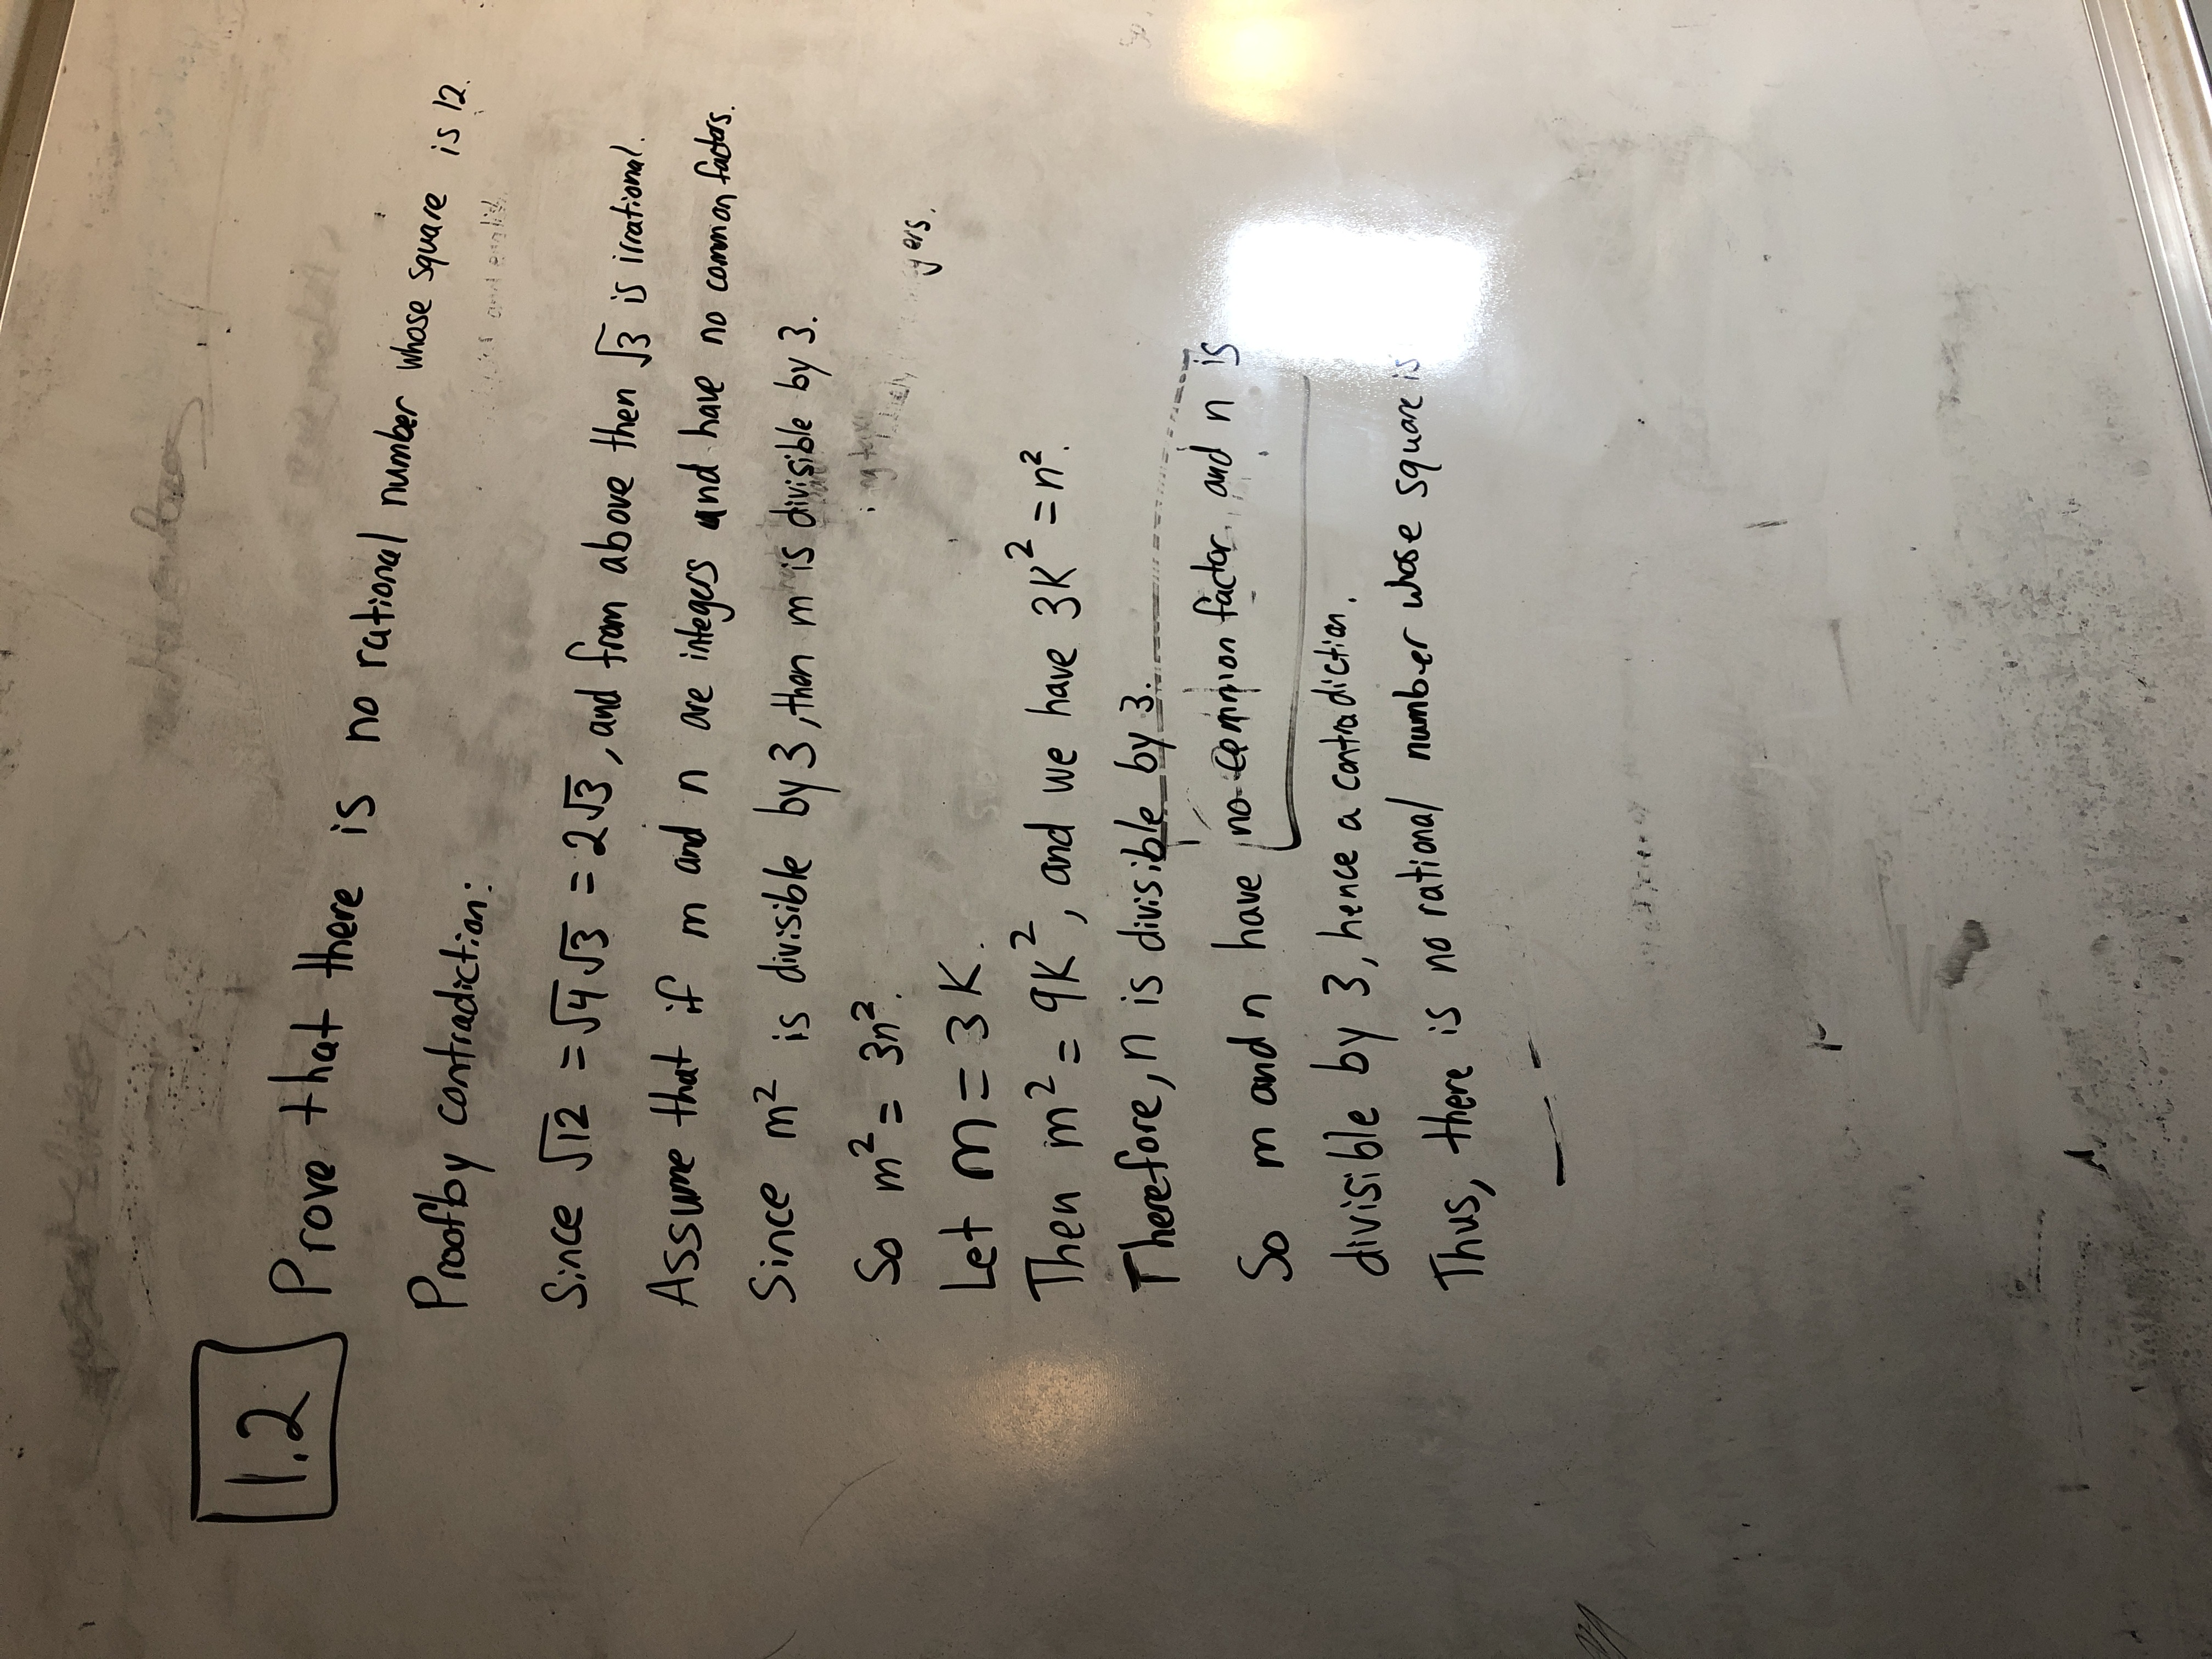
\includegraphics[angle=, origin=c,width=2 in]{Figures/IMG_1077.JPG}
\caption{Placeholder for my proofs} \label{fig:Euler_pic}\end{center}\end{figure} 

\newpage
\section*{5}
(10 points total) Consider the function on $[0,1]$ defined by $f(x)= {x}$ if x is rational 1-x if x is irrational. \\ 
Determine all points at which f(x) is continuous and all points at which it is not continuous.

\begin{figure}[h]\begin{center}\includegraphics[angle=, origin=c,width=2 in]{WhiteboardPictures/Exam 2/IMG_1052.JPG}
\caption{Placeholder for my proofs} \label{fig:Euler_pic}\end{center}\end{figure} 
\newpage

Determine whether f(x) is invertible. Prove all of your conclusions. 

\begin{figure}[h]\begin{center}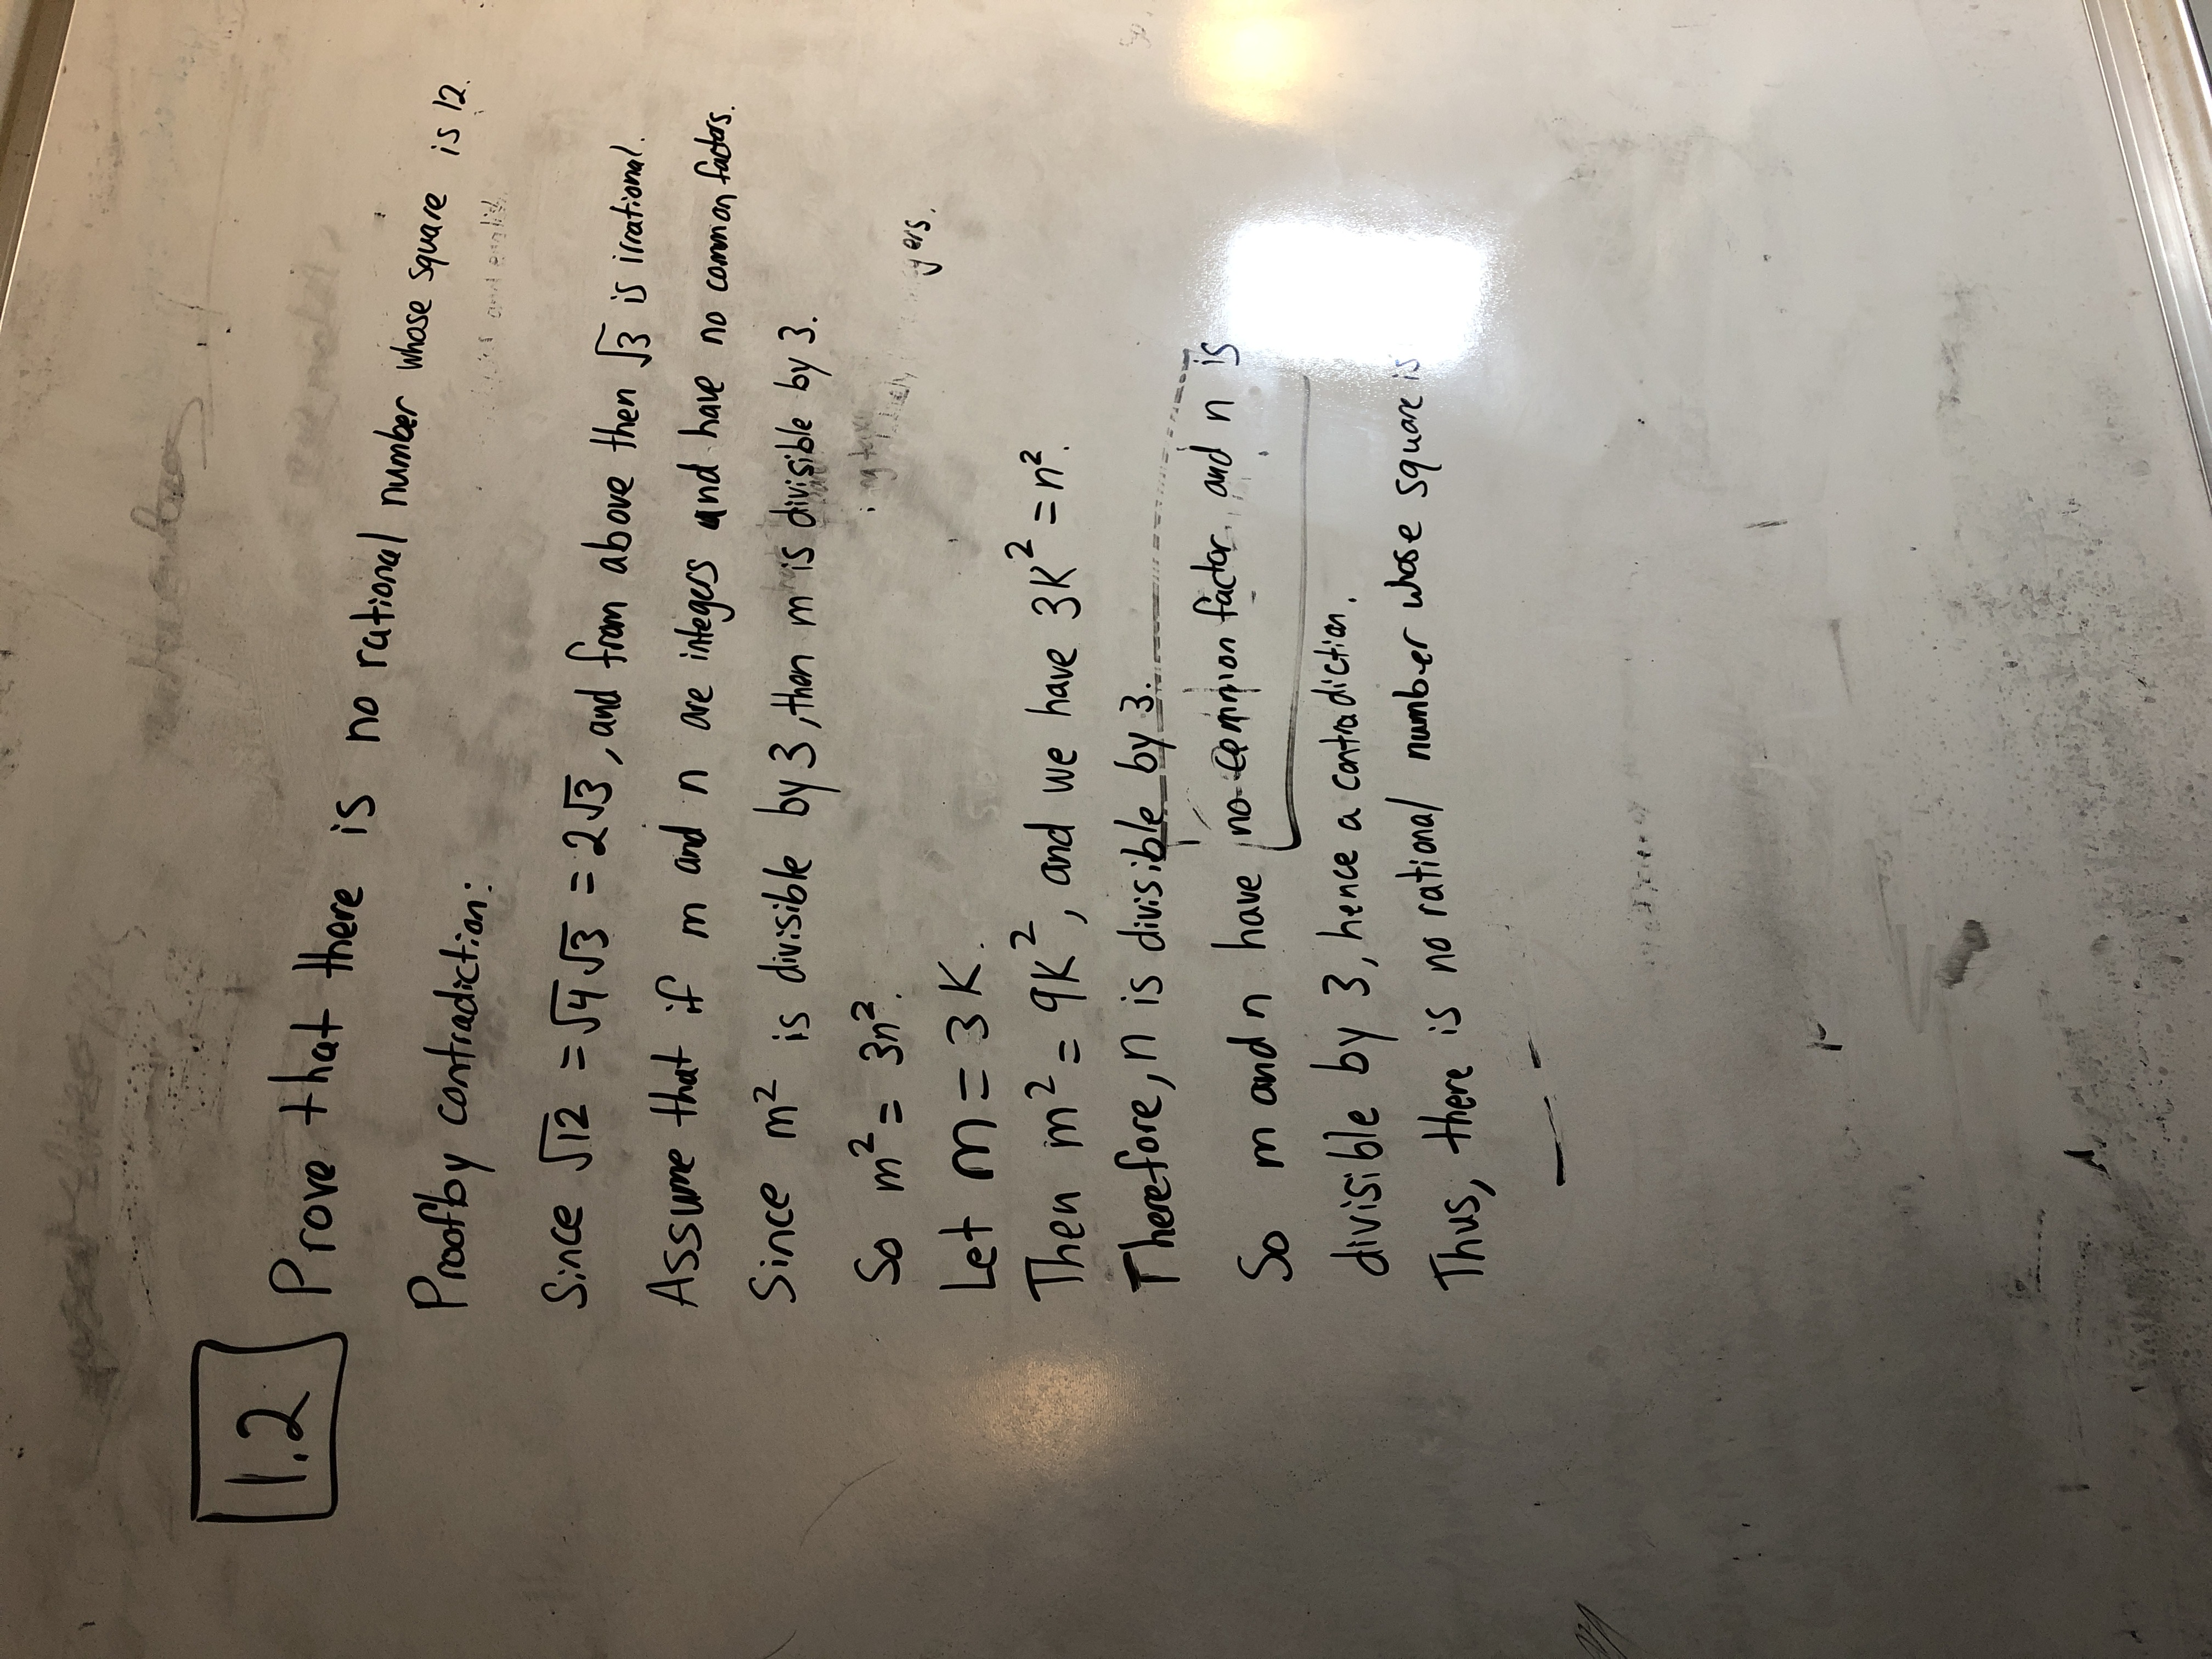
\includegraphics[angle=, origin=c,width=2 in]{Figures/IMG_1077.JPG}
\caption{Placeholder for my proofs} \label{fig:Euler_pic}\end{center}\end{figure} 


\section*{6}
(25 points) 
Let f(x) be continuous on the interval $[a,b].$ Define g(x) so that g(a)= f(a) and, for $x \in (a,b], g(x)$ is the maximum of f(s) for $a \leq s \leq x.$ \\ 
\newpage
Show that g(x) is continuous on the interval $[a,b].$ (5 points) 
\begin{figure}[h]\begin{center}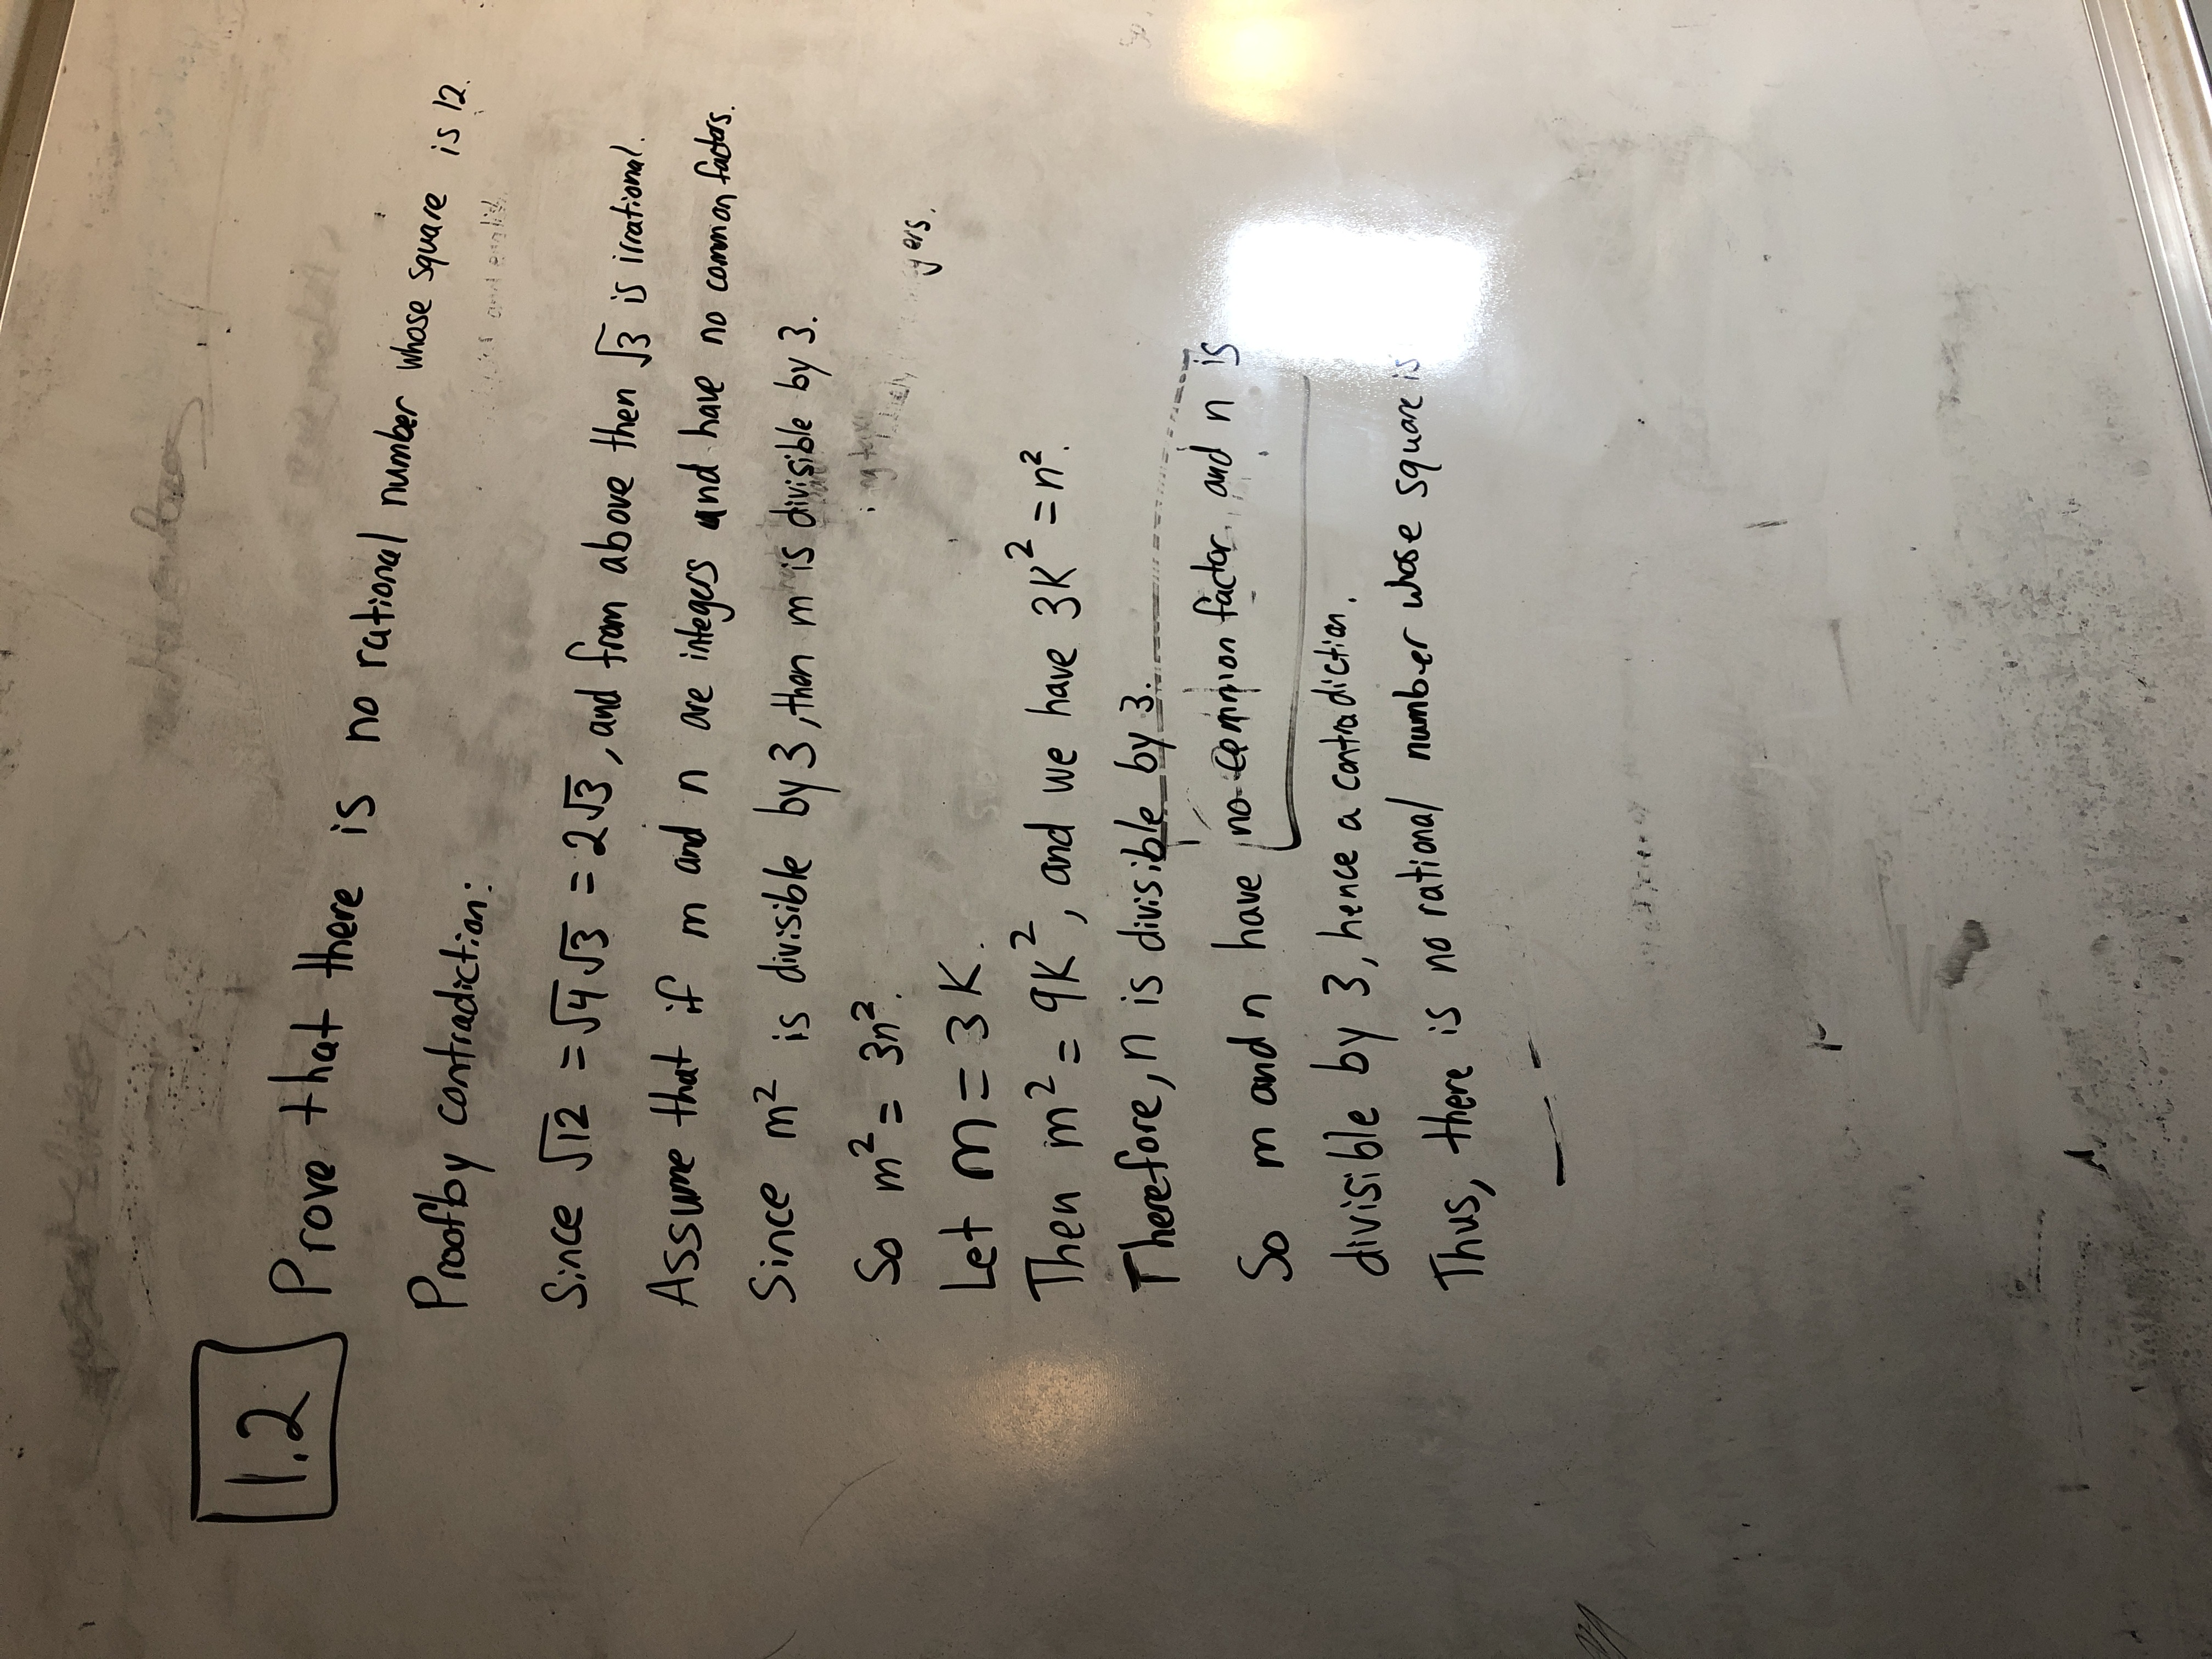
\includegraphics[angle=, origin=c,width=2 in]{Figures/IMG_1077.JPG}
\caption{Placeholder for my proofs} \label{fig:Euler_pic}\end{center}\end{figure} 
Find an example of an interval [a,b] and a function f(x) such that $g(x)=f(x)$ throughout the interval. (3 points). \\
\begin{figure}[h]\begin{center}\includegraphics[angle=, origin=c,width=2 in]{WhiteboardPictures/Exam 2/IMG_1052.JPG}
\caption{Placeholder for my proofs} \label{fig:Euler_pic}\end{center}\end{figure} 
\newpage 
Find an example of an interval $[a,b]$ and a function f(x) such that $g(x) \neq f(x)$ for $x>a.$ (4 points) \\ 

\begin{figure}[h]\begin{center}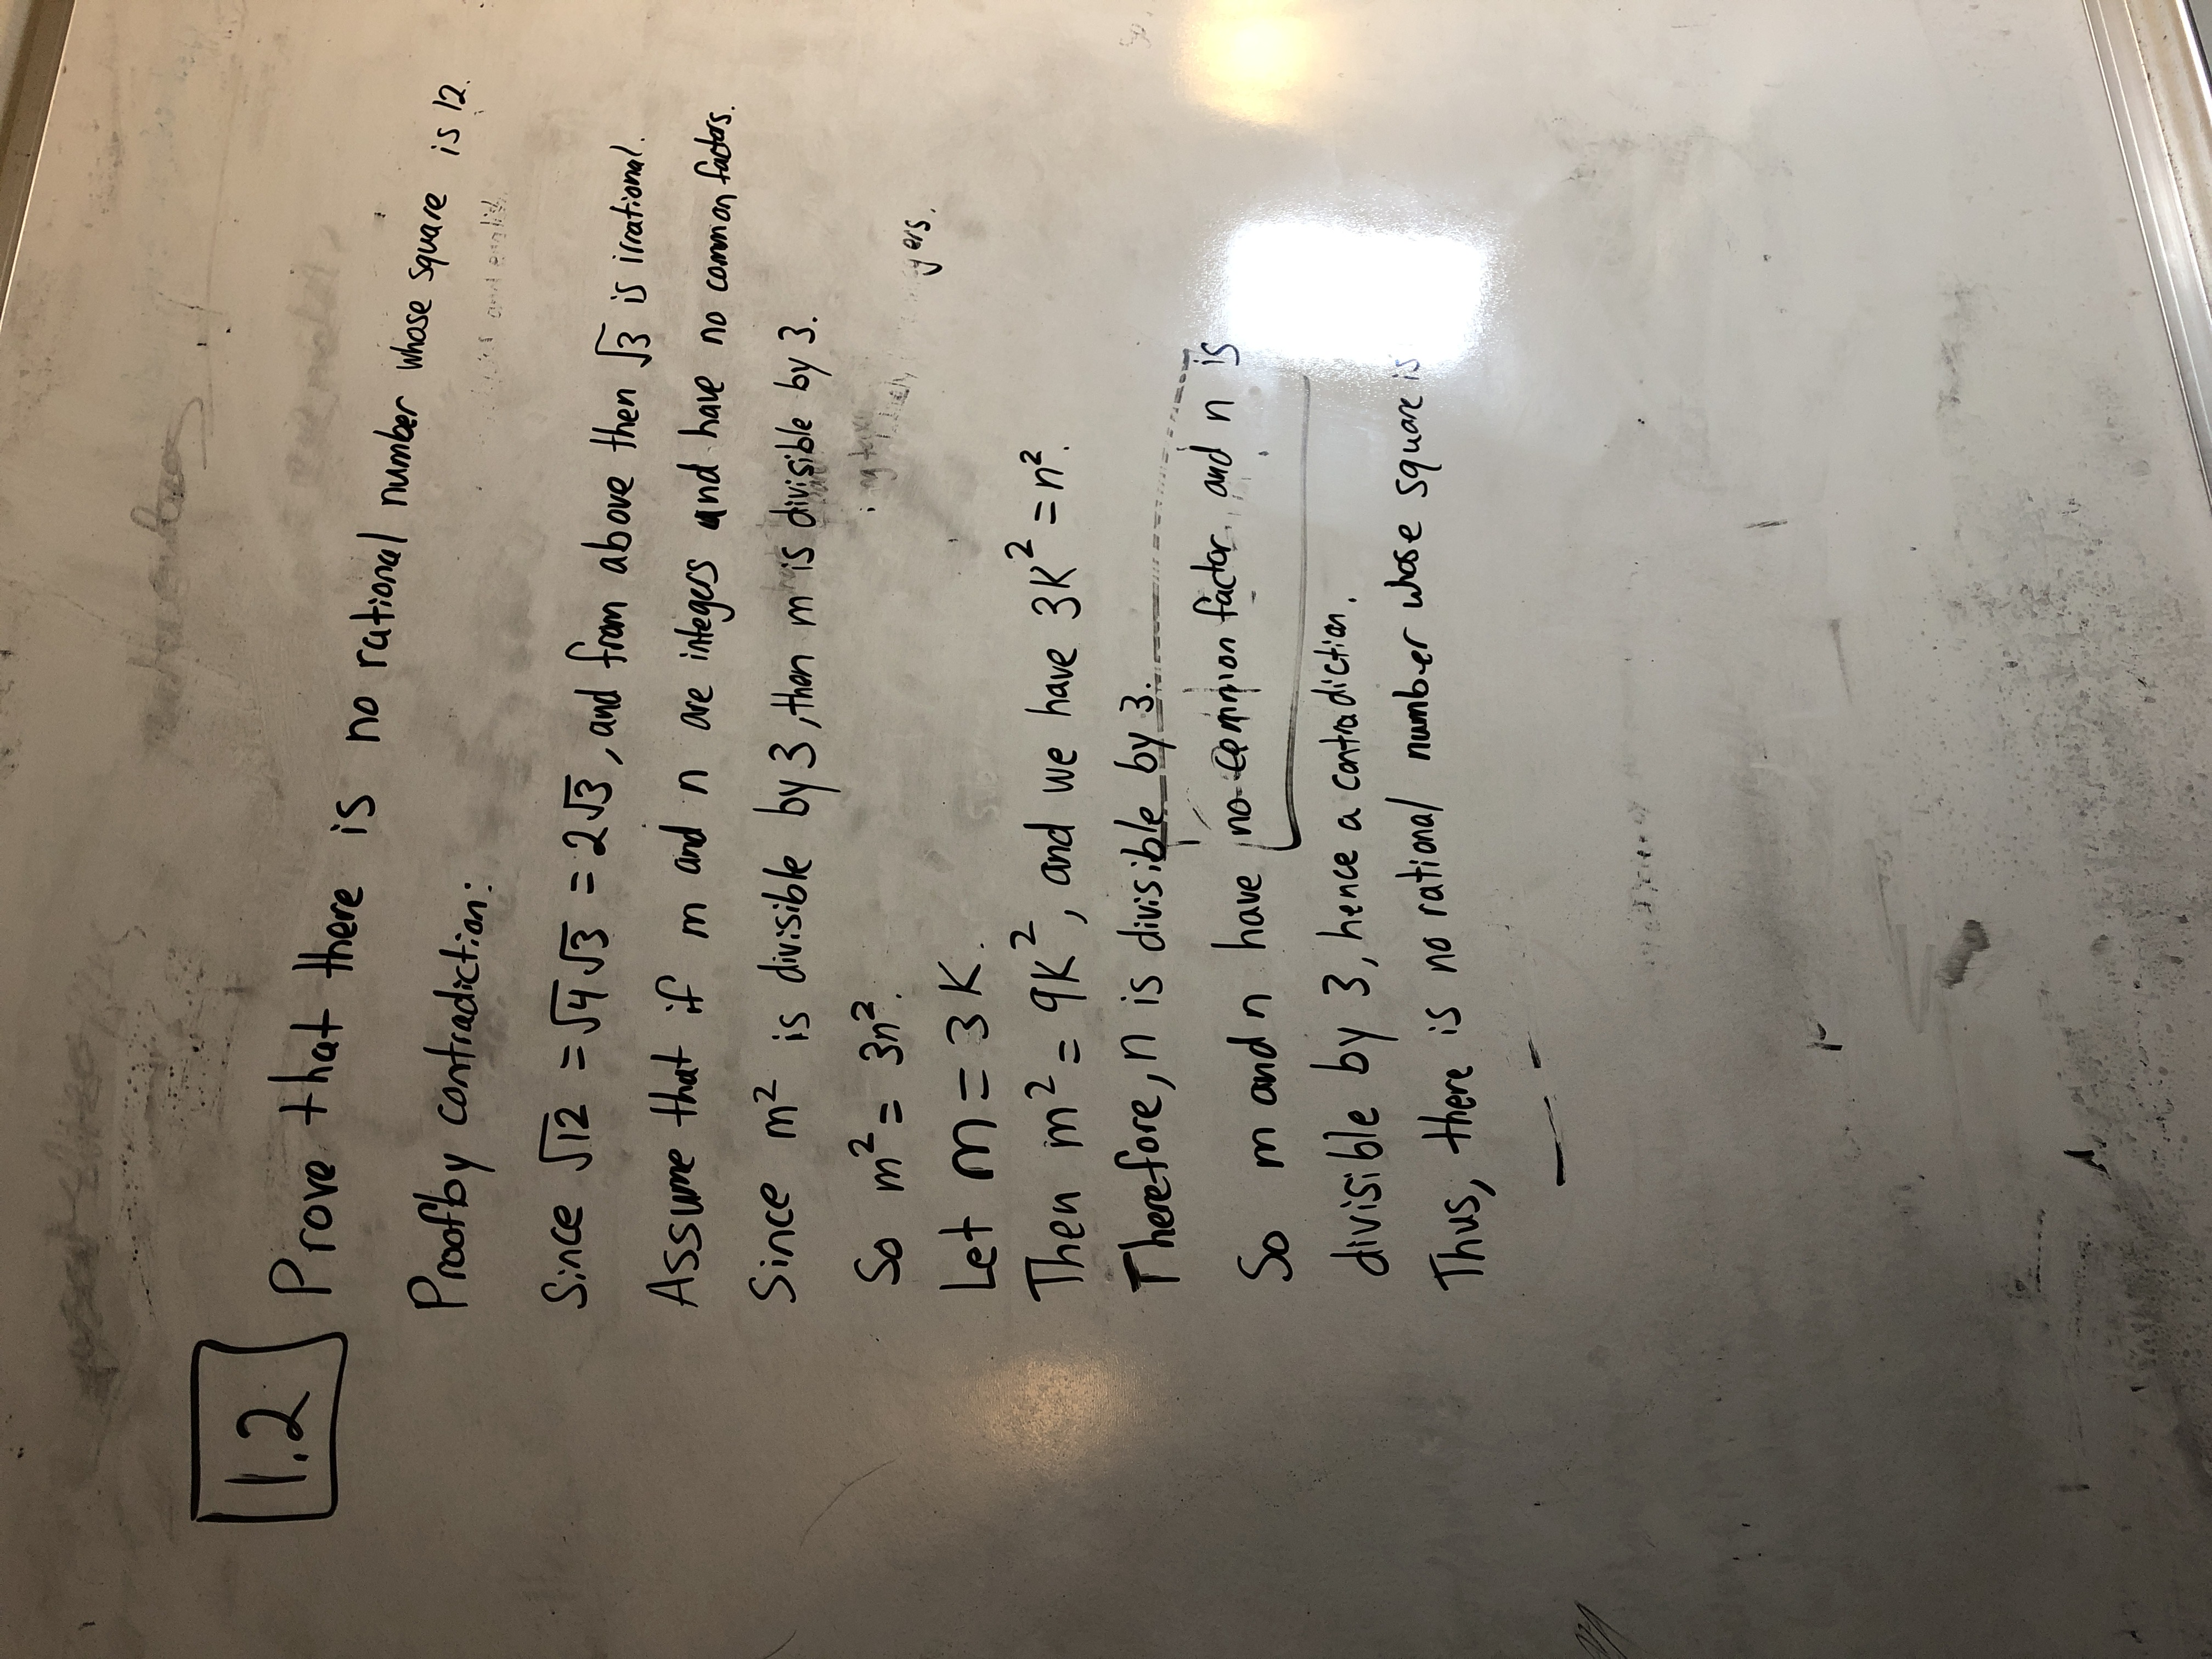
\includegraphics[angle=, origin=c,width=2 in]{Figures/IMG_1077.JPG}
\caption{Placeholder for my proofs} \label{fig:Euler_pic}\end{center}\end{figure} 


Find an example of an interval $[a,b]$ and a function f(x) such that $g(x)=f(x)$ on an open sub-interval whose left endpoint is a, such that $g(x)=f(x)$ on an open sub-interval whose right endpoint is b, and such that $g(x) =\neq f(x)$ on some open sub-interval. Note that you are to find an example of one function with all three of these properties. (4 points) \\ 
\begin{figure}[h]\begin{center}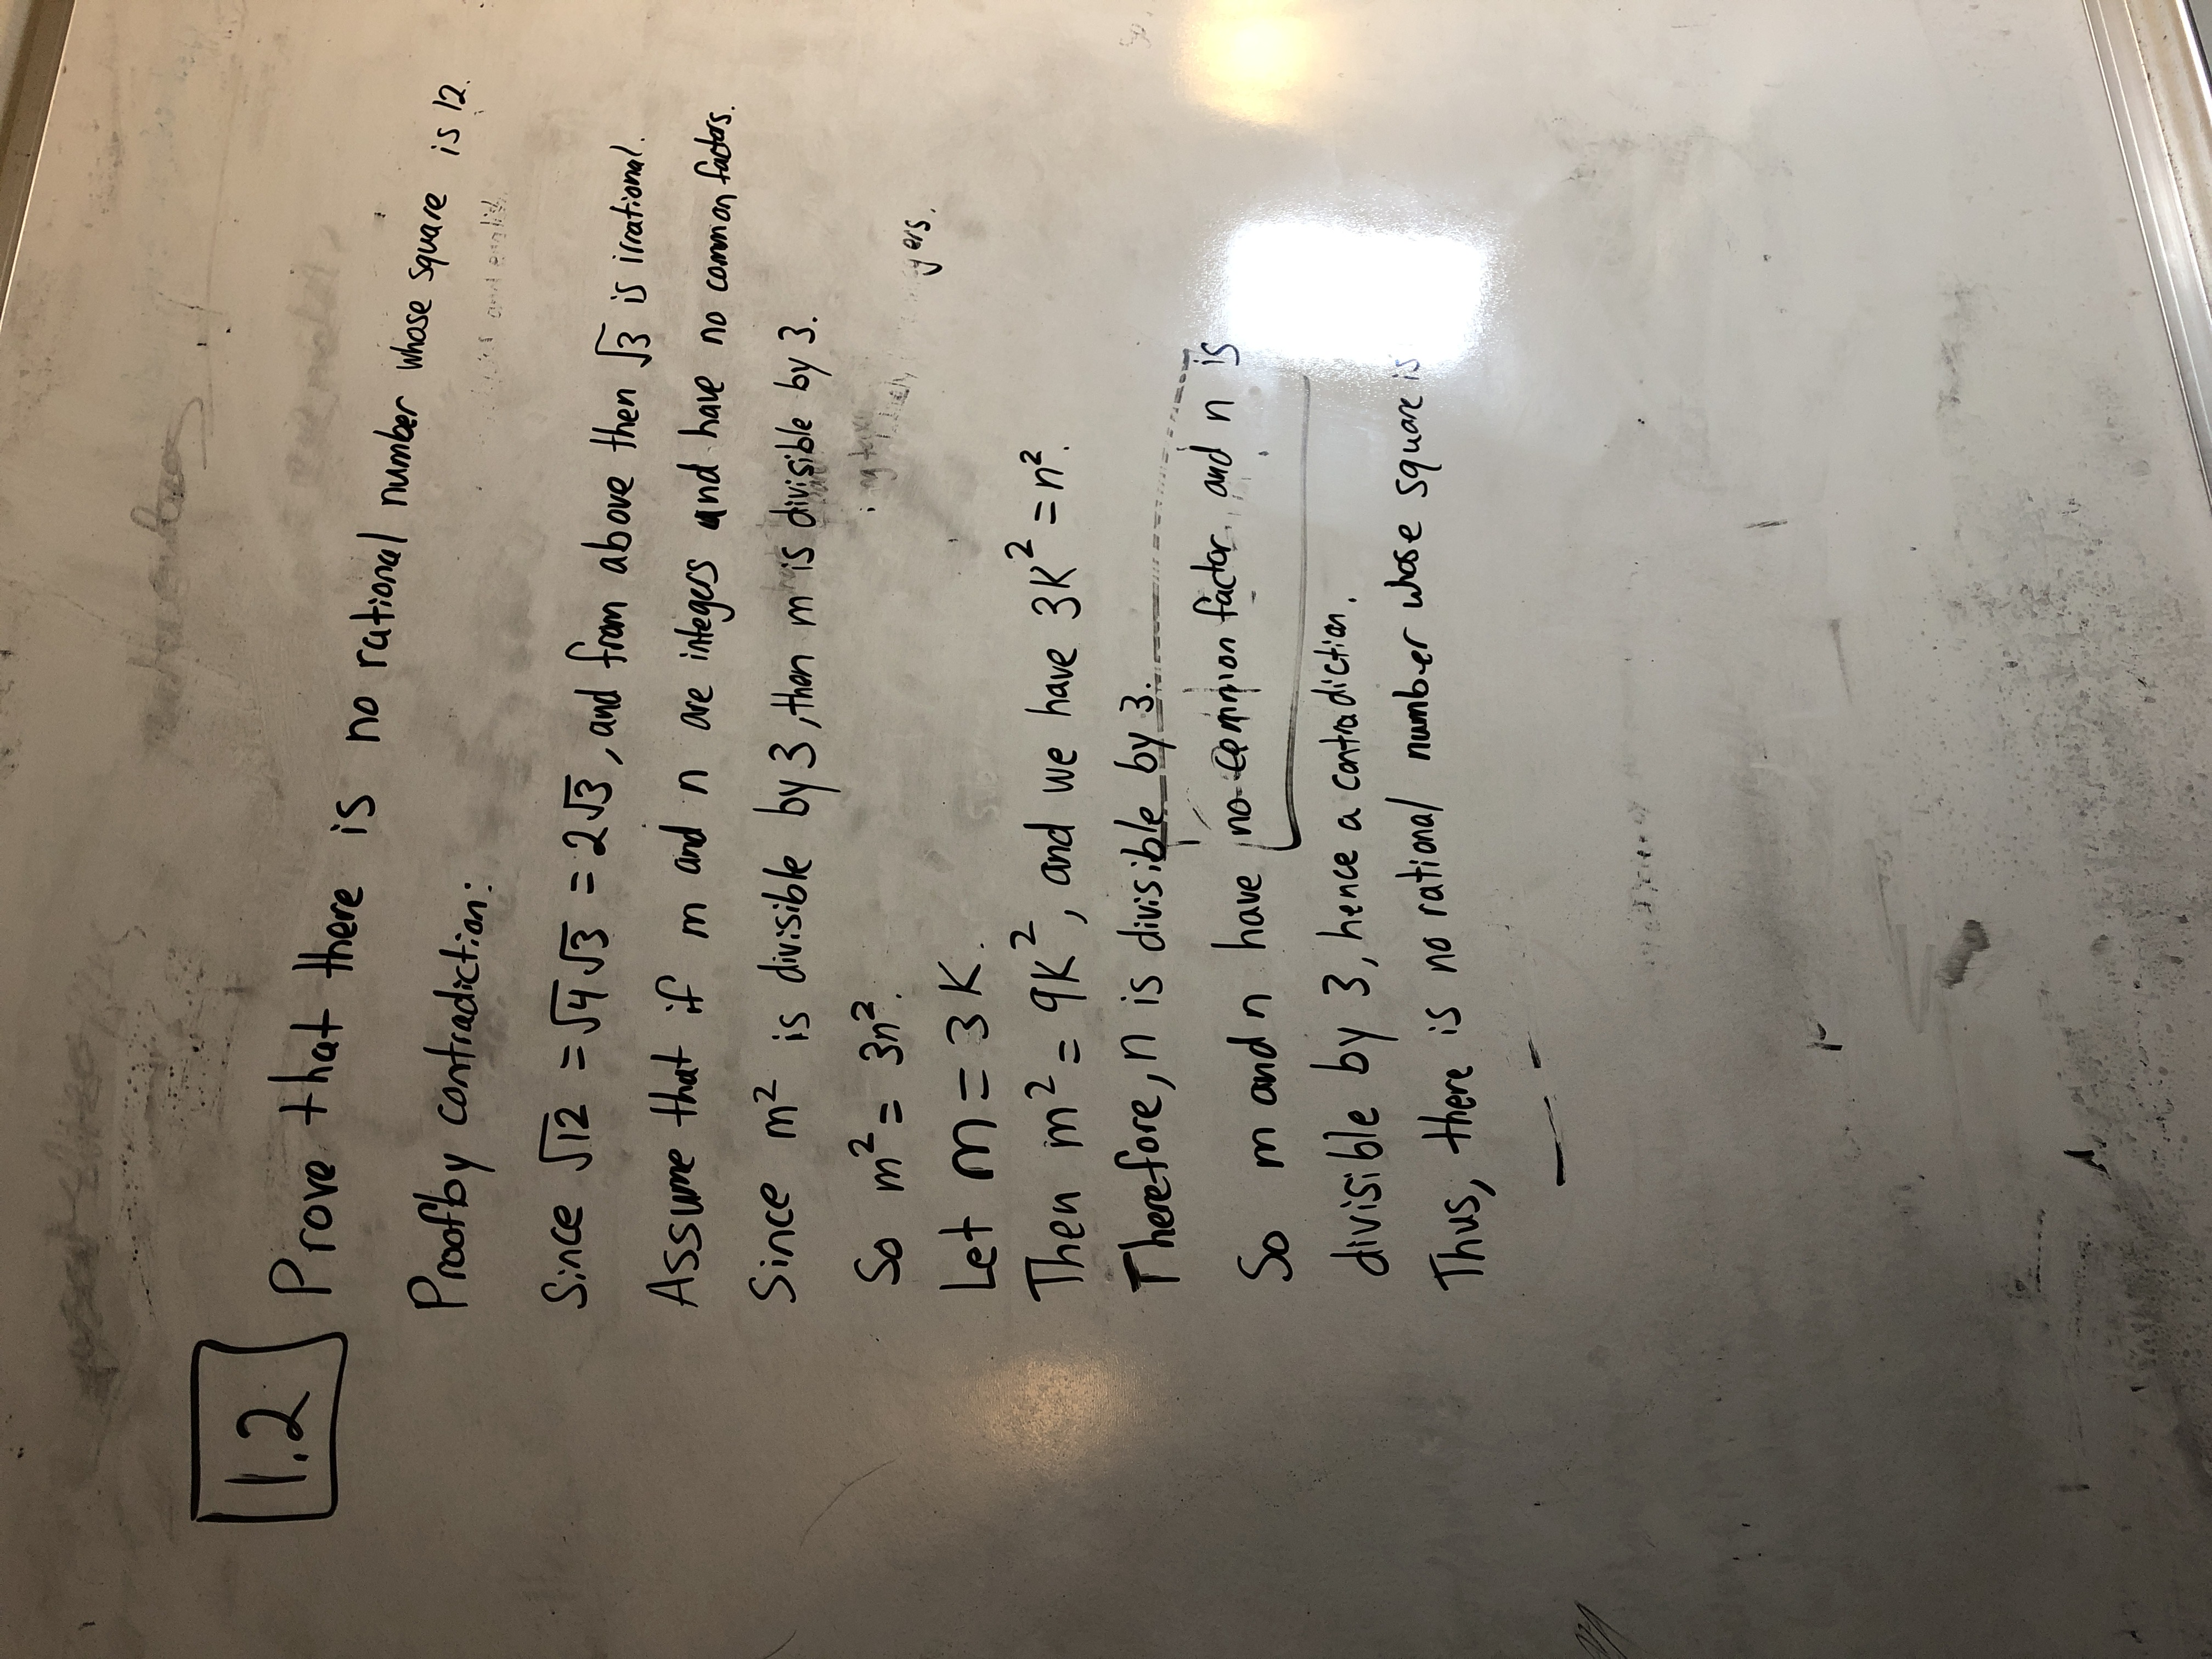
\includegraphics[angle=, origin=c,width=2 in]{Figures/IMG_1077.JPG}
\caption{Placeholder for my proofs} \label{fig:Euler_pic}\end{center}\end{figure} 
\\

\newpage
If f(x) is differentiable, need $g(x)$ be differentiable? Prove your claim. (5 points). \\ 

\begin{figure}[h]\begin{center}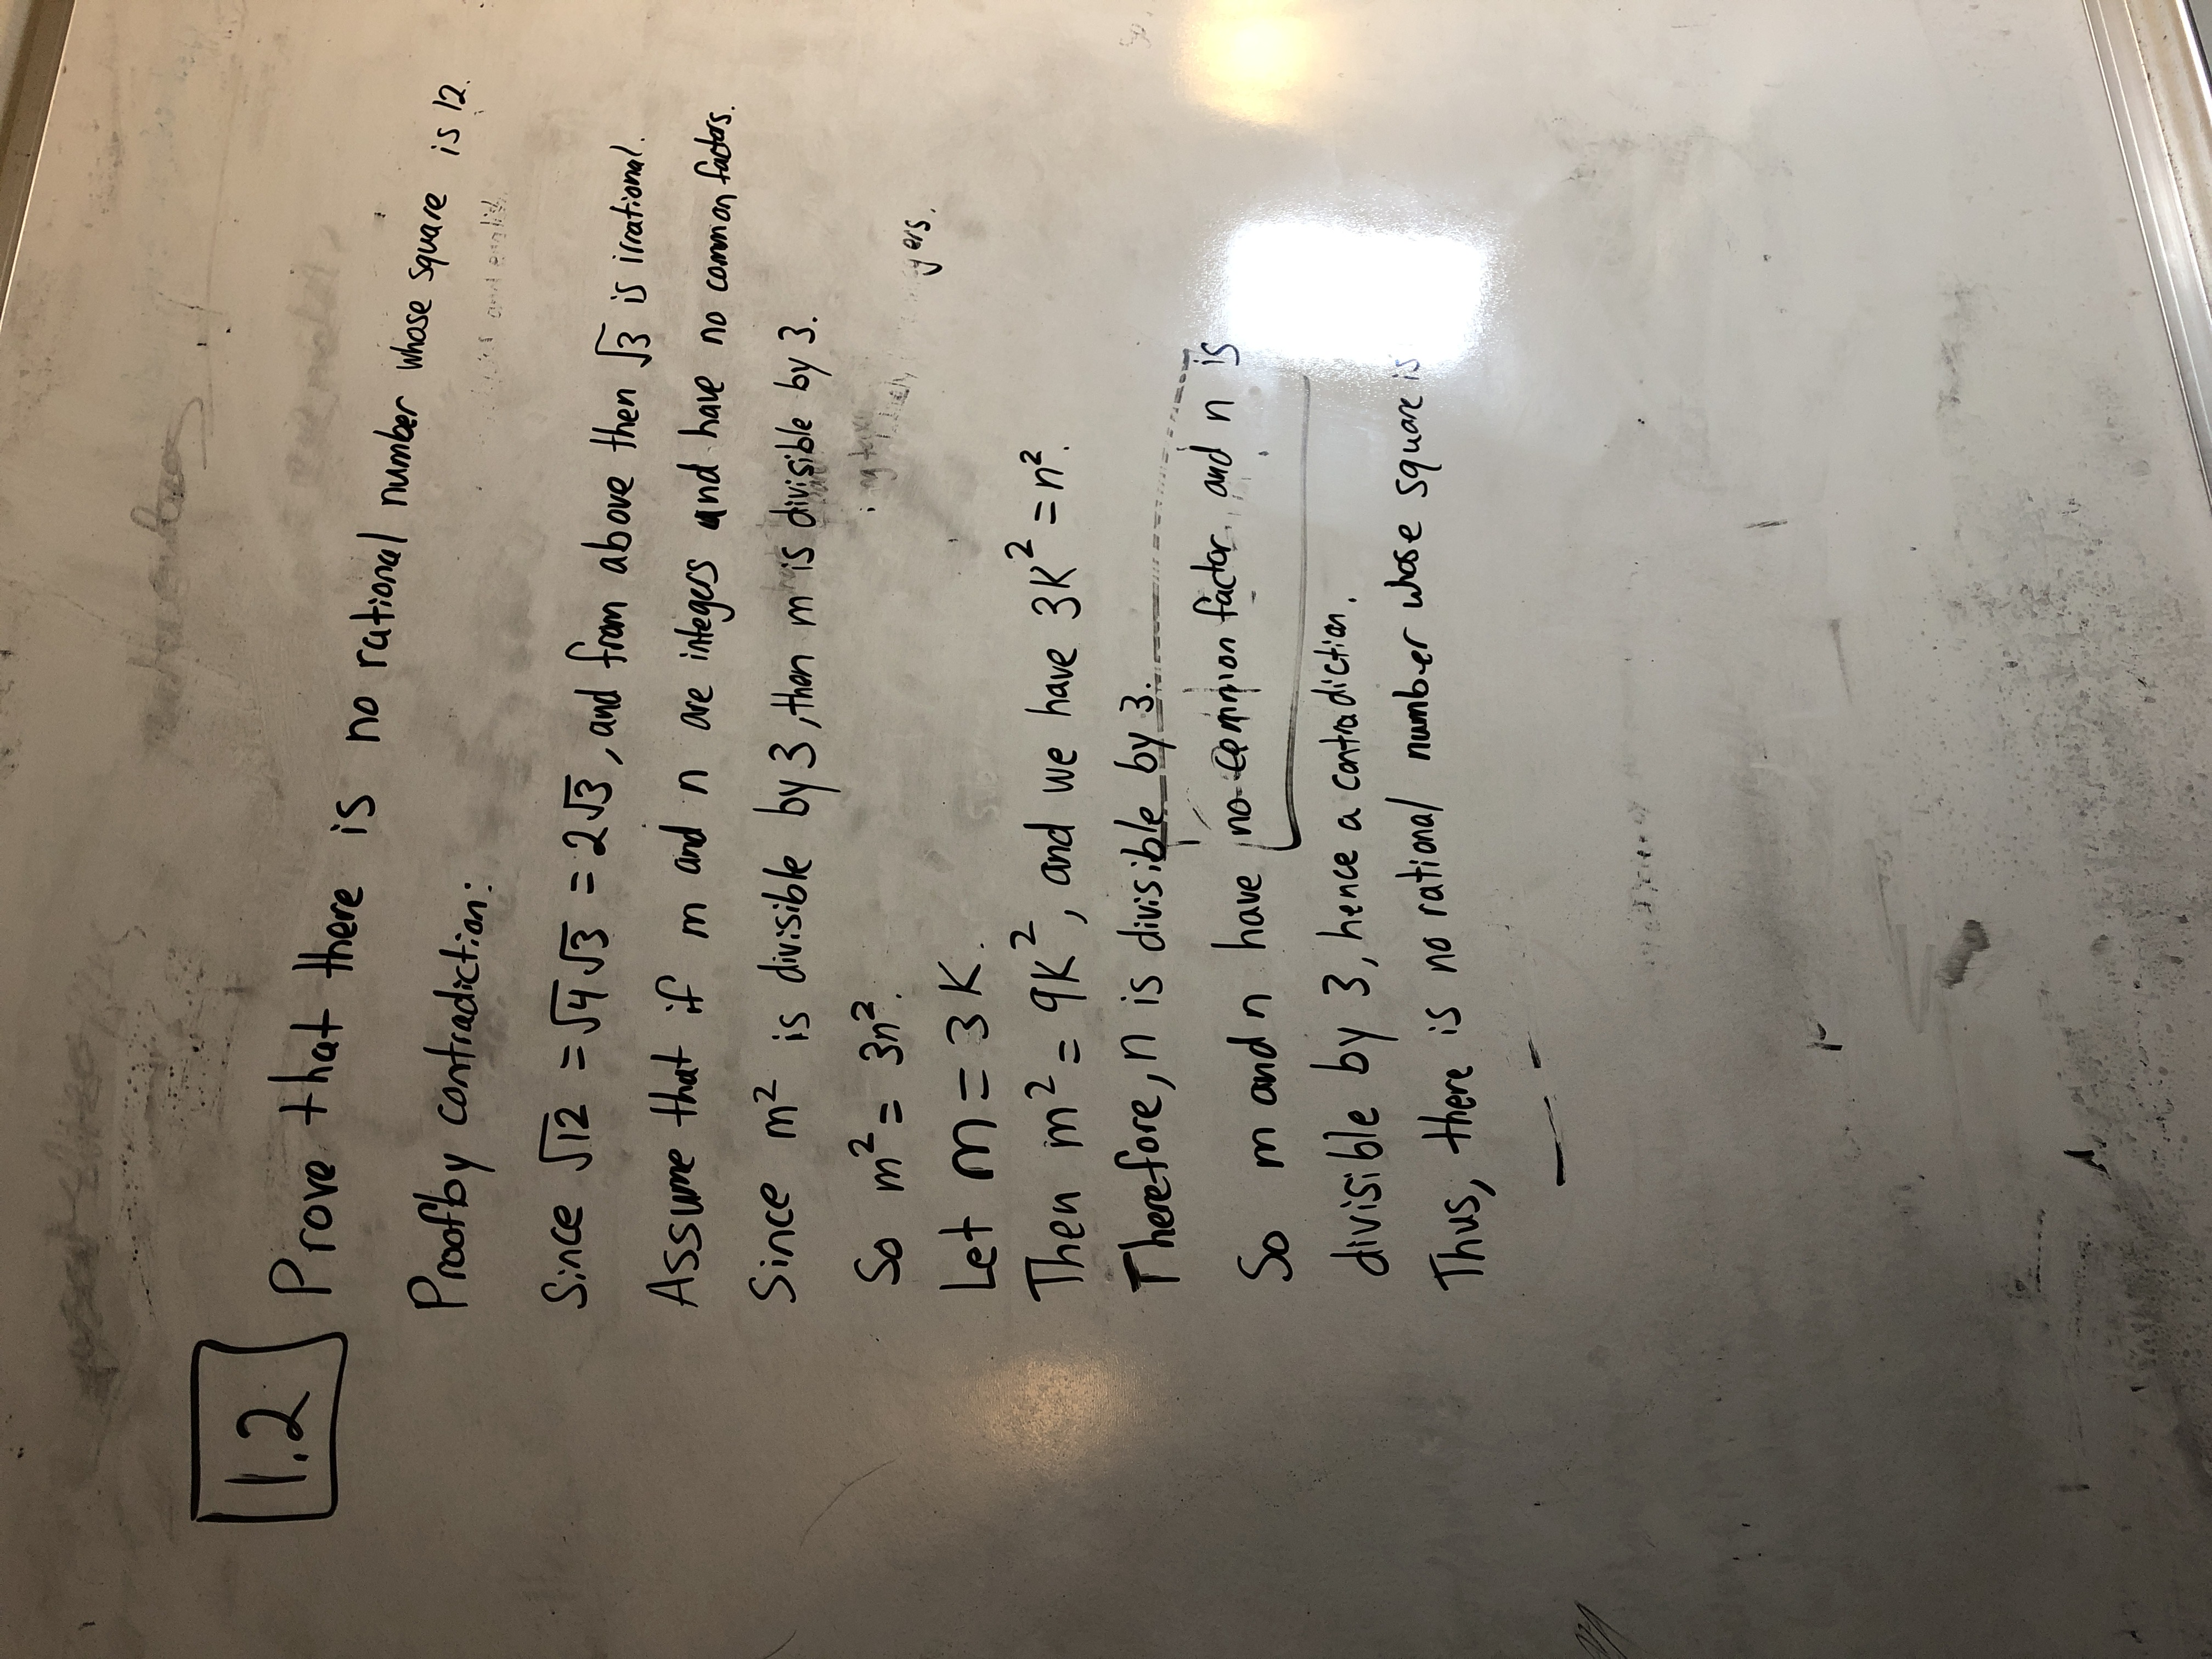
\includegraphics[angle=, origin=c,width=2 in]{Figures/IMG_1077.JPG}
\caption{Placeholder for my proofs} \label{fig:Euler_pic}\end{center}\end{figure} 
\\
\newpage
If f(x) is differentiable, it is possible for g(x) to be differentiable? Prove your claim. (4 points).


\begin{figure}[h]\begin{center}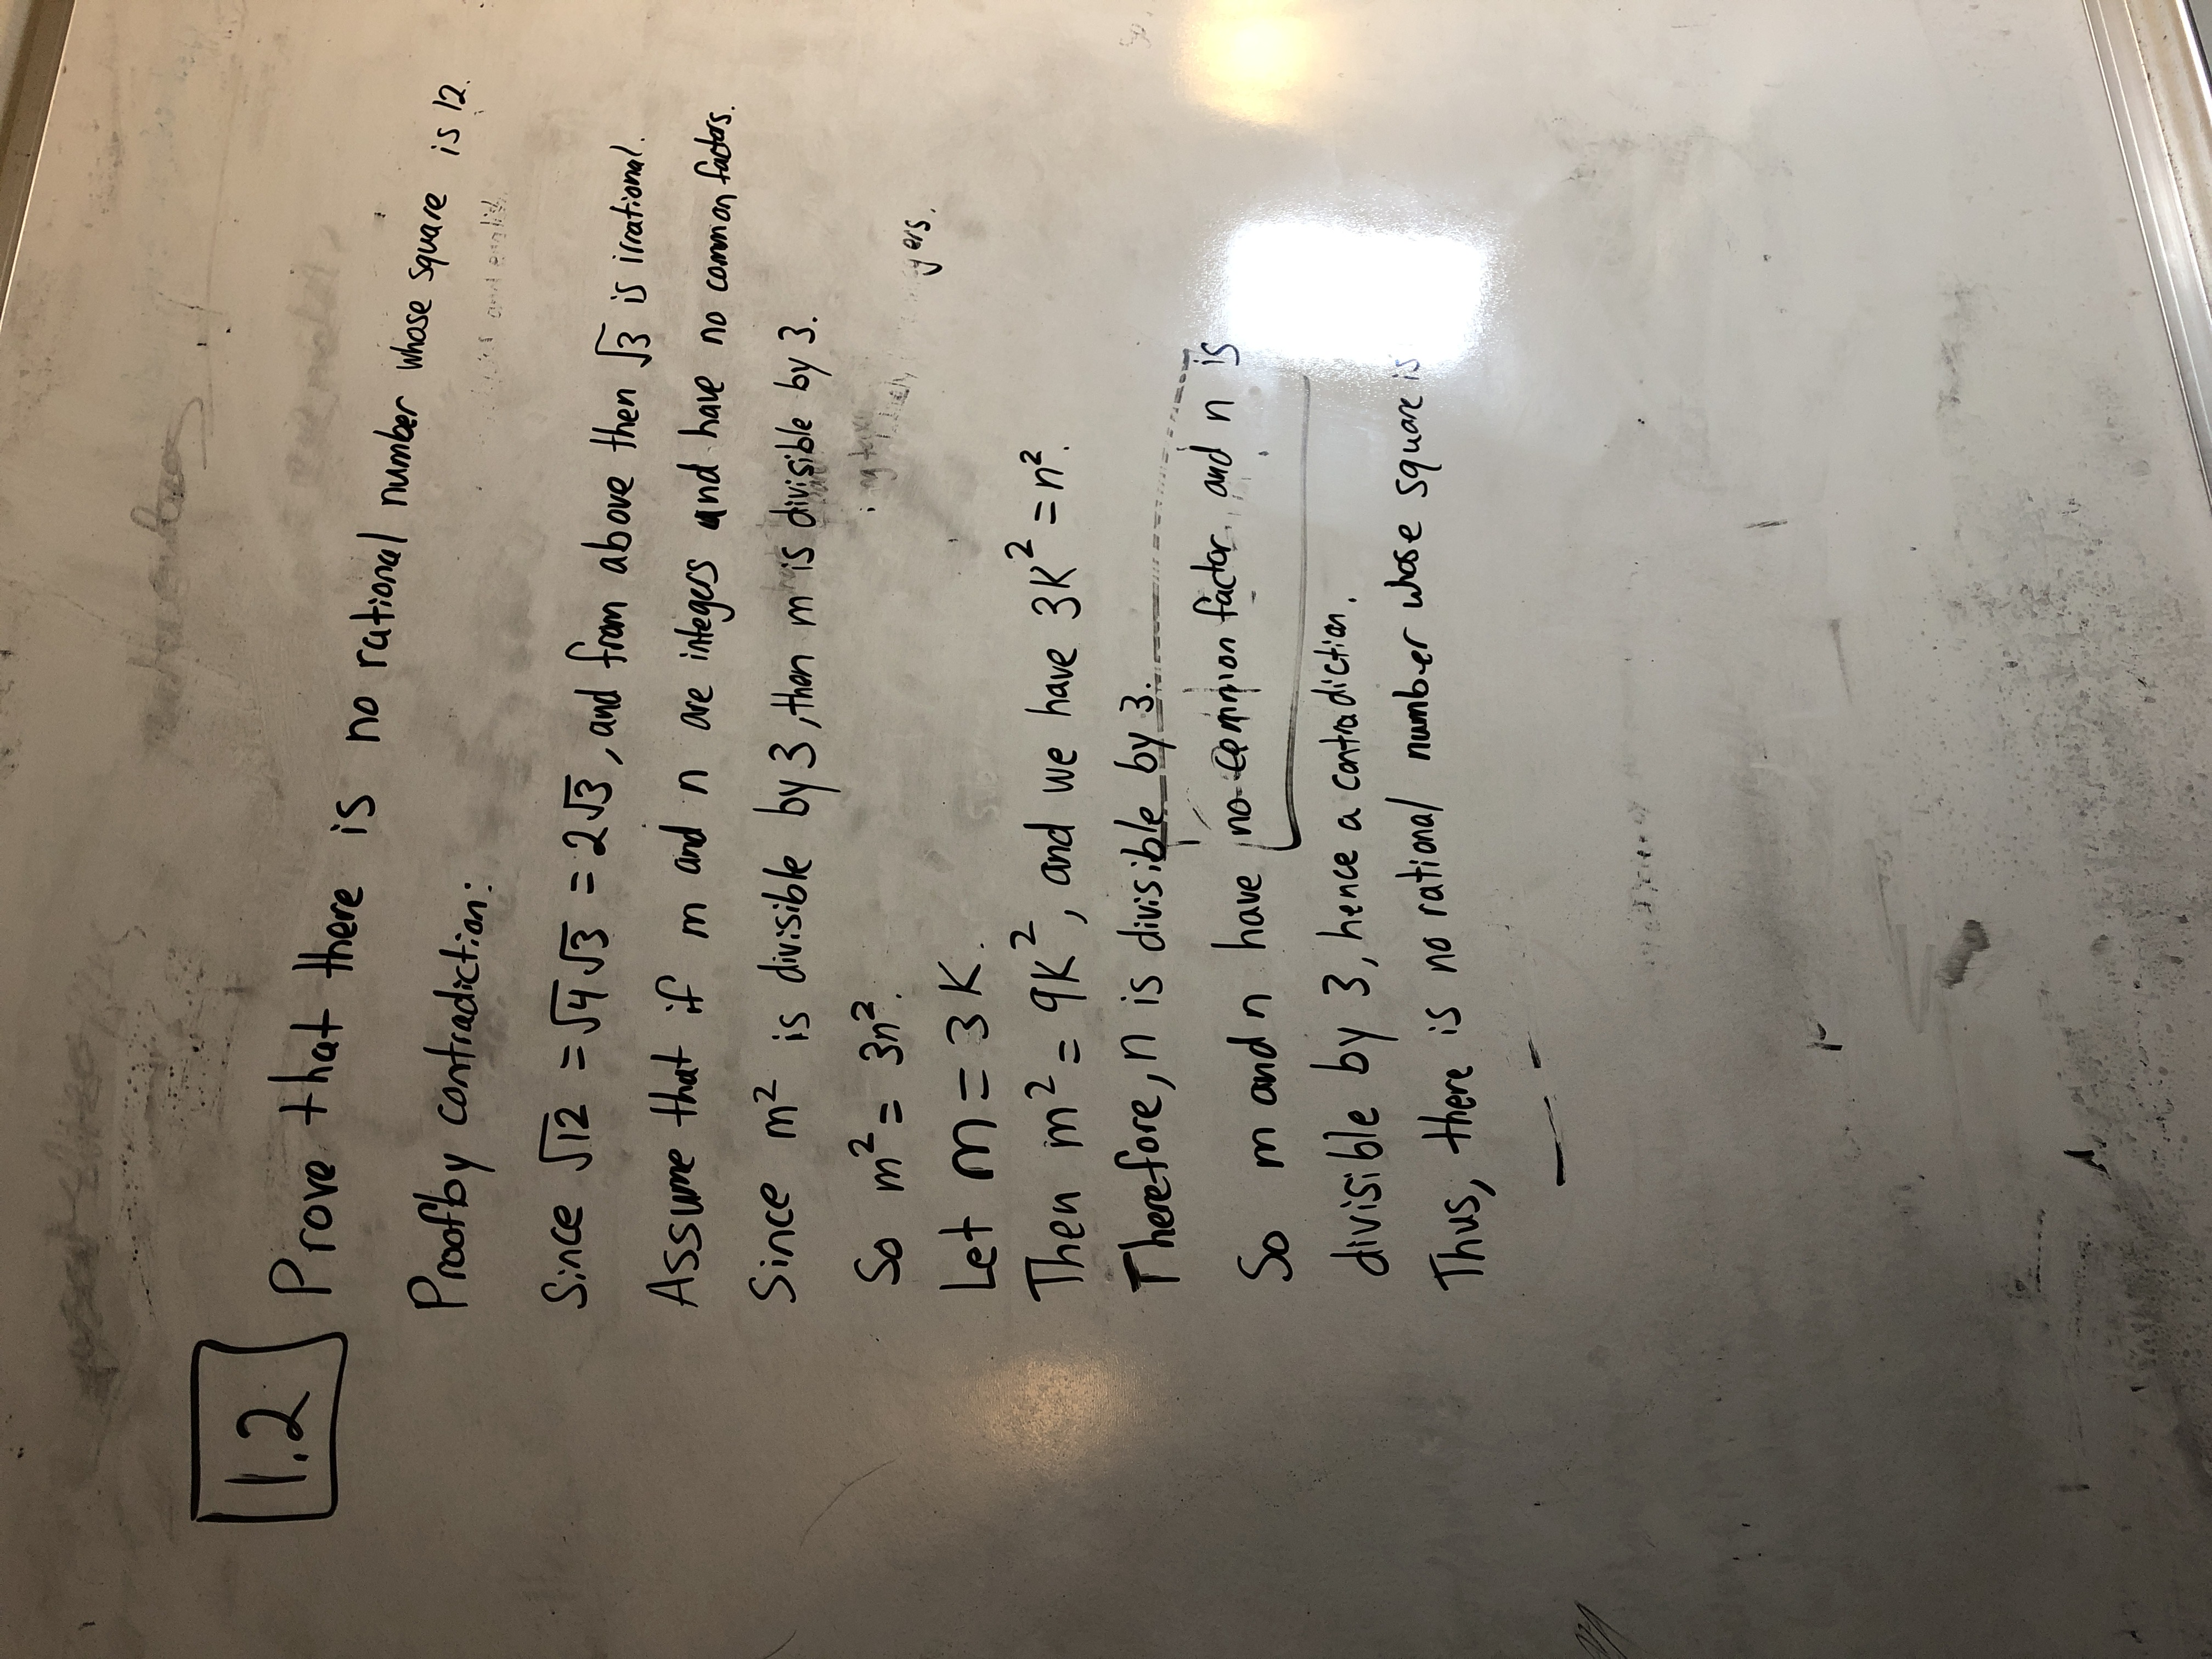
\includegraphics[angle=, origin=c,width=2 in]{Figures/IMG_1077.JPG}
\caption{Placeholder for my proofs} \label{fig:Euler_pic}\end{center}\end{figure} 
\\
\newpage

\section*{7}
(25 points) A function f(x) defined on an interval of $R^1$ is said to be absolutely continuous on that interval if for every $ \epsilon>0 $ there is a $\delta>0$ such that for every collection of disjoint intervals $x_j,y_j) j=1,...,N,$ if $\sum_{j=1}^N y_j -x_j <\delta$ then $\sum_{j=1}^N|f(y_j)-f(x_j)|<\epsilon.$ \\ 
A function f(x) defined on an interval of $R^1$ is said to be Lipschitz on that interval if there is a constant L such that $|f(y)-f(x)| \leq L |y-x|$ for every pair of values x and y in the interval. \\ 






(a) Prove that on a fixed interval every Lipschitz function is absolutely continuous, but that not every absolutely continuous function is Lipschitz.  (5 points) 

\begin{figure}[h]\begin{center}\includegraphics[angle=, origin=c,width=2 in]{WhiteboardPictures/Exam 2/IMG_1052.JPG}
\caption{Placeholder for my proofs} \label{fig:Euler_pic}\end{center}\end{figure} 
\\ 
Let $e>0$ and $\delta= \frac{\epsilon}{M}.$ Then for any collection ${[x_i,y_i}$ of intervals with $\sum |x_i -y_i|<\delta.$ \\ 
Now $\sum |f(x_i)-f(y_i)|<M \sum|x_i-y_i|<e. $ \\
Therefore f is Lipschitz continuous. \\ 
Therefore $\sum|f(x_i)-f(y_i)|<e.$ \\ 

Counter example \\ 
Take $f(x)= \sqrt{x}$ on $[0,k].$ \\ 
$-\sqrt{y} \leq \sqrt{y}.$ \\ 
$\sqrt{x}- \sqrt{y} \leq \sqrt{x} +\sqrt{y}.$ \\ 
$(\sqrt{x}-\sqrt{y})^2 \leq (\sqrt{x}-\sqrt{y})(\sqrt{x}+\sqrt{y})=x-y<\delta.$ \\ 
Therefore $f(x)=f(y)> \sqrt{x}-\sqrt{y}< \sqrt{\delta}= \epsilon.$ \\ 
Choose $\delta=\epsilon^2,$ hence f is absolutely continuous but f(x) =$\frac{1}{2 \sqrt{x}}$ is not bounded. Hence f is not Lipschitz. 

\newpage 
(b) Prove that on a fixed interval every absolutely continuous function is uniformly continuous, but that not every uniformly continuous function is absolutely continuous.  (5 points) 


\begin{figure}[h]\begin{center}\includegraphics[angle=, origin=c,width=2 in]{WhiteboardPictures/Exam 2/IMG_1052.JPG}
\caption{Placeholder for my proofs} \label{fig:Euler_pic}\end{center}\end{figure} 

We have the result that a function satisfying Lipschitz condition is an interval is a uniformly continuous function. \\ 
Hence by (a) an absolutely continuous, uniformly continuous converse is not true. \\ 
Counter example: $f(x)=x^2sin(x)$ on $[0,1]$ \\ 
$f(x)=0$ at x=0. \\


(c)Prove that on a fixed interval every uniformly continuous function is continuous, but that not every continuous function is uniformly continuous.  (5 points) \\ 

\begin{figure}[h]\begin{center}\includegraphics[angle=, origin=c,width=2 in]{WhiteboardPictures/Exam 2/IMG_1052.JPG}
\caption{Placeholder for my proofs} \label{fig:Euler_pic}\end{center}\end{figure} 

Let f: $x \longrightarrow R$ be uniformly continuous then  by definition for any $\epsilon>0$ there exists $\delta>0$ such that $x,y \in X, |x-y|<\delta.$ \\ 
$|f(x)-f(y)<\epsilon.$ \\ 
In particular if we fix $c \in X.$ \\ 
$|x-c|<\delta$ \\ 
$f(x)-f(x)< \epsilon$ for every $c \in X$ f is continuous. \\ 
Converse is not true. \\ 
Counterexample $f(x)=\frac{1}{x}$ in $R^+$ (If we take $x= \frac{1}{n},$ $y=\frac{1}{2}n$ then we can show f is not uniformly continuous.)



Prove that on a fixed interval every differentiable function with bounded derivative is uniformly continuous. (5 points)  

\begin{figure}[h]\begin{center}\includegraphics[angle=, origin=c,width=2 in]{WhiteboardPictures/Exam 2/IMG_1052.JPG}
\caption{Placeholder for my proofs} \label{fig:Euler_pic}\end{center}\end{figure} 

\\ 
Since $f^1$ is bounded then there exists $M>0$ such that $|f(x)|\leq M$ for all x $\in I=[a,b].$ \\ 
Now applying the mean value theorem $f(a)=f(b)=f(\epsilon)(a-b).$ \\ 
In general, $\frac{|f(x)-f(y)|}{|x-y|} \leq M$ \\ 
$|f(x)-f(y)| \leq M|x-y|$ for all x,y $\in I.$ \\ 
So, f is Lipschitz continuous on $I.$ \\ 
F is uniformly continuous. 


\newpage 
Prove that on a fixed interval a differentiable function whose derivative is unbounded may or may not be uniformly continuous. (5 points) 

\begin{figure}[h]\begin{center}\includegraphics[angle=, origin=c,width=2 in]{WhiteboardPictures/Exam 2/IMG_1052.JPG}
\caption{Placeholder for my proofs} \label{fig:Euler_pic}\end{center}\end{figure} 


\section{Chapter 4 Baby Rudin}



\section{Chapter 5 Baby Rudin}


Work work work.




\section{}